%; whizzy chapter
% -initex iniptex -latex platex -format platex -bibtex jbibtex -fmt fmt
% 以上 whizzytex を使用する場合の設定。

%     Tokyo Debian Meeting resources
%     Copyright (C) 2006 Junichi Uekawa

%     This program is free software; you can redistribute it and/or modify
%     it under the terms of the GNU General Public License as published by
%     the Free Software Foundation; either version 2 of the License, or
%     (at your option) any later version.

%     This program is distributed in the hope that it will be useful,
%     but WITHOUT ANY WARRANTY; without even the implied warranty of
%     MERCHANTABILITY or FITNESS FOR A PARTICULAR PURPOSE.  See the
%     GNU General Public License for more details.

%     You should have received a copy of the GNU General Public License
%     along with this program; if not, write to the Free Software
%     Foundation, Inc., 51 Franklin St, Fifth Floor, Boston, MA  02110-1301 USA


%   Pdf作成手順
% dvipdfmx debianmeetingresume200606.dvi
%  preview (shell-command (concat "xpdf " (replace-regexp-in-string "tex$" "pdf"(buffer-file-name)) "&"))
% 画像ファイルを処理するためにはebbを利用してboundingboxを作成。
%(shell-command "cd image200606; ebb *.png")

%%ここからヘッダ開始。

\documentclass[mingoth,a4paper]{jsarticle}
\usepackage[dvipdfmx]{graphicx}
\usepackage{fancybox}
\usepackage{longtable}
\usepackage{ascmac}	% 囲み (screen,itembox)
\usepackage{fancyvrb}   % 囲み Verbatim のために必要
\usepackage[dvipdfmx]{hyperref}
\usepackage{url}
\usepackage[dvipdfmx]{color}

%http://www.naney.org/diki/dk/hyperref.html
%日本語EUC系環境の時
\AtBeginDvi{\special{pdf:tounicode EUC-UCS2}}
%シフトJIS系環境の時
%\AtBeginDvi{\special{pdf:tounicode 90ms-RKSJ-UCS2}}

%% spacing の設定をする。外枠を減らす。
\setlength\headheight{0mm}
\setlength\topmargin{-20mm}
\setlength\headsep{0mm}
\setlength\topskip{3mm}
\setlength\maxdepth{4pt}
\setlength\columnsep{6mm}
\setlength\textheight{252mm}
\setlength\topmargin{-5mm}
\setlength\textwidth{170mm}
\setlength\oddsidemargin{-5mm}
\setlength\evensidemargin{-5mm}

% commandline環境を定義。画面入出力についてはcommandline環境
% で表記する
\newenvironment{commandline}%
{\VerbatimEnvironment
  \begin{Sbox}\begin{minipage}{15cm}\begin{fontsize}{7.3}{7.3} \begin{BVerbatim}}%
{\end{BVerbatim}\end{fontsize}\end{minipage}\end{Sbox}
  \setlength{\fboxsep}{8pt}\fbox{\TheSbox}}


%%% start of santaku
\makeatletter
\newwrite\tf@jqz
\immediate\openout\tf@jqz\jobname.jqz\relax
\makeatother
\newcounter{santakucounter}
\newcommand{\santaku}[5]{%
\addtocounter{santakucounter}{1}

\addtocontents{jqz}{\arabic{santakucounter}. #5\\}
\begin{minipage}{1\hsize}
問題\arabic{santakucounter}. 
#1\\
□ A #2\\
□ B #3\\
□ C #4
\end{minipage}
\hspace{1cm}
\\


}
%%% end of santaku

\newcommand{\emptyspace}{(\underline{\hspace{1cm}})}

\newcommand{\subsubsubsection}[1]{%
\vspace{1zw}{\bf #1}\\}

% sectionをセンタリングする
\makeatletter
  \renewcommand{\section}{\@startsection{section}{1}{\z@}%
    {\Cvs \@plus.5\Cdp \@minus.2\Cdp}% 前アキ
    {.5\Cvs \@plus.3\Cdp}% 後アキ
    {\normalfont\Huge\headfont\raggedright\centering}} % style
\makeatother

% section の代わりの環境
\newcommand{\dancersection}[2]{%
\newpage
東京エリアDebian勉強会 2006
\hrule
\vspace{0.5mm}
\hrule
%\hfill{}
\includegraphics[width=3cm]{image200502/openlogo-nd.eps}\\
\hfill{}
\includegraphics[width=16cm]{image2006-natsu/guruguru-sand-light.png}\\
\vspace{-5cm}
\begin{center}
\section{#1}
\end{center}
\hfill{}\colorbox{white}{#2}\hspace{3cm}\space\\
\vspace{1cm}
\hrule
\vspace{0.5mm}
\hrule
\vspace{1cm}
}

% for dancerj
\newcommand{\fgref}[1]{図\ref{#1}}
\newcommand{\tbref}[1]{表\ref{#1}}

\begin{document}

\begin{titlepage}

% 毎月変更する部分
\title{
あんどきゅめんてっどでびあん}
\date{}
\author{\bf 東京エリアDebian勉強会} 
%\maketitle  % use the graphics instead of the text

\includegraphics[height=252mm]{image2006-natsu/titlepage-summer.eps}

%\thispagestyle{empty}
\end{titlepage}

\newpage
\setcounter{tocdepth}{1}
\tableofcontents
\vspace{6cm}

\large
\begin{itembox}{\bf『あんどきゅめんてっど でびあん』について}
本書は、東京周辺で毎月行なわれている『東京エリア Debian 勉強会』で
使用された資料・小ネタ・必殺技などを一冊にまとめたものです。
収録範囲は勉強会第11回から第17回まで。
内容は無保証、つっこみなどがあれば勉強会にて。
\end{itembox}
\normalfont


\dancersection{Debian Policy 入門 第1回}{岩松 信洋}

\subsection{Debianポリシーとは}
    Debian GNU/Linuxのポリシーです。
    Debian GNU/Linuxとして守るべき方針についてまとめられたものです。
    Debianパッケージの内部構成やオペレーティングシステムとして必要
    な設計部について示されており、ドキュメント化されています。

    これらのドキュメントには debian-policy マニュアルと他の部分に
    ついて補足するサブポリシーマニュアル があります。
    現在のdebian-policy マニュアルバージョンは 3.6.2.2 です。
    毎日議論され、修正が加えられています。


\subsection{debian-policyマニュアルの構成}
    deian-policyマニュアルの構成はどうなっているのか。

    主にDebianパッケージの内容になっています。
    以前はdebian-policyマニュアルとDebian パッケージングマニュアルに
    分かれていたのですが、統合されました (3.2.1.1で統合) 。

    以下にdebian-policyの内容をリストにしてみました。

    \subsubsection{Debianアーカイブ}
\begin{itemize}
        \item Debian Free Software Guidelines (DFSG)とはなにか
        \item main / contrib / non-free セクションの説明および
          各セクションに収録されるパッケージの条件について
        \item Copyrightの問題について
        \item サブセクションについて
        \item パッケージに対するプライオリティについて
\end{itemize}
    \subsubsection{バイナリパッケージについて}

\begin{itemize}
        \item パッケージ名について
        \item パッケージのバージョンについて
            日付に基づいたバージョン番号の付け方

        \item メンテナーのパッケージについて
        \item パッケージの説明について
            パッケージの簡単な説明について
            パッケージの詳細な説明について

        \item パッケージの依存について
        \item バーチャルパッケージ
        \item ベースシステムについて
        \item エッセンシャルなパッケージについて
        \item メンテナースクリプト
\end{itemize}

    \subsubsection{ソースパッケージについて}
\begin{itemize}
        \item 規格への対応
        \item パッケージ関係
        \item 上流パッケージソースの変更について
        \item Debian changelog(debian/changelog)
            代替のchangelog形式
        \item Makefile内でのエラーのトラップについて
        \item タイムスタンプスタンプ
        \item ソースパッケージの中の物における制限
        \item メインビルドスクリプト: (debian/rules)
        \item Variable substitutions: (debian/substvars)
        \item 生成されたパッケージリスト: (debian/file)
\end{itemize}

    \subsubsection{コントロールファイルについて}
\begin{itemize}
        \item コントロールファイルの構文について
        \item ソースパッケージ制御ファイル(debian/control)
        \item バイナリパッケージ制御ファイル(debian/control)
        \item Debianソース制御ファイル--.dsc
        \item Debian Change ファイル--.changes
        \item コントロールファイルのフィールドリスト
        \item ユーザによって定義されたフィールド
\end{itemize}

    \subsubsection{パッケージメンテナンススクリプトとパッケージがインストールされる手順について}
\begin{itemize}
        \item パッケージメンテナスクリプトの序論
        \item メンテナスクリプトの再入結果の同一性
        \item メンテナンススクリプトからのターミナルの制御
        \item メンテナンススクリプトの呼ばれ方の詳細
        \item インストールおよびアップグレードのアンパックフェーズの詳細
        \item 詳細な構成
        \item パッケージの削除とパッケージ設定の完全削除の詳細
\end{itemize}

    \subsubsection{パッケージ同士の関係について}
\begin{itemize}
        \item パッケージ関係フィールドの構文
        \item バイナリの依存について
            (Depends, Recommends, Suggests, Enhances, Pre-Dependsの説明)
        \item バイナリパッケージのコンフリクト( Conflicts )
        \item バーチャルパッケージ( Provides)
        \item ファイルを上書きし、パッケージを置き換える( Replaces )
            他のパッケージの中のファイルを上書きする
            パッケージの削除を強制して、全体のパッケージを置き換える
\end{itemize}

    \subsubsection{共有ライブラリについて}
\begin{itemize}
        \item ldconfig
        \item ランタイムサポートプログラム
        \item スタティックライブラリ
        \item 開発ファイル
        \item 同じライブラリのパッケージとのの依存関係
        \item ライブラリと他のパッケージとの依存 ( shlibsシステム )
            システム上の現在のshlibsファイル
            dpkg-shlibdepsとshlibsファイルの使い方について
            shlibs File フォーマット
            shlibsファイルの提供する
            debian/shlibs.local file を書く
\end{itemize}
    \subsubsection{オペレーティングシステムについて}
\begin{itemize}
        \item ファイルシステム階層構造 ( FHS )
        \item ユーザとグループ
        \item システムランレベルとinit.dスクリプト
        \item init.dスクリプトからのコンソールメッセージ
        \item Cron ジョブ
        \item メニュー
        \item Multimedia handler( MIME )
        \item キーボード構成
        \item 環境変数
        \item doc-baseパッケージを使ったドキュメントの登録方法
\end{itemize}
    \subsubsection{各種ファイルについて}
\begin{itemize}
        \item バイナリファイル
        \item ライブラリファイル
        \item 共有ライブラリ
        \item スクリプト
        \item シンボリックリンク
        \item デバイスファイル
        \item 設定ファイル
        \item ログファイル
        \item パーミッションと所有者
\end{itemize}

    \subsubsection{アプリケーションの変更について}
\begin{itemize}
        \item アーキテクチャ指定のための文字列
        \item デーモン
        \item 仮想tty の使用、wtmp,utmp,lastlog等の更新について
        \item エディタとページャについて
        \item Webサーバーとアプリケーション
        \item メール配送、配信、ユーザーエージェント
        \item ニュースシステムの設定
        \item X Window System 用のプログラム
        \item Emacs Lisp プログラム
        \item ゲーム
\end{itemize}
    \subsubsection{ドキュメントについて}
\begin{itemize}
        \item マニュアル( man pages )
        \item Infoフォーマットのドキュメント
        \item 追加ドキュメント
        \item ドキュメントの管理
        \item 推奨されるドキュメント形式
        \item 著作権関連情報
        \item 設定例
        \item Changelog ファイル
\end{itemize}
    \subsubsection{付録}
\begin{itemize}
        \item Debian パッケージ パッケージングマニュアル
\end{itemize}

\subsection{サブポリシーマニュアルについて}
    メインのものはdebian-policyとして存在し、そのほかにEmacsやPerlに
    関してのサブポリシーマニュアルというものが存在します。
    以下にサブポリシーマニュアルの簡単な説明を書きます。

    \subsubsection{build-essential パッケージの一覧}
        debianのシステム起動に必要なパッケージをリストにしています。
        このパッケージが規定されているドキュメントは

        /usr/share/build-essential/list
 
        になります。
        buiid-essential のリストは

        /usr/share/doc/build-essential/essential-packages-list

        に書かれており、build-essential としてパッケージに収録されています。
        (アーキテクチャによって内容が異なります。)

    \subsubsection{メニューシステム}
        menuシステムを使うためのポリシー。
        引数を持たずに起動可能なアプリケーション(GIMPやxChatなど)はメニューを使って起動で
        きるようにするべきであり、どのようなアプリケーションがどのメニュー項目に入れるべ
        きであるか、書かれています。
        debian-policy パッケージに収録されており、

        /usr/share/doc/debian-policy/menu-policy.txt.gz

        にインストールされます。

    \subsubsection{MIME サポート}
        MIME( Multipurpose Internet Mail Extension RFC1521 )をサポートするためのポリシーです。
        MUAやウェブブラウザでMIMEを扱えるようにできる仕組のようです。
        debian-policy パッケージに収録されており、

        /usr/share/doc/debian-policy/mime-policy.txt.gz

        にインストールされます。

    \subsubsection{Emacs ポリシー}
        Emacs に関連するパッケージは、サブポリシードキュメントに従うことが求められています。
        それをまとめたものが Emacsポリシーです。
        emacsen-common パッケージに収録されており、

        /usr/share/doc/emacsen-common/debian-emacs-policy.gz

        にインストールされます。

    \subsubsection{Java ポリシー}
        Java に関連するパッケージのサブポリシー。
        ドキュメントは
        java-common パッケージに収録されており、

        /usr/share/doc/java-common/debian-java-policy/index.html

        にインストールされます。

    \subsubsection{Ruby ポリシー}
        Ruby に関連するパッケージのサブポリシー。
        ruby パッケージに収録されており、
        ドキュメントは

        /usr/share/doc/ruby/ruby-policy.txt.gz

	にあります。

    \subsubsection{Perl ポリシー}
        Perl に関連するパッケージのサブポリシー。
        debian-policy パッケージに収録されており、

        /usr/share/doc/debian-policy/perl-policy.txt.gz

        にあります。

    \subsubsection{Python ポリシー}
        Python に関連するパッケージのサブポリシー。
        python パッケージに収録されており、

        /usr/share/doc/python/python-policy.txt.gz

        にインストールされます。

    \subsubsection{Debconf 仕様書}
        Debconfのための仕様書。現在プロトコル2。
        debian-policy パッケージに収録されており、
        ドキュメントは

        /usr/share/doc/debian-policy/debconf\_specification.txt.gz

        にあります。

    \subsubsection{スペル辞書・ツールポリシー}
        パッケージの中で使う単語やisspellパッケージやmyspellパッケージのためのポリシー。
        2003年ごろからメンテナンスされてません。
	ドキュメントは

	http://dict-common.alioth.debian.org/

	にあります。
\subsection{どのようにしてポリシーが決まるのか}

    \subsubsection{policy-process}
        /usr/share/doc/debian-policy/policy-process.html/

        にdebianポリシーの決め方が書かれています。

    \subsubsection{debian-policy@list.debian.org (ML)があります}
        ポリシーに関する疑問はこのMLに投げるといいでしょう。
        policy-processに則って、ここで議論され、承認されたときにdebian-policyとして反映されます。

    \subsubsection{debian-policyというパッケージがあります}
        間違いや提案はこのパッケージに対してBTSを行います.
        BTSされたメールはdebian-policy@list.debian.orgにforwardされます。

    \subsubsection{debian-policyのメンテナ}
        現在のdebian-policyのメンテナは以下の4人です。

    \begin{itemize}
        \item Julian Gilbey
            devscripts, tetexのメンテナ
        \item Branden Robinson
            X Strike Froce
        \item Josip Rodin
            debbugs, lintianのメンテナ
        \item Manoj Srivastava
            make, selinuxのメンテナ
    \end{itemize}

\subsection{次回}
	次回からは、debian-policyを一つづつチェックして、つっこんだ解説をしていこうと思っています。


\dancersection{Debian Policy 入門 第2回}{岩松 信洋}
\label{sec:uekawa}
\subsection{はじめに}
 今回から実際にDebian Policy の中身を見ていこうと思います。
 対象は Debian アーカイブについてと、バイナリファイルのポリシーについてです。

\subsection{Debianアーカイブについて}

Debian には大量(1万パッケージ以上)のパッケージがあります。
それらを管理し、フリーなオペレーティングシステムを目指しています。
このフリーという言葉はどういうものなのか、Debian ではどのように扱うのかということをガイドラインにしたものが Debian フリーソフトウェアガイドライン(以下、DFSG) です。
 
\subsubsection{Debian フリーソフトウェアガイドライン とは?}

Debian GNU/Linux システムのガイドラインである DFSG とはどのような内容なのか、確認してみましょう。

\begin{itemize}
 \item 自由な再配布

Debian システムを構成するソフトウェアのライセンスは、そのソフトウェアを複数の異
なる提供元から配布されているプログラムを集めたソフトウェアディストリビューション
の一部として、誰かが販売したり無料配布したりすることを制限してはいけません。
また、ライセンスはそのような販売に対して使用料やその他の手数料を要求してはいけません。
\\

Debianにインストールされるソフトウェアのライセンスは自由に配布でき、無償またはお
金を取って配布することが可能なライセンスでないといけない、ということです。
ただし、ディストリビューションに含まれるプログラムのライセンスの内容に配布に対し
て料金を請求したりするものがあってはいけないということです。
\\

この項目に合わないライセンスの一つとして aladdin フリー公衆利用許諾契約書 (Aladdin Free Public License)
があります。このライセンスは配布において手数料を取るのを禁じています。
	  
 \item ソースコード

プログラムにはソースコードが含まれていなければならず、かつ実行形式での配布に加え
てソースコードでの配布をも許可していなければなりません。
\\

ソースコードの配布を許可してないライセンスはDebianにはインストールされることはない
ということです。
\\

これはそのままです。
	  
 \item 派生ソフトウェア

ライセンスは、ソフトウエアの修正や派生ソフトウエアの作成を認めていなけれ
ばなりません。そして、これらをオリジナルソフトウエアのライセンスと同じ条
件の下で配布することが可能でなければなりません。
\\

あるソフトウェアを改変し、それを配布するときも改変元と同じライセンスで配布
できないとDebianにはインストールされないということであり、派生を認めたライ
センスでないとだめということです。
\\

この項目に合わないライセンスの一つとしてQmailのライセンスがあります。
改変された場合には配布を認められてないからです。
	  
 \item 原作者によるソースコードの整合性維持

ライセンスは、プログラムを構築時に変更する目的で「パッチファイル」をソー
スコードとともに配布することを容認している場合に限り、ソースコードを修正
済の形式で配布することを制限することができます。この場合、そのライセンス
は修正済のソースコードから構築されたソフトウエアの配布を明示的に許可して
いなければなりません。またライセンスは派生ソフトウェアにオリジナルソフト
ウェアと異なる名前を付けること、あるいは異なるバージョン番号を付けること
を要求できます (これは妥協案です。Debian グループは全ての作者に、ファイル、
ソース、バイナリについての変更を制限しないよう奨めています)。
\\

パッチを配布するときに許可が必要とか、ソフトウェアのバージョンを替えてはいけないとかそういうことです。
\\

この項目に合わないライセンスの一つとしてAT\&T 公衆利用許諾契約書 (AT\&T Public License)があります。
このライセンスはパッチを公開するときには連絡しないといけません。

 \item すべての個人、団体の平等
ライセンスは、すべての個人や団体を差別してはなりません。

Debianには入れるな!とか、そんなライセンスはだめということです。


 \item 目標分野の平等

ライセンスは、人々が特定の目標分野でプログラムを利用することを制限してはいけま
せん。たとえば、商用利用や、遺伝学の研究でのプログラムの使用を制限していてはい
けません。
\\

商業のみでしか使えないライセンスや研究目的のみで使用可能なライセンスではだめということです。
\\

この項目に合わないライセンスとしてJahia コミュニティソースライセンス (Jahia Community Source License)があります、このライセンスは学術のみで使用可能なライセンスになっています。
	  
 \item ライセンスの配布

プログラムに付随する権利は、プログラムが再配布されたすべての人々に対して、
追加ライセンスの履行を必要とすることなく、適用されなければなりません。


 \item ライセンスは Debian に限定されない

プログラムに付随する権利は、プログラムが Debian システムの一部であるかどうかに左右されてはいけません。プログラムが Debian から取り出され Debian とは別に使用または配布されるとしても、その他の点でそのプログラムのライセンス条項を満たしているならば、プログラムが再配布されたすべての当事者は Debian システムにおいて付与されたのと同じ権利を与えられなければなりません。
\\

FedoraならAT\&Tライセンスだけど、DebianにインストールされるならGPLにしていいよ  といったライセンスでは不適合ということです。
また、Debian専用のライセンスではいけないということです。
	  
 \item ライセンスは他のソフトウエアを侵害しない

ライセンスは、そのソフトウエアとともに配布される他のソフトウエアに制約を加えてはなりません。たとえば、同じ媒体で配布される他のソフトウエアがすべてフリーソフトウエアでなければならないと要求してはいけません。


 \item フリーなライセンスの例

"GPL"、 "BSD"、および "Artistic" ライセンスは私たちが「フリー」と判断しているライセンスの例です。
\\

他のライセンスに関しては 	
\url{http://www.debian.org/legal/licenses/}
に書かれています。

\end{itemize}
以上の9つの項目全てに該当するパッケージがDebianのシステムとしてインストールされています。
	
\subsubsection{セクション}
	先に書いたようにDebianには大量のパッケージがあります。
	その中にはDFSGに沿ったパッケージ以外のものや、輸出に制限があるパッケージも存在します。
	それらを区別するためにDebianではセクションを用いて分類しています。
	ここではこのセクションについて示されています。

\begin{itemize}
 \item main セクション
\\
	main セクションに入るパッケージは以下のことを満たしたパッケージである必要があります。

	\begin{itemize}
	 \item DFSGに準拠したパッケージであること。
	 \item コンパイル時にmainに含まれないパッケージに依存していけない。
	 \item バグだらけなパッケージであってはいけない。
	 \item Debian Policy マニュアルに全て適合していないといけない。
	\end{itemize}


	main セクションに入っているパッケージはDFSGに準拠したパッケージであり、それらのパッケージはDebianシステムの一部です。
	
 \item contrib セクション
	contrib セクションに入るパッケージは以下のことを満たしたパッケージである必要があります。
\\
	\begin{itemize}
	 \item DFSGに準拠したパッケージであること。
	 \item バグだらけなパッケージであってはいけない。
	 \item Debian Policyマニュアルに全て適合していないといけない。
	\end{itemize}


	このセクションに入るパッケージの例として
	コンパイルや実行するときにDebianに存在しないものを必要とするパッケージ。
	フリーではないプログラム用のラッパーパッケージや、フリーではないプログラム向けのフリーな付属物などが当てはまります。
\\
	
	contribセクションに入っているパッケージはDebianシステムとして認められていません。

	実際のパッケージでは
	\begin{itemize}
 	\item atokx 
 
 	理由 : atok for linux をインストールするプログラム
 	\item quake2
 
 	理由 : ゲームをするために Quake2のCDが必要(データがフリーではない。)
	\end{itemize}
	があります。
		
 \item non-free セクション
 
	DFSGにに準拠していないパッケージや、特許や法律上、問題のあるパッケージが non-freeセクションに入ります。

must meet all policy requirements presented in this manual that it is possible for them to meet. 
\\		
	実際のパッケージとして
	\begin{itemize}
 	\item fglrx-driver \\
 		ATIのデバイスドライバ
 	\item lha \\ 
 		lzh アーカイバー
	\end{itemize}
	があります。

	non-free セクションに入っているパッケージはDebianシステムとして認められていません。
		
 \item non-US セクション
 
	sargeからnon-USセクションが廃止され、同じアーカイブに収録されることになりました。
	現在、non-USのパッケージやapt-lineは存在しません。

\end{itemize}

\subsubsection{著作権の問題について}
Debianにあるパッケージは著作権を示すファイルもポリシーとして決められています。


Debianでは全てのパッケージがインストールされたときに、著作権やライセンスが /usr/share/doc/<package-name>/copyright として配布されないといけません。
しかし、そのようなことができないパッケージはnon-freeに分類されるべきであると示されています。
また、バイナリのみの配布は禁止されており、DebianのFTPにもミラーにも置いてはいけないことが示されています。


国際著作権法も挙げられており、著作権が明記されていないプログラムにも著作権が存在し、このようなプログラムに手を加えることによって著作権侵害で訴えられることもありえるのでこれらのプログラムは注意すべきであるとも書かれています。
	
\subsubsection{サブセクション}
パッケージをさらに種類別に分割したものです。
main セクションと contribセクション、non-freeセクションにはさらにサブセクションが設けられています。
このサブセクションはcontrolファイルの Section レコードに指定する必要があります。

\begin{description}
	\item [mainセクションの場合、サブセクションがx11であれば]
		Section: x11
	\item [contribセクションの場合は]
		Section: contrib/x11
	\item [non-freeセクションの場合は]
		Section: non-free/x11
\end{description}
	と指定する必要があります。


現在指定できるサブセクションは以下の通りです。
admin, base, comm, contrib, devel, doc, editors, electronics, embedded, games, gnome, graphics, hamradio, 
interpreters, kde, libs, libdevel, mail, math, misc, net, news, non-free, oldlibs, otherosfs, perl, python, 
science, shells, sound, tex, text, utils, web, x11.


これらのサブセクションの分類方法は規定されていません。(baseサブセクション以外)
(ほんとか?)

\subsubsection{プライオリティ}
それぞれのパッケージにプライオリティが設定されるべきあるとポリシーに示されています。
このプライオリティはDebianシステムでのパッケージの重用度を定めています。
この情報はDebianのパッケージ管理ツールが優先順位の高いパッケージを優先順位の低いパッケージから選択する際に使用します。

\begin{description}
 \item[required] 
Debianのシステムで必要なパッケージにあたえられる重要度です。
例えば base-passwd とか。
アンインストールしようとすると警告メッセージが表示されます。

 \item[important] 
どんな Unix ライクなシステムにおいて存在することを期待されているプログラムはこの重要度を指定すべきです。
しかし、X-Window-system や Emacsの大規模なプログラムは含まれません
例えば、manpagesパッケージがあります。
\footnote{こういうのは人によって異なると思うのですが。}

 \item[standard]
スタンダードなアプリケーションがこの重要度を指定すべきです。
perl やpyton , Emacs など。

 \item[optional] 
X-window-system などがこの重要度が指定すべきです。
とりあえず、入れとくか程度のもののようです。
optional なパッケージは互いに conflict しないように設定しないといけないようです。

 \item[extra]

プライオリティとして  required , important ,standard ,optional のいずれかに指定されている
他のパッケージと衝突するパッケージはこの重要度が指定されます。
しかし、Conflicts で指定しているextraのパッケージもあれば、指定していないパッケージもあります。
また、パッケージは自分のプライオリティより低いプライオリティがあたえられたパッケージに依存していはいけません。
(ビルド時の依存は除きます)。
\end{description}


\subsection{バイナリファイル}
Debian では、dpkgと呼ばれるパッケージ管理システムをベースにしています。
よって、Debian で配布される全てのパッケージは.deb形式で提供しなければなりません。
	
ここではこのdeb形式での配布方法等について示されています。

\subsubsection{パッケージ名}
全てのパッケージ名はDebianアーカイブ内でにおいて重複しない名前でないといけません。
パッケージ名はアルファベット小文字、数字(0-9)と+,1,ピリオド(.)のみで構成されてないといけません。
詳細は Debianポリシーのセクション5.6.7で定義されています。
		
\subsubsection{パッケージのバージョンについて}
全てのパッケージはコントロールファイルのVersion フィールドに書かれている必要があります。
バージョンについては Debian Policyの 5.6.12節で説明されているので、次回あたりで詳細を説明します。

日付によるバージョン番号のつけ方についても決められています。
これはスナップショットでリリースされているアプリケーションにバージョン番号をつけるときに使用します。YYYYMMDDの形式でバージョン番号を付けるようにすべきであるると書かれています。


\subsubsection{パッケージのメンテナについて}
ここでは、パッケージメンテナについて示されています。
		
全てのパッケージには必ず一人以上のメンテナを持たないといけなく、
連絡可能なメールアドレスを持たなければなりません。
グループでメンテナンスすることも可能ですが、
この場合でも共通の一つのメールアドレスを持つ必要があります。


メンテナはcontrolファイルの Maintainer フィールドに正しい名前と連絡可能なメールアドレスを指定します。
メンテナが複数のパッケージをメンテナンスしているときは、パッケージ毎に異なった名前やメールアドレスを使う
ことはやめて、同じものを使うことが推奨されています。


メンテナがパッケージをメンテナンスすることを辞めた場合、他のメンテナがみつかるまでDebian QA グループが
メンテナンスを引き継ぎます。このようなパッケージはorphaned (みなしご)パッケージと呼ばれます。

\subsubsection{パッケージの説明について}
ここではパッケージの説明文について示されています。


全てのパッケージにはcontrolファイルのdescriptionフィールドに説明文が記入されてい
る必要があります。
簡単なパッケージの説明を記入するラインは半角80文字以内である必要があります。
詳細な説明文を記入するエリアがあり、ここは上の簡単なパッケージの説明文とわけて書
く必要があります。
内容はパッケージが何をするか、Debianシステムにどのような機能を追加するのかを書く
べきであると示されています。


ソフトウェアのオフィシャルサイトに書いてある説明文をそのまま書くと、わかりにくいとBTSが来るときもあるので
よく考えて書きましょう。

\subsubsection{依存関係について}
ここにはパッケージの依存関係について示されています。

全てのパッケージはパッケージそれぞれが正常に動作するために必要なパッケージパッ
ケージを依存情報として指定されている必要があります。


動作に必要なライブラリなどを依存情報として指定しておかないと、プログラムをイン
ストールしても正常に動作しないからです。
例外もあって、Essentialが指定されているパッケージは依存情報に指定する必要はあり
ません。(2.8で説明します。)


また、あるパッケージが、それをインストールする際に別のパッケージがインストールされ、
且つ設定されている必要があるときがあります。この場合、そのパッケージにはPre-Depends
フィールドに指定する必要があります。


例えば、coreutilsパッケージがインストールされる場合に、libacl1パッケージやlibc6 パッケージが
インストールされている必要があるので、coreutilsのcontrolファイルのPre-Dependsフィールドにはlibacl1
やlibc6が指定されています。


このPre-Dependsは勝手に設定していいものではなく、{\tt debian-devel@list.debian.org}でその設定が正しいものなのか、
必要なものなのか議論して決めるべきですと書かれています。


\subsubsection{バーチャル(仮想)パッケージについて}
同じような機能を持つパッケージを仮想パッケージとして定義する方法について示されています。
例えば、httpdの機能を持ったパッケージはapatcheやboa, lighttpdなどがあります。
これらのパッケージで提供される機能は同じようなものであり、これらをまとめて、仮想
パッケージとして定義することで想定できるパッケージをずらずら書かなくても良くなります。


例えば、これらの機能を必要とするパッケージ、例えばviewcvsなどはhttpdの機能が必要なのですが、
コントロールファイルのDepandsフィールドにhttpdと書くだけでよくなります。


仮想パッケージは物理的には存在せず、論理的に存在します。
例えば、apt-get install httpdと実行するとhttpdを仮想パッケージとして指定している
(コントロールファイルのProvidesフィールドで指定)パッケージがずらずらと表示されまます。


仮想パッケージ名は勝手に決めてはいけません。{\tt debian-devel@list.debian.org}で議論する必要があると思います。
現在指定可能な仮想パッケージ名は {\tt /usr/share/doc/debian-policy/virtual-package-names-list.txt.gz} に書かれています。

\subsubsection{ベースシステムについて}
Debianのベースシステムについて示されています。
DebianのベースシステムはDebian GNU/Linuxシステムとして最小のパッケージで構成されています。
これらのパッケージのほとんどはプライリティがrequired か importantで、Essentialが指定されています。
また、Sectionフィールドにbaseが指定されています。


勝手にSectionフィールドにbaseを指定してはいけません。{\tt debian-devel@list.debian.org}で議論して同意を得る必要があります。

\subsubsection{エッセンシャルパッケージについて}
エッセンシャルパッケージのポリシーについて示されています。
エッセンシャルパッケージとはDebian GNU/Linux システムとして必要不可欠なパッケージのことを指します。
Essentialが指定されているパッケージはcontrolフィールドに {\tt Essential: yes}
が指定されており、Debianのシステムとして必ず必要なパッケージであることを示します。
		

勝手にパッケージEssentialを指定してはいけません。{\tt debian-devel@list.debian.org}で議論して同意を得る必要があります。
		
\subsubsection{メンテナスクリプトについて}
ここでいうメンテナスクリプトとは、パッケージのインストールの際に実行されるスクリプトのことを指します。
debconfを使ったり、オリジナルのスクリプトを使ったユーザーへのデータ入力方法や制限が示されています。

インストールする際に毎回設定をユーザーに対して質問するのではなく、設定ファイルをうまく用いて行うよう
努力するべきであると書かれています。
また、設定ファイルは/etcの適切な場所に置く必要があり、このことについてのドキュメントも書く必要があると
書かれています。
質問を行うためのプログラムを呼び出すスクリプトもpostinstかconfigにすべきであり、インストールに失敗したとき
にも適切な処理が行われるように設計されている必要があると書かれてます。


\dancersection{Debian Policy 入門 第3回}{岩松 信洋}
\label{sec:policy2}
Debian Policy 第3回です。今回は Source package についてです。
\subsection{ソースパッケージとは?}
ソースパッケージはDebianが配布しているバイナリパッケージの元になっているパッケージのことです。
例えば、シェルスクリプトの{\bf bash}\footnote{http://packages.debian.org/unstable/shells/bash} は bash\footnote{http://packages.qa.debian.org/b/bash.html}というソースパッケージからビルドされます。
しかし、bash ソースパッケージは bash バイナリパッケージを作成するだけでなく、bash-builtins\footnote{http://packages.debian.org/unstable/utils/bash-builtins}パッケージやbash-doc\footnote{http://packages.debian.org/unstable/doc/bash-doc}パッケージもビルドされます。一つのソースパッケージから複数のソースパッケージがビルドされるとがあるということです。

\subsection{Standards-Versionについて}
Standards-Version は Debian Policy のバージョンを指します。Debian Policyは常に更新されており、現在、バージョンは 3.6.2.2 です。
ソースパッケージは常に最新の Debian-Policy に追従すべきであると書かれています。
実際にはパッケージをアップデートしたときに、Debian Policy のバージョンをチェックし上がっていた時、 Standards-Version の追従してバージョンを上げます。
\\
Standards-Version は debian/control ファイルの Standards-Version フィールドに記述します。
Standards-Version フィールドのフォーマットもポリシーで決められており、セクション5.6.11で説明されています。

\subsection{パッケージ関係について}
パッケージをビルドする際に必要なパッケージが出てきます。
そのビルドに必要なパッケージを指定する必要があると書かれています。

必要なパッケージを全て書くわけではなく、最低限必要なパッケージを書くべきであると書かれており、
例えば、bashを例にすると、ビルドの依存関係は以下のようになっています。

\begin{verbatim} 
Build-Depends: autoconf, patch, bison, libncurses5-dev, texinfo, autotools-dev, debhelper (>= 4.1), 
texi2html, locales
\end{verbatim}

libncurses5-devに注目して、libncurses5-dev\footnote{ソースパッケージは ncurses }の依存関係を見てみると、
\begin{verbatim}
Build-Depends: debhelper (>= 3.0.23), libc6-dev-sparc64 [sparc], libc6-dev-s390x [s390], 
libc6-dev-amd64 [i386], libc6-dev-ppc64 [powerpc], lib64gcc1 [i386 powerpc sparc s390], 
libgpmg1-dev (>= 1.19.6-20) [!hurd-i386 !kfreebsd-i386], quilt (>= 0.40-1)
\end{verbatim}
となっています。
依存しているパッケージに依存しているパッケージはもともと依存しているので、書く必要がないということです。

パッケージ間の依存の詳細に関しては セクション7 で説明されています。

\subsection{アップストリームのソース変更について}
Debian では Debian social contract に書かれているように、Debianで発生した不具合やパッチをアップストリームに還元するようにしています。アップストリームとは上流開発者のことで、パッケージの開発元を指します。
Debian特有の問題やビルド時における最適化等で修正を入れるときがあります。
ビルド前のテストでDebianとして追加したい項目があるときはautoconfを使って適切に処理したり、
Makefileを修正するときは、Makefile を直接修正せずに、Makefile.inを修正するようにとも書かれています。
これはconfigure を行ったときに Makefile が上書きされてしまうからです。

\subsection{Debian changelogについて}
Debian changelog とは Debianパッケージに関する変更点について書かれたものです。
アップストリームの変更とは別書く必要があり、debian/changelog ファイルに記述します。

ポリシーとして、debian/changelog にDebian パッケージによる変更点を簡潔に記述すべきであると書かれています。
debian/changelog を修正するときは dch\footnote{http://packages.debian.org/unstable/devel/devscripts}を使うと便利です。

Debian changelog の役目はこれだけではなく、debian/changelog からパッケージのバージョン情報を取得し、パッケージ構築の際に使用します。
形式は以下のようになります。

\begin{verbatim}
     package (version) distribution(s); urgency=urgency
     	    [optional blank line(s), stripped]
       * change details
         more change details
     	    [blank line(s), included in output of dpkg-parsechangelog]
       * even more change details
     	    [optional blank line(s), stripped]
      -- maintainer name <email address>[two spaces]  date
\end{verbatim}

\begin{itemize}
\item package , version

 ソースパッケージ名とソースパッケージのバージョンを指します。
\item distribution
 
 version で指定されたパッケージがインストールされるディストリビューションを指します。
 Distributionに関してはSection 5.6.14.で説明されています。
\item urgency

 パッケージをアップロードする際の緊急度を指定します。
 low, medium, high ,emergency を指定することができます。
\item コメント部

 コメントに関しては先頭は2つのスペースが必要です。
 習慣で各変更内容の先頭はアスタリスクになっています。
 長い文章は改行するのですが、改行したときは字下げを行います。字下げは上のテキストに沿って行います。
 空改行は変更内容をわけるために使用したりします。

 変更内容に不具合の修正内容を書くときがあります。このとき、BTS\footnote{http://bugs.debian.org}に登録されている
 場合があります。バグの番号をフォーマット通りに changelog に書くことによって、changes ファイルに書き込まれ、パッケー
 ジがアップロードされたときに、自動的にバグがcloseされます。フォーマットは \#nnnnnn です。

\item maintainer name , email address
 changelog を書く際にメンテナ名とメールアドレスを記述します。この項目はパッケージがアップロードされた時の承認結果を送る際に
 使用されます。また、パッケージのキーサインにもこの項目が使われます。

\item date
 修正した日時を書きます。RFC822フォーマットに基づいて書く必要があります。


\item タイトル
 タイトル部は左から始まります。メンテナーの前はスペースを入れ、トレーサー(--)を入れる必要があります。
 また、メンテナと日付の間には2つスペースを入れ、分ける必要があります。

\end{itemize}
 changelog がインストールされる場所はセクション12.7に説明されています。

 また、代替のChangelog フォーマットを使うことができます。
 実験用ではないパッケージでは、dpkgの最新バージョンでサポートされる debian/changelog のためのフォーマットを使用しなければなりません。
 自分が使用したいフォーマットがあるなら、パーサーを提供することによって変更することができます。
 パーサーは dpkg-genchanges および dpkg-gencontrol によって期待されたAPI互換性を持つ必要があります。

\subsection{Error trapping in makefiles}
 Makefile からシェルスクリプトが呼ばれるときがあります。例えば、dpatch \footnote{http://packages.debian.org/unstable/devel/dpatch}によって呼ばれるpatch ファイルです。
 Makefile 内でシェルスクリプトファイルがエラーが発生しても、エラーを捉えることができません。
 そのため、シェルスクリプトファイルは実行の際に -e オプション\footnote{ERR トラップが設定されていればそれを実行して終了します。}を付けなければならないと説明されています。

\subsection{タイムスタンプについて}
可能な限りアップストリームのソースファイルのタイムスタンプをパッケージ中に変更せず、そのままにしておくことを推奨すると説明されています。
%パッケージメンテナーはアップストリームソースの変更した時間を保存すべきである、と書かれています。
%修正したという履歴を残しておくと、どれだけ放置されているかチェックできるという利点があります。

\subsection{ソースパッケージの中のオブジェクトファイルにおける制限}
ソースパッケージの中にはハードリンク、デバイスファイル、ソケット、setuid やgetuid されたファイルを入れてはいけません。

\subsection{Main building script: debian/rules}
debian/rules ファイルは ソースパッケージからバイナリパッケージを作成する方法がスクリプトです。
実態は実行可能な(パーミッション:755)makefile です。
ファイルの先頭は{\bf \#!/usr/bin/make -f} になっています。

スクリプトは非対話式になっています。対話式だと、毎回同じバイナリが生成されるとは限らないので、自動的にバイナリパッケージが生成されるようになっています。
スクリプトの内容はdpkg-buildpackageから呼ばれる必要なターゲットとしてclean, binary, binary-arch, binary-indep, build があり、これらが最小の構成になっています。

\begin{itemize}
	\item build

		パッケージの設定、コンパイルを行います。
		もし、パッケージ構築前に設定作業がある場合は、Debian化されたソースの設定作業を行った後で
		行うべきであると書かれています。その理由として設定を再度行わず、パッケージの構築が行えるよう
		にするためです。

		いくつかのパッケージは同じソースパッケージからコンパイルのやり方を変更して異なったバイナリを
		生成する場合があります。buildターゲットではこのような処理には対応できないので、それぞれの構築
		方法に従って、それぞれのターゲット(例えば、binary-a と binary-b)を作成して使用するといいと書か
		れています。この場合は実際はbuildターゲットではなにも行わず、binaryターゲットでそれぞれのパッケ
		ージをビルドしてそれぞれのバイナリパッケージを作成することになります。

		ルート権限が必要な作業は行ってはいけません。
		
	\item build-arch (optional), build-indep (optional)

		build-arch は、提供された場合、アーキテクチャーに依存しているバイナリパッケージ( debian/control ファイルの Architecture 
		フィールドが''all''ではないとき)すべて生成するために必要になった設定やコンパイルをすべて行なうべきです。
		build-indep は アーキテクチャーから独立しているバイナリパッケージ( debian/control ファイルの Architecture フィールドが''all''のとき)
		すべて生成するために必要になった設定やコンパイルをすべて行なうべきです。
		build ターゲットは、rules ファイルの中で提供される build-arch およびbuild-indep に依存するべきです。
	\item binary, binary-arch, binary-indep

		binary ターゲットはこれだけで、バイナリパッケージを構築できないといけません。
		binary ターゲットは2種類に分けられ、binary-arch は特定のアーキテクチャ用のファイル、binary-indepは
		それ以外のファイルを生成します。これらのターゲットは非対話的に動作するものでなければいけませ
		ん。
	\item clean

		build ターゲットとbinary ターゲットによって生成されたファイルを削除し、元に戻します。
		例外として、binaryターゲットで出力されたファイルは消さず、残します。
		このターゲットは非対話的である必要があります。


	\item get-orig-source (optional)

		このターゲットは主要なアーカイブサイト(例えば、リングサーバー?)から最新のオリジナルソースをHTTP や FTP
		から取得します。取得したオリジナルソースを tar ファイルに再構成します。
		

\end{itemize}
 build , binary および clean ターゲットはパッケージのトップディレクトリをカレントディレクトリとして実行されなければなりません。
 
 公開されている、またはいないインターフェイスのためやパッケージ内部で使用するために debian/rules に他のターゲットを置くことは許されます。

 パッケージを実際に構築するマシンやインストールの対象となるマシンのアーキテクチャは、dpkg-architecture を使い、変数を指定することによって
決定されます。これにより、ホストマシンだけでなくパッケーの構築するマシンの Debian 形式のアーキテクチャーと GNU 形式のアーキテクチャ指定
文字列を取得するとができます。
\begin{itemize}
\item DEB\_BUILD\_ARCH

	Debian 形式のパッケージ構築マシンアーキテクチャ\\
	例:i386
\item DEB\_HOST\_ARCH

	Debian 形式のインストール先アーキテクチャ\\
	例:i386
\item DEB\_BUILD\_GNU\_TYPE
	
	GNU 形式のパッケージ構築マシンアーキテクチャ指定文字列\\
	例:i486-linux-gnu
\item DEB\_HOST\_GNU\_TYPE

	GNU 形式のインストール先アーキテクチャ指定文字列\\
	例:i486-linux-gnu
\item DEB\_BUILD\_GNU\_CPU

	DEB\_BUILD\_GNU\_TYPE の CPU 部分\\
	例:i486
\item DEB\_HOST\_GNU\_CPU

	DEB\_HOST\_GNU\_TYPE の CPU 部分\\
	例:i486
\item DEB\_BUILD\_GNU\_SYSTEM

	DEB\_BUILD\_GNU\_TPE のシステム部分\\
	例:linux-gnu
\item DEB\_HOST\_GNU\_SYSYTEM

	DEB\_HOST\_GNU\_TYPE のシステム部\\
	例:linux-gnu	
\end{itemize}

DEB\_BUILD\_ARCH および DEB\_HOST\_ARCH はDebianアーキテクチャのみを決定することができます。
実際の CPU やシステム情報を取得する際はこれらを使用してはいけません。この場合には GNU 形式の変数を使用しなくてはいけません。 

\subsection{Variable substitutions: debian/substvars}
	substvars ファイルはそのパッケージの実行ファイルに関する共有ライブラリの依存関係を計算し、書き出され
	たものです。
	bashを例に取ると、内容は以下のようになっています。

\begin{verbatim}
	shlibs:Pre-Depends=libc6 (>= 2.3.5-1), libncurses5 (>= 5.4-5)
\end{verbatim}
	
	このファイルはdebian/rules によって生成され、動的に変更されます。clean ターゲットで削除されるようにしておく必要があります。
	実際にはdpkg-gencontrol , dpkg-genchanges, dpkg-source が control ファイルを生成するときに substvars を参照
	してファイルを生成します。
	substvars を使ったソースの変換方法については、dpkg-sourceの man に書かれています。
	
\subsection{Generated files list: debian/files}
	このファイルはソースツリーの常に存在する部分ではありません。
	これはどのようなパッケージが生成されたのか記録するために用いられます。dpkg-genchanges は、.changeファ
	イルを生成する際に使用します。
	bash を例に取ると、以下のような内容になっています。

\begin{verbatim}
	bash-doc_3.1-4_all.deb doc optional
	bash_3.1-4_i386.deb shells required
	bash-builtins_3.1-4_i386.deb utils optional
	bash-static_3.1-4_i386.deb shells optional
	bash-minimal_3.1-4_i386.deb shells optional
\end{verbatim}

	また、このファイルはアップロードされるソースパッケージには含めてはならず、
	debian/rules の clean ターゲットで削除すべきであると書かれています。

\dancersection{Debian multimedia project}{上川}
\label{sec:uekawa}

Debian には Multimedia Project というサブプロジェクトがあります。そこで
は、Multimedia関連のツールについての議論や調整が行われています。そこで議
論されている内容は大きく、ビデオとオーディオに分割できます。その内の、上
川が担当している、オーディオ関連について現状何がなされていて、何ができる
ようになっているのかを説明します。

\subsection{AGNULA/DeMuDi}

Debian Multimedia Distribution というプロジェクトがあります。
これはDebian に、リアルタイムカーネルを追加し、いくつかのパッケージをカスタマイズ
して作成したものです。Debian用語でいう、「CDD:Custom Debian Distribution」の一
つで、インストール直後からオーディオアプリケーションが使える便利なディス
トリビューションです。

Debian本体とパッケージ自体はあまりかわりませんが、一部のパッケージが追加
されております。

\subsection{Debian multimedia policy}

multimedia関連のツールを利用する際には、複数のツールを相互に作用させる必
要があり、相互作用のための規格はDebian外部で活発に議論されていました。た
とえばlinux-audio-devメーリングリスト周辺では音楽関連のセッション管理や
相互通信のための規格が議論されています。

Debian に関しては過去それぞれのアプリケーションが独立しており、まだポリ
シーを策定できるような状況ではありませんでした。
ただ、最近はいろいろとツールも出そろって来た感があるため、そろそろ相互運
用を考えたポリシーの策定が必要になって来ています。

ただ、多くのソフトウェアが準拠できないような高いハードルを設定しても、各
パッケージが従わないだけなので、現状準拠することに議論が出なさそうな部分
から標準ポリシーとして策定していこうと画策しています。

一番策定したいのは、プラグイン機構、相互接続、デフォルトのオーディオと
MIDIデバイスの指定の部分についてDebianで統一した操作感を提供する部分です。

\subsection{今Debianでできること}

DebianをDigital Audio Workstation (DAW) のプラットフォームとして音楽活動
をしようとすると何ができるのか、何ができないのか、追求してみようと思いま
す。

現在存在しているアプリケーションはおおまかに、下記に分類できます。

\begin{itemize}
 \item フレームワーク系、相互運用のために必要な基本的なドライバなど。
       ALSAやjack、ladspaなど。
 \item MIDI(音譜)編集系
 \item マルチトラック/音声編集系\\
       音声データを受け取り、録音し、編集し、音声データを出力するもの
 \item ソフトウェアシンセサイザー\\MIDIを入力として受け取り、音声を出力
       するもの
 \item エフェクト\\LADSPAプラグイン。
\end{itemize}

\subsection{MIDIコネクション}

音符情報を扱うための統一企画として、MIDIがあります。
MIDIは、音程と音量を指定して発声を指示するための通信プロトコルで、
昔から使われているものです。
現在の電子楽器などではほとんど利用できます。

また、ALSAのMIDIシーケンサ機能を利用すると、仮想的にアプリケーションとア
プリケーションを接続して、情報の通信プロトコルとしてMIDIを利用することが
できます。

GUIで操作する場合は、qjackctlなどで制御します。

\subsection{JACKで接続する}

発声と録音の経路について、UNIXらしく、各アプリケーションがそれぞれの役割
をもつ、という場面を考えてみると、MIDIのような通信プロトコルが必要になり
ます。

jackはそのプロトコルを提供します。

オーディオアプリケーションはjackdというデーモンを介して相互に音声データ
を送受信します。
また、リアルタイム(録音しながらそれを再生しながら処理)に処理をするために
工夫がこらされています。

\subsection{LADSPA:エフェクトをかける}

音声を扱う各アプリケーションはそれぞれ音声に対してエフェクトをかけること
ができます。一般的にはディレイや、ディストーション、コンプレッサーなどが
あります。それらを、各アプリケーション毎に再実装するのは無駄なため、共有
化しようということで生まれたのがLADSPAという規格です。

LADSPAという規格にのったプラグインがそれぞれのエフェクト提供し、各アプ
リケーションがそれを利用してエフェクトをかけます。

現状LADSPAエフェクトを利用したり提供できるパッケージを確認するには、
ladspa-plugin をProvides: していたり、Recommends:しているパッケージを確
認すればよいです。\footnote{今気づいたのですが、現状その依存関係をもって
いないパッケージがあるため、現実より少ない数のパッケージしか出て来ません。}

swh-plugin などはよいエフェクトだと定評があります。

\begin{commandline}
 > apt-cache showpkg ladspa-plugin
Package: ladspa-plugin
Versions: 

Reverse Depends: 
  sweep,ladspa-plugin
  ecasound,ladspa-plugin
  xmms-ladspa,ladspa-plugin
  terminatorx,ladspa-plugin
  sweep,ladspa-plugin
  snd,ladspa-plugin
  rosegarden4,ladspa-plugin
  glame,ladspa-plugin
  galan,ladspa-plugin
  ecasound,ladspa-plugin
  audacity,ladspa-plugin
Dependencies: 
Provides: 
Reverse Provides: 
tap-plugins 0.7.0-2
swh-plugins 0.4.14-1
ladspa-sdk 1.1-4
cmt 1.15-3
caps 0.3.0-1
blop 0.2.8-3
\end{commandline}

\subsection{Linux オーディオ処理におけるリアルタイムの必要性}

オーディオデータを入力したものを加工して再生すると、その間に処理遅延が生
じます。処理遅延のバッファとして1024フレーム利用するとしてみましょう。通
常の44.100kHzのオーディオデータで1024フレームというと、23ミリ秒程度です。
これは、23ミリ秒分のデータを取得して、jackdに接続している全プロセスがそ
のバッファに関連した必要な処理をして、23ミリ秒以内に出力用バッファに配置
するということを意味します。23ミリ秒以内に配置できなかった場合にはその回
の音声は途切れ、ユーザはブチという音を効くことになります。この状態をALSA
用語では「xrun」と呼びます。\footnote{実際はperiod数を増やすことでダブル
バッファリングみたいなことをしているため、この限りではないようだが、簡単
に原理だけは伝わっただろうか。}

実際問題として、Linuxをそのまま利用していると、23ミリ秒以内に絶対に全プ
ロセスが処理を完了するということは難しいです。

最近のLinuxカーネルは下記の追加で改善してきてはいますが、まだまだ進歩が
求められています。特に、ライブやレコーディングでは、数時間にわたってjack 
の処理が時間内に終了しないということが一度でもあってはならないという条件
になるため、それなりにチューニングの手腕が求められます。

\begin{itemize}
 \item カーネルが持っている長時間の処理を分割
 \item preempt 対応により、カーネル空間の処理でもタイムスライスによりCPU
       を明け渡すようになった
 \item リアルタイム対応により、SCHED FIFOなどのスケジューリングに対応、
       オーディオ関連のスレッドの優先度をあげることができるようになった
\end{itemize}

%% それでは、見てみる。
\dancersection{Debian Multimedia Audio application概観}{上川}

現在 Debian に存在しているアプリケーションにどのようなものがあるかみてみ
ましょう。
ここにあるリストは全てを網羅しているわけではなく、また、途中であきらかに
力尽きてます。今後また続きをやります。

\subsection{フレームワーク系}

Debianでは音楽関連のフレームワーク系も独自に管理しています。この関連につ
いて議論する場所は\url{debian-multimedia@lists.debian.org}メーリングリス
トです。

\subsubsection{ALSA}

Linuxのオーディオの次期標準といわれつづけて早何年目か。
カーネルモジュール(最近は標準)とユーザランドのライブラリ(libasound2)といくつかのツールがあります。

\begin{commandline}
$ aplay -l
**** ハードウェアデバイス PLAYBACK のリスト ****
カード 0: IXP [ATI IXP], デバイス 0: ATI IXP AC97 [ATI IXP AC97]
  サブデバイス: 1/1
  サブデバイス #0: subdevice #0
カード 0: IXP [ATI IXP], デバイス 1: ATI IXP IEC958 [ATI IXP IEC958 (AC97)]
  サブデバイス: 1/1
  サブデバイス #0: subdevice #0
カード 2: Device [KC USB Audio Device], デバイス 0: USB Audio [USB Audio]
  サブデバイス: 1/1
  サブデバイス #0: subdevice #0
\end{commandline}

\subsubsection{jack-audio-connection-kit}

各音楽関連のアプリケーションが利用する音声経路ルーティングプロトコルです。
jackdというデーモンが、利用しているユーザの権限で起動し、それを経由して
通信します。

コマンドラインで起動する場合は

{\tt jackd -d alsa -d {\it デバイス名} -r {\it サンプルレート}}

のように指定します。

\begin{commandline}
 jackd -d alsa -d ixp -r 48000
\end{commandline}

ポートの接続はコマンドラインからでも操作できます。

jackdには複数のALSAサウンドカードを同時に使えないという制限があります。
そういう場合は現状としては、ecasoundなどのjackとALSA対応のアプリケーショ
ンをかましてしのいでいます。ALSA側の機能で対応することもできるようです。

\begin{commandline}
$ jack_lsp 
 alsa_pcm:capture_1
 alsa_pcm:capture_2
 alsa_pcm:playback_1
 alsa_pcm:playback_2
$ ecasound -i alsaplugin,2,0,0 -o jack_generic,usbaudio &
$ jack_lsp 
alsa_pcm:capture_1
alsa_pcm:capture_2
alsa_pcm:playback_1
alsa_pcm:playback_2
alsa_pcm:playback_3
alsa_pcm:playback_4
alsa_pcm:playback_5
alsa_pcm:playback_6
ecasound:usbaudio_1
ecasound:usbaudio_2
$ jack_connect ecasound:usbaudio_1 alsa_pcm:playback_1
$ jack_connect ecasound:usbaudio_2 alsa_pcm:playback_2
\end{commandline}


類似したシステムとしてesound\footnote{GNOME}やarts\footnote{KDE}、
NAS\footnote{ネットワーク経由を主目的としたオーディオプロトコル}がありま
すが、それらは音をできるだけ切らせないことを主眼としているため、余裕をもっ
たバッファを利用しており、レイテンシの問題でほとんどのオーディオアプリケー
ションでは利用できないです。

\subsubsection{qjackctl}

ポートの接続や、jackdの起動/停止は、qjackctlでGUI経由で操作できます。

まず、起動したら、パネルが起動します。

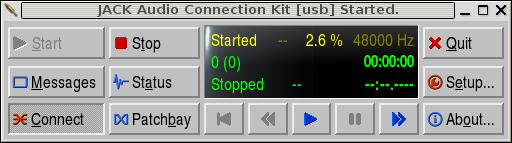
\includegraphics[width=10cm]{image200602/qjackctl-1.png}

詳細の設定を指定すると、jackdの起動オプションを細かく指定できます。

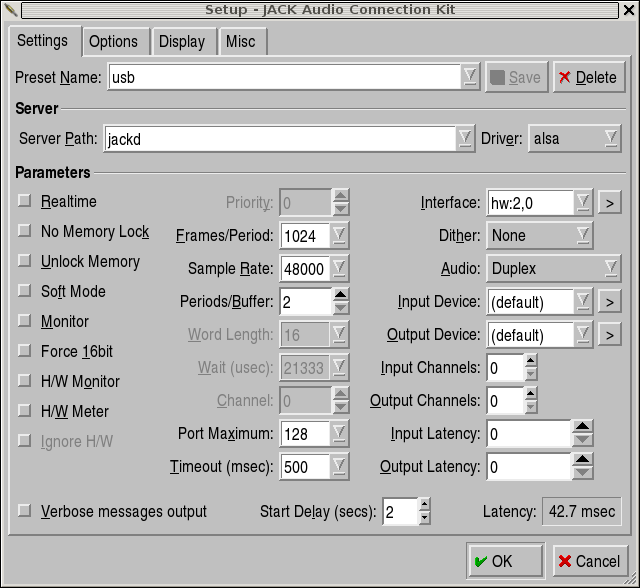
\includegraphics[width=10cm]{image200602/qjackctl-0.png}

また、コネクションパネルを開くと、jack接続の管理が出来ます。

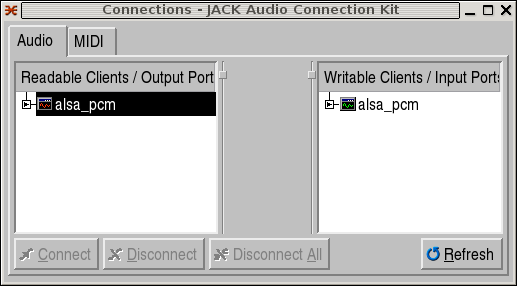
\includegraphics[width=10cm]{image200602/qjackctl-2.png}

\subsubsection{ladspa}

オーディオのエフェクトを処理するための、プラグインインタフェースです。
また、ladspa-devパッケージが存在しており、そのパッケージに含まれている
/usr/include/ladspa.h を利用することが推奨されています。
LADSPA自体がポリシーを定義していますが、Debianのladspaパッケージは、
追加で\url{/usr/share/doc/ladspa-sdk/README.Debian}にて定義されている下記のポ
リシーにしたがっています。

\url{/usr/lib/ladspa/}にパッケージが提供するLADSPAプラグインを提供するこ
と。\verb!LADSPA\_PATH! 環境変数が定義されていない場合には、
\url{/usr/local/lib/ladspa:/usr/lib/ladspa}をデフォルトの検索パスとして
利用すること。

\subsubsection{jack-rack}

apt-get install jack-rackでインストールできます。

jack接続経由でLADSPAエフェクトをかけることができ、エフェクトのパラメータ
をGUIで制御できます。

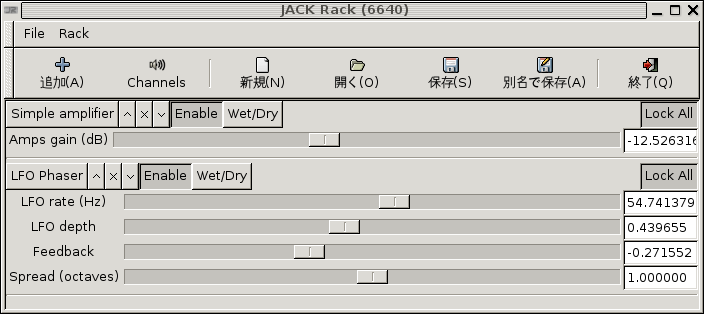
\includegraphics[width=10cm]{image200602/jack-rack.png}

\subsubsection{jamin}

apt-get install jaminでインストールできます。

jack経由で細かいイコライザーやコンプレッサーの設定が出来るツールです。
レコーディングの最終段階のファイナライズに便利そうです。

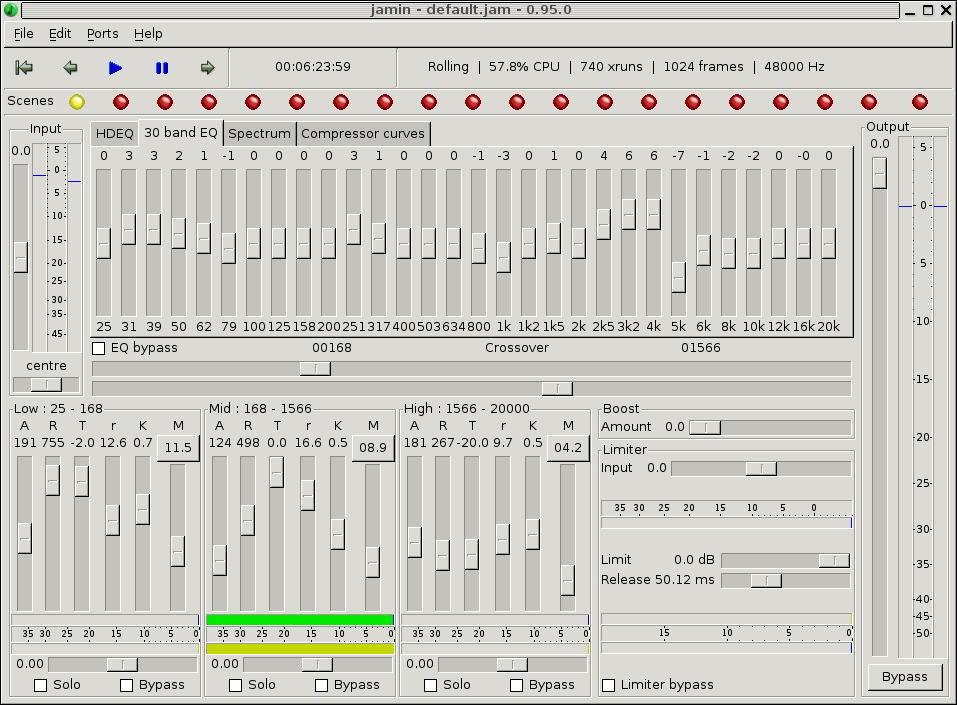
\includegraphics[width=10cm]{image200602/jamin.png}

\subsubsection{jackbeat}

apt-get install jackbeatでインストールできます。wavファイルをリズムルー
プ用のサンプルとして利用して、単純なドラムシーケンサーとして利用できるよ
うです。

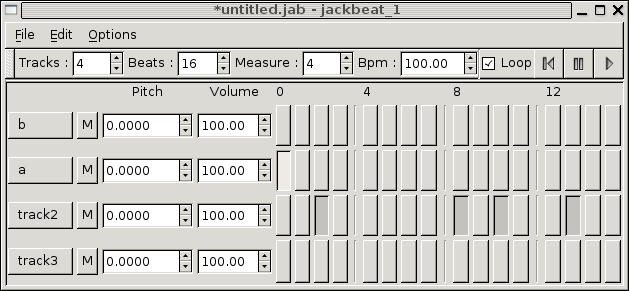
\includegraphics[width=10cm]{image200602/jackbeat.png}

\subsubsection{kluppe}

apt-get install kluppe でインストールできます。
jack経由で接続し、wavファイルをループさせることができます。

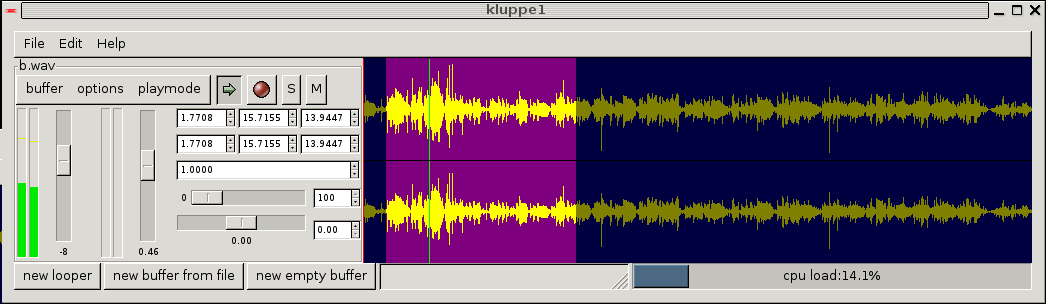
\includegraphics[width=10cm]{image200602/kluppe.png}

\subsubsection{ladcca}

LADCCAというフレームワークが存在しているようです。気づいたらlash
\url{http://www.nongnu.org/lash/} というプロジェクトにかわってしまってい
るようです。セッション管理のためのフレームワークです。jackの導入にともな
い、アプリケーションが接続できるのはよいのですが、毎回アプリケーションを
ユーザが接続する必要があります。その処理を簡便化するためのプロトコルのよ
うです。

\subsection{ソフトウェアシンセ}

MIDIの接続はALSAのMIDI接続が事実上の標準プロトコルとして利用されています。
qjackctl の接続画面にMIDI接続タブがあるので、それを利用して接続してあげればよいです。
また、aconnectというコマンドラインインタフェースがあり、それを利用するこ
とも可能です。

\begin{commandline}
$ aconnect -i -l
クライアント 0: 'System' [タイプ=カーネル]
    0 'Timer           '
    1 'Announce        '
        接続先: 15:0, 128:0
クライアント 14: 'Midi Through' [タイプ=カーネル]
    0 'Midi Through Port-0'
クライアント 130: 'Virtual Keyboard' [タイプ=ユーザ]
    0 'Virtual Keyboard'
        接続先: 129:0
$ aconnect -o -l
クライアント 14: 'Midi Through' [タイプ=カーネル]
    0 'Midi Through Port-0'
クライアント 129: 'FLUID Synth (7910)' [タイプ=ユーザ]
    0 'Synth input port (7910:0)'
        接続元: 130:0
\end{commandline}

\subsubsection{TSE3}

シーケンサエンジンのようです。KDE関連のアプリはこれを利用しているような
気がしています。どうなのよ。

\subsubsection{timidity}

ちょっとインタフェースに古めかしい感がありますが、事実上の標準のMIDIシーケンサエンジンです。MIDIデータからWAVを生成するた
めのインタフェースとして利用されています。

\subsubsection{freepats}

Debianにて、フリーのサウンドフォント集です。形式がpat形式です。timidity
から使える設定になっているようです。

sf2形式じゃないとほとんどのアプリから利用できないので意味が無い。

\subsubsection{zynaddsubfx}

apt-get install zynaddsubfx でインストールできます。

オルガン系の音やパッド系の音が結構使えます。仮想キーボードのUIがお手軽で
す。MIDI制御可能なため、vkeybdを利用して制御することなども可能です。
jack対応です。

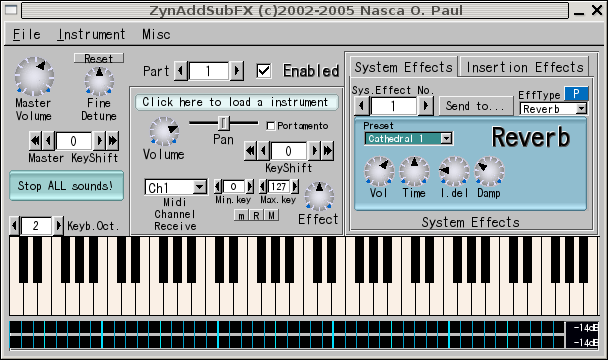
\includegraphics[width=10cm]{image200602/zynaddsubfx.png}

\subsubsection{hydrogen}

UIが優秀なのでドラムシーケンサとして活用しています。
jack 対応です。MIDI入力にも対応しているようです。

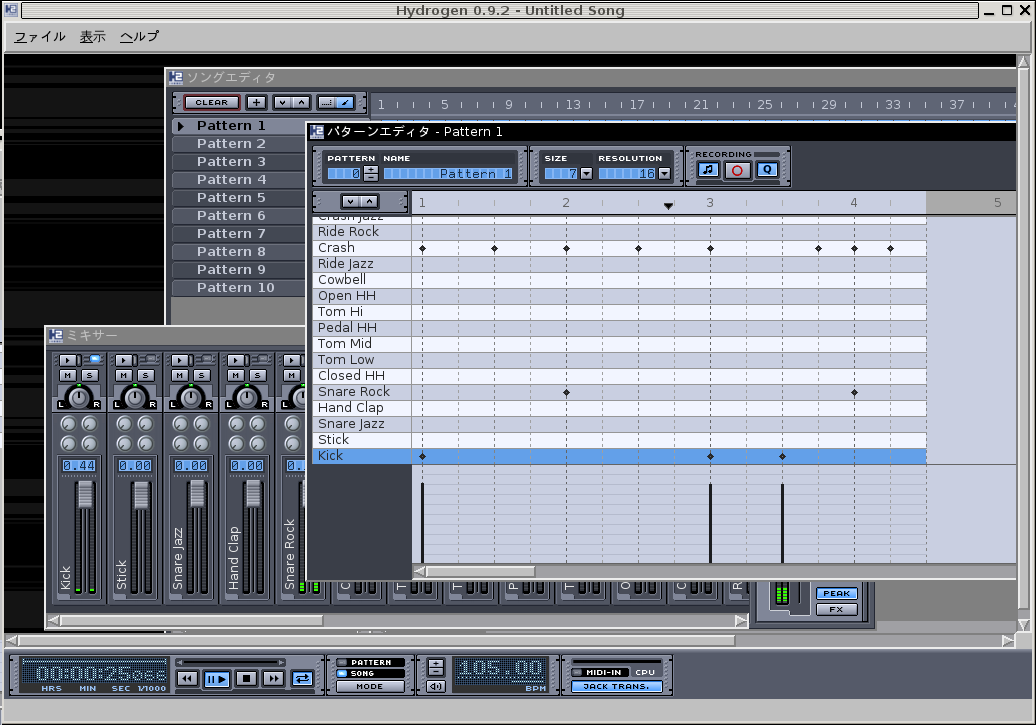
\includegraphics[width=10cm]{image200602/hydrogen.png}

\subsubsection{pd}

UIがかなり前時代的ですが、シンセをGUIで編集するという系では元祖みたいな
存在です。使い方がわからんです。誰か教えてください。

\subsubsection{beast}

GTKシンセ。これも結構頑張っています。使い方がわからんです。誰か教えてください。

\subsubsection{csound}

学術系の人々の中で長い間つかわれてきたものらしく、過去の遺産が大量にあり
ます。ちょっと学術的すぎて個人的には使っていません。誰か使い方教えてくだ
さい。

コマンドラインで操作できる、というよりむしろプログラム言語です。

方程式で波形を設計したいあなたに。

\subsubsection{vkeybd}

キーボードで操作できるMIDIキーボードです。alsaのMIDIデバイスとして動作します。
とりあえず試すのには便利です。
こいつを起動して、qjackctlで接続してあげれば他のアプリケーションがMIDI入
力にどういう反応をするのかを確認できます。

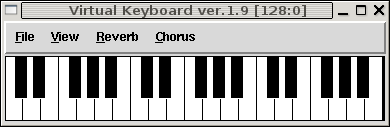
\includegraphics[width=10cm]{image200602/vkeybd.png}

\subsubsection{fluidsynth}

ソフトウェアシンセのようです。sf2形式のファイルをサポートしているようで
す。\url{http://www.hammersound.net/} などに多数のサウンドフォントが存在
していて、そのうちの適当なファイルを読み込んで利用することが出来ます。
jackへ音声を出力することが可能です。

Debian内で、sf2のファイルが見付かりません。
ウェブを探すとたくさんあるようです。

\subsubsection{qsynth}

fluidsynthを制御するGUIです。

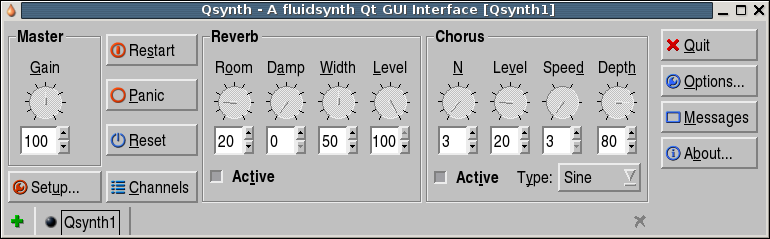
\includegraphics[width=10cm]{image200602/qsynth.png}

\subsubsection{swami}

サウンドフォント(sf2ファイル)を編集するツールです。fluidsynthを内部では
利用しています。

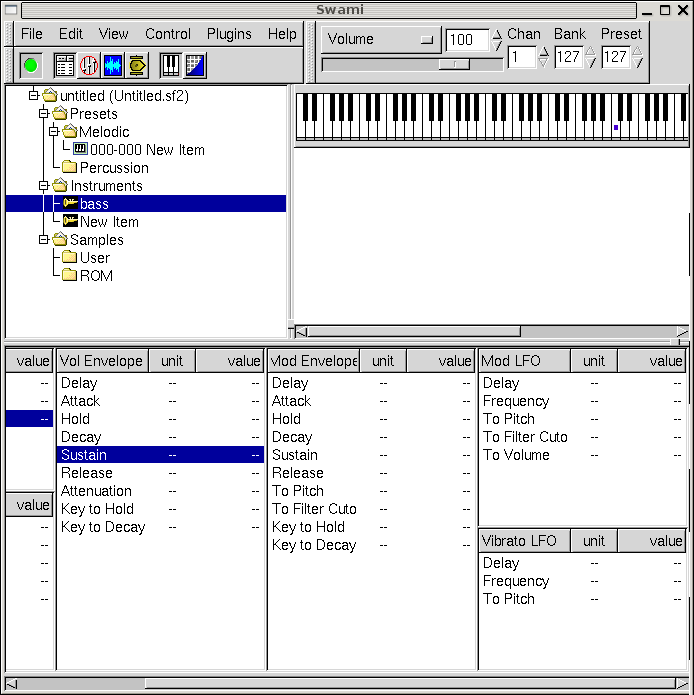
\includegraphics[width=10cm]{image200602/swami.png}

\subsection{楽譜編集}
\subsubsection{lilypond}

\TeX で楽譜を作成しよう、というパッケージ。
まともなクラシックの楽譜を作成するような作業をする際にはこれでやってました。
\TeX をがんがん使いたいあなたに。

\subsubsection{denemo}

今までは上川はこれで一小節程度の楽譜ならこちょこちょっと作成して用を足し
て来ました。キーバインドも数字で音符の長さが決まっていたり、キーの上下で
操作できます。久しぶりに見てみるとインタフェースが大幅に改善されているよ
うです。

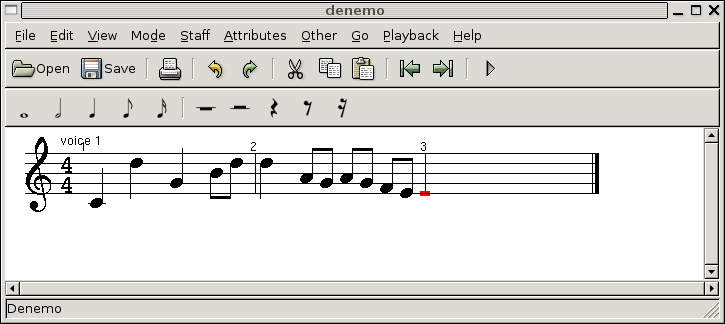
\includegraphics[width=10cm]{image200602/denemo.png}

\subsubsection{noteedit}

MIDIのインポートもできるらしい。
とりあえず楽譜を表示することはできるっぽい。

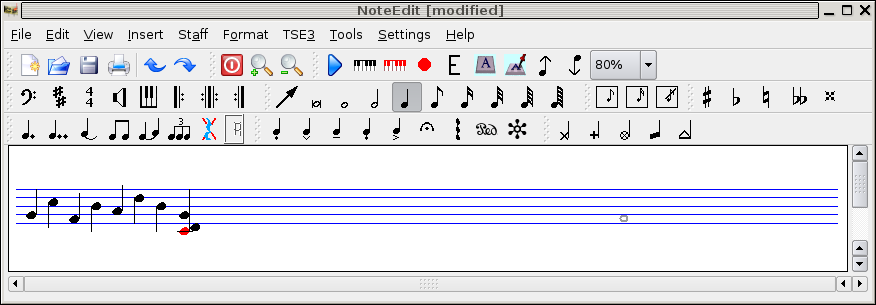
\includegraphics[width=10cm]{image200602/noteedit.png}

\subsubsection{rosegarden4}

apt-get install rosegarden4 でインストール。

一応楽譜が編集できます。ステップ録音などもできます。
デバッグメッセージが大量に出て来るのとなんだか反応が鈍い感じはします。

rosegardenという古くから何度も書き直されつづけているプログラムの最新版で
す。いまのところまともに開発されているようです。

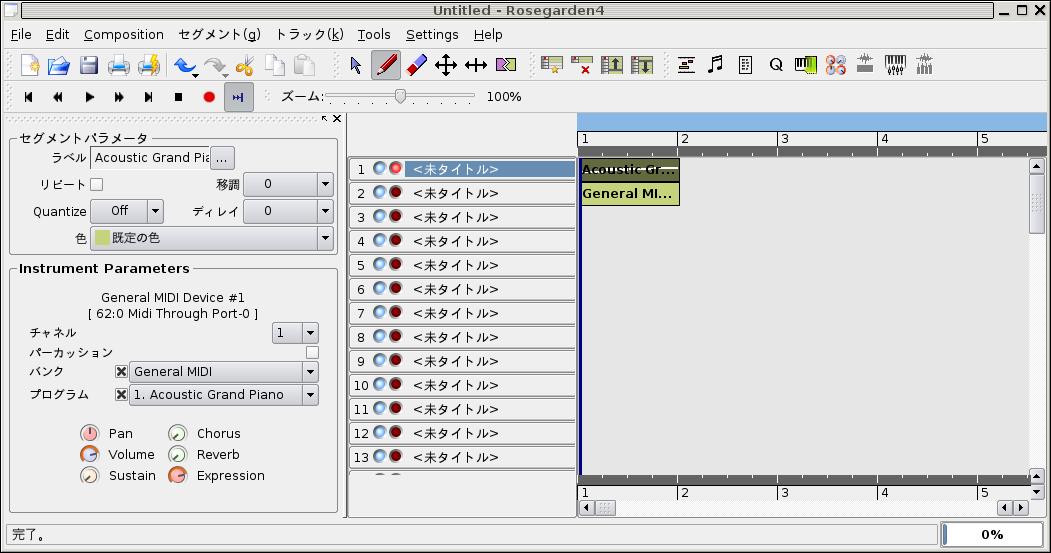
\includegraphics[width=10cm]{image200602/rosegarden4-1.png}

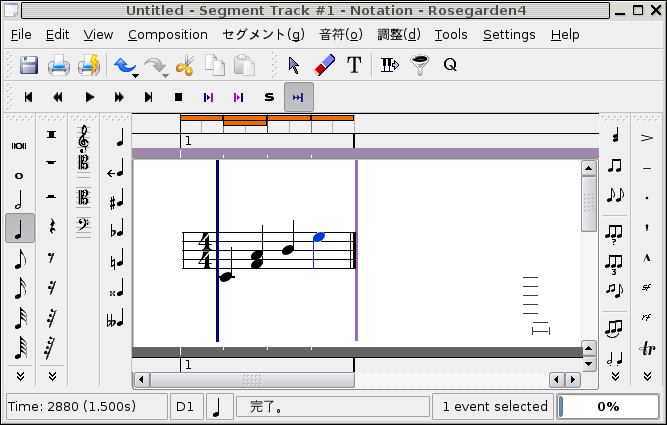
\includegraphics[width=10cm]{image200602/rosegarden4-2.png}

\subsubsection{kguitar}

apt-get install kguitarでインストール。

ギターのタブ譜を編集できるソフトウェアのようです。使い方が分からないので、
困りました。楽譜が出るはずのようですが、出てません。ギターの絵が素敵です。
MIDI入出力ができることになっているようです。

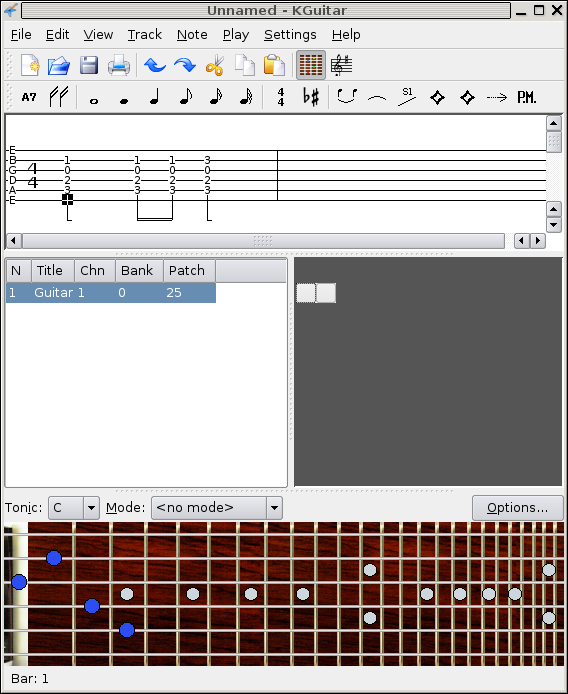
\includegraphics[width=5cm]{image200602/kguitar.png}
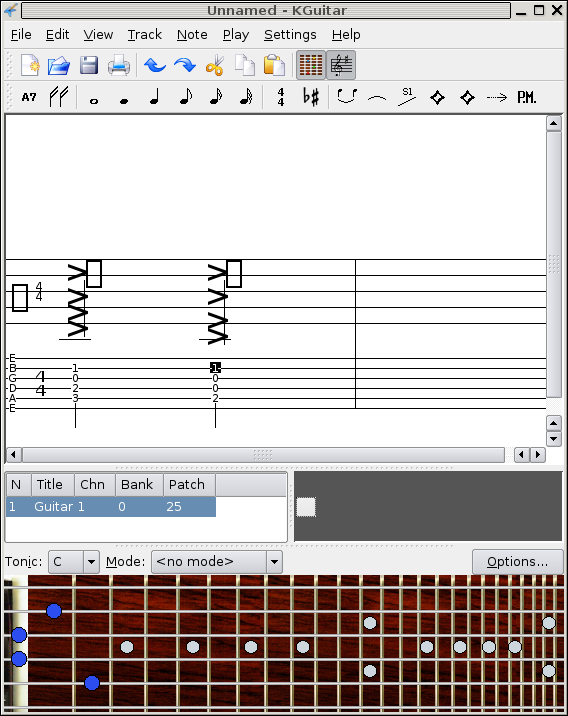
\includegraphics[width=5cm]{image200602/kguitar2.png}

\subsection{音声編集系}

\subsubsection{ecasound}

apt-get install ecasound でインストール。

コマンドラインベースで音声加工をするためのツールです。

よく使うコマンドは

音量をノーマライズする。(可能な最大の音量まであげる)\\
\begin{commandline}
$ ecanormalize in.wav
\end{commandline}
%$

in.wav にコンプレッサーエフェクトをかけて、out.wavを生成する。\\
\begin{commandline}
$ ecasound -i in.wav -o out.wav -eca
\end{commandline}
%$

とりあえず録音する\\
\begin{commandline}
$ ecasound -i alsahw,0,0,0 -o /tmp/a.wav
********************************************************************************
*        ecasound v2.4.3 (C) 1997-2005 Kai Vehmanen and others
********************************************************************************
- [ Session created ] ----------------------------------------------------------
- [ Chainsetup created (cmdline) ] ---------------------------------------------
- [ Connecting chainsetup ] ----------------------------------------------------
(eca-chainsetup) 'rt' buffering mode selected.
(eca-chainsetup) Audio object "alsahw", mode "read".
(audio-io) Format: s16_le, channels 2, srate 44100, interleaved.
(eca-chainsetup) Audio object "/tmp/a.wav", mode "read/write".
(audio-io) Format: s16_le, channels 2, srate 44100, interleaved.
- [ Chainsetup connected ] -----------------------------------------------------
(eca-control-objects) Connected chainsetup: "command-line-setup".
- [ Controller/Starting batch processing ] -------------------------------------
- [ Engine init - Driver start ] -----------------------------------------------

ここでctrl-Cで停止

- [ Controller/Processing stopped (cond) ] -------------------------------------
- [ Engine exiting ] -----------------------------------------------------------
(eca-control-objects) Disconnecting chainsetup: "command-line-setup".
- [ Chainsetup disconnected ] --------------------------------------------------
- [ Controller/Batch processing finished ] -------------------------------------
\end{commandline}
%$


\subsubsection{sweep}

apt-get install sweep でインストール。

メモリ上にwavファイルを展開するので、大きいwavファイルは編集できないです。
プリビューが優秀。ダブルクリックしたらそこから再生したりしてくれる。
こまかい波形の切りだしなどに上川愛用。
しかし、jackに対応していないなどの欠点があります。

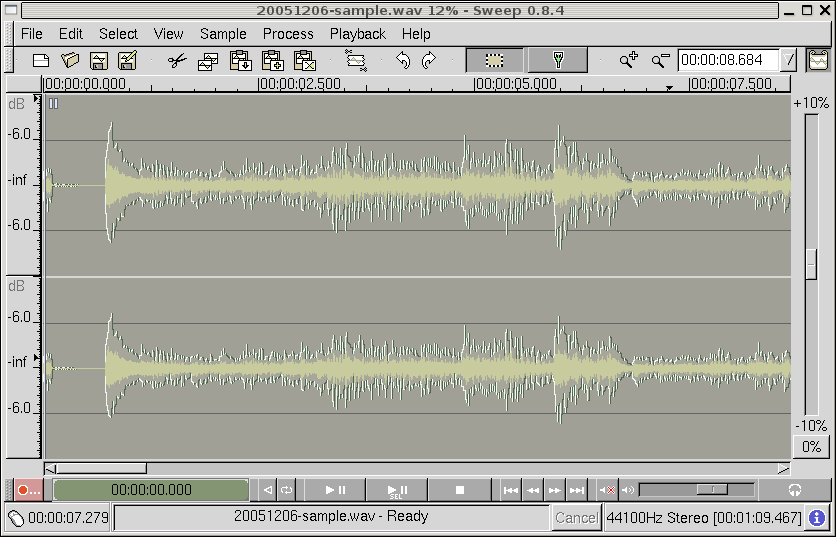
\includegraphics[width=10cm]{image200602/sweep.png}

\subsubsection{rezound}

apt-get install rezound でインストール。

サウンドの編集用のツールです。jack出力をサポートしています。

\begin{commandline}
$ rezound --audio-method jack
\end{commandline}

録音を開始する場合にはデバイスを確認されます。

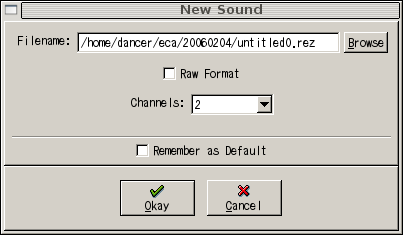
\includegraphics[width=5cm]{image200602/rezound-1.png}
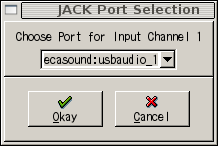
\includegraphics[width=3cm]{image200602/rezound-2.png}
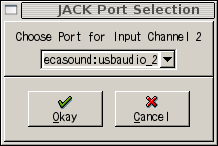
\includegraphics[width=3cm]{image200602/rezound-3.png}

録音する際にはレベルの表示もしてくれます。

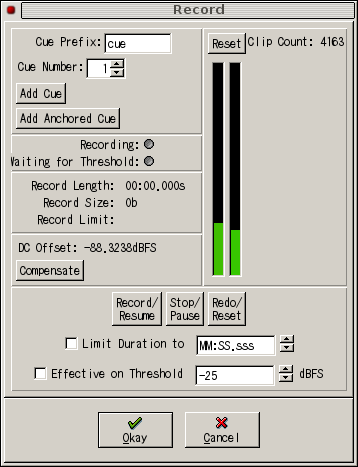
\includegraphics[width=5cm]{image200602/rezound-4.png}

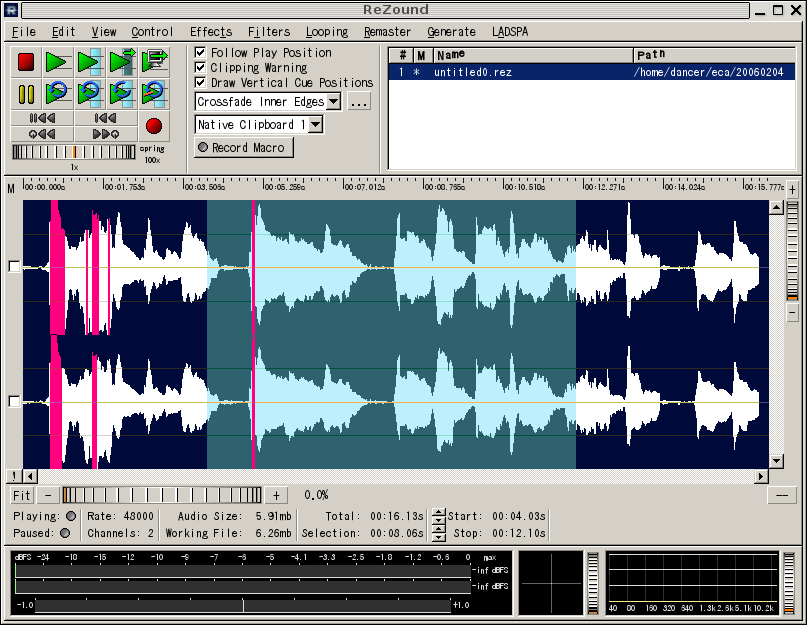
\includegraphics[width=10cm]{image200602/rezound-5.png}

入出力はjackで設定してあげます。

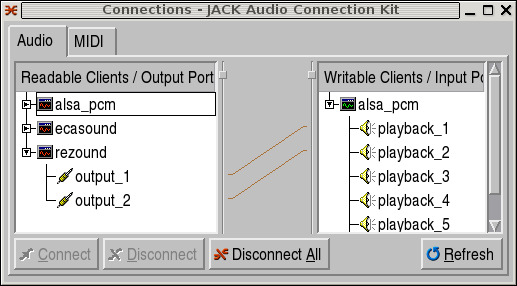
\includegraphics[width=6cm]{image200602/rezound-6.png}

\subsubsection{audacity}

apt-get install audacity でインストール。

audacityで起動。マルチトラックのオーディオ編集に最適。巨大な波形データも
メモリ上に全てをロードしようとはしないので編集できる。巨大なデータの一次
処理用には上川愛用。しかし、jackをサポートしていません。

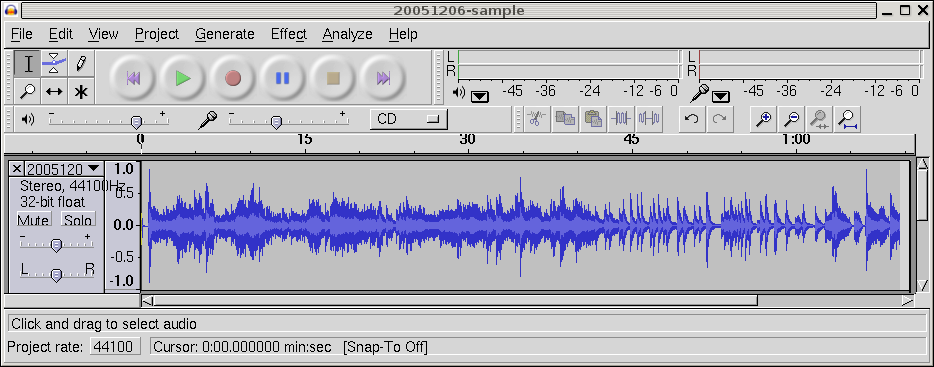
\includegraphics[width=10cm]{image200602/audacity.png}

以前は日本語インタフェースを利用しようとすると悲惨でしたが、直っているよ
うです。まだ一部問題が残っているようですが、全く使えないほどではないです。

\subsubsection{ardour}

apt-get install ardour-gtk でインストール。

マルチトラックの音声ファイルは編集できるけど、音符が編集できそうな雰囲気
は無いです。

Paul Davisという人が中心に開発していて、彼はこのためにjackとLADSPAを実装
し、Hammerfall のサウンドカードのドライバをALSA用に実装したというよくわ
からないけど凄い代物です。

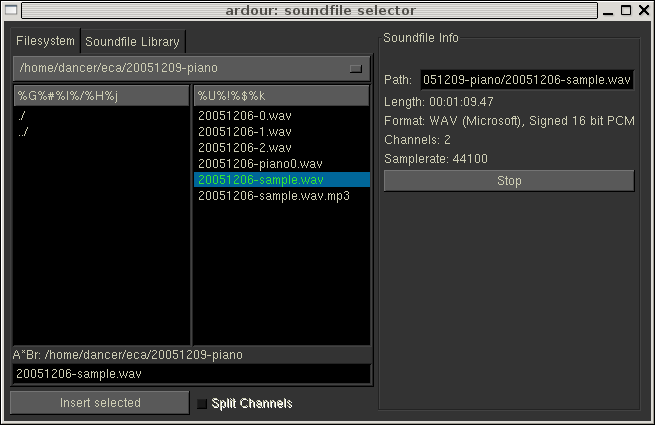
\includegraphics[width=10cm]{image200602/ardour1.png}

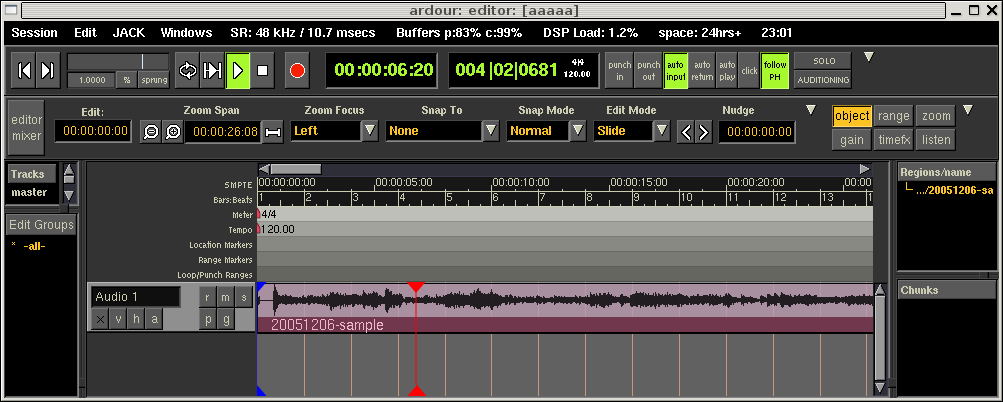
\includegraphics[width=10cm]{image200602/ardour2.png}

\subsubsection{muse}

apt-get install muse でインストール。

MIDIトラックと音声トラックが同時に扱えるようです。jackとALSA MIDIに対応
しているようです。使い方がわからず。

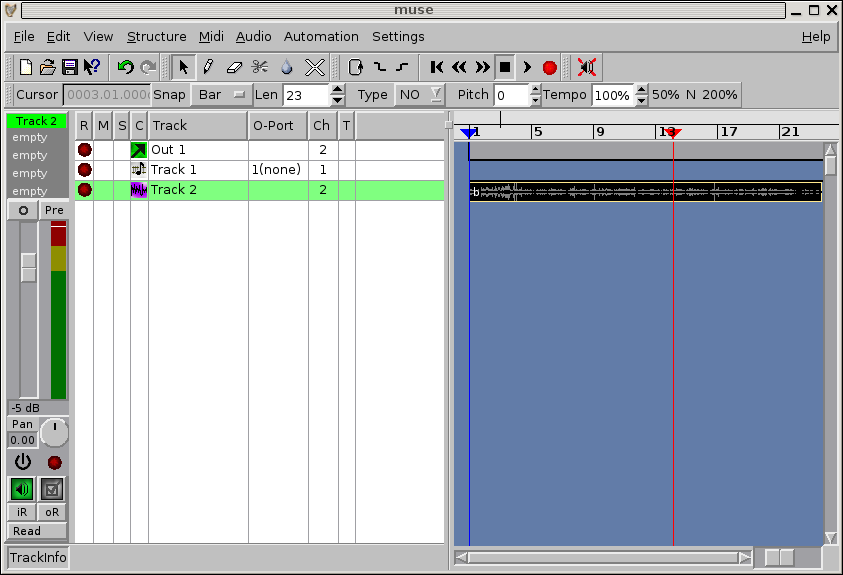
\includegraphics[width=10cm]{image200602/muse.png}


\subsubsection{snd}

音声業界でのemacsと呼ばれています。使い方がわからないです。誰か教えて下
さい。

\dancersection{Debian \TeX{}のファイル構造}{上川}
\label{sec:latexdebian1}

\TeX policyについて簡単に解説します。

\subsection{文書}
この文書は tex-common パッケージに入っている Debian-\TeX-Policy ファイル ( \url{file:///usr/share/doc/tex-common/Debian-TeX-Policy.pdf.gz})
を概訳したものです。

\subsection{用語}

用語が定義してあります。

\subsection{ファイル配置}

\TeX{}の入力ファイルのみをTEXMFツリーに配置します。
そうでないものは、/usr/share/PACKAGEに配置します。
例外として、説明のためのテキストファイルはTEXMFツリーに配置することがで
きます。

\subsubsection{パス検索とlibkpathsea/libkpse}

ファイルフォーマットなどに基づいて、TEXMFツリーの検索をするためのライブ
ラリです。
libkpathsea はあまり考えていませんでしたが、libkpseは、API/ABIを考慮したライ
ブラリです。

スクリプトからは kpsewhich, kpsepath, kpsexpand, kpsestat を利用できます。

\subsubsection{ディレクトリツリー}

配置は、\TeX ディレクトリ構造標準(TDS)に準拠する。TDSの古いバージョンに準
拠するのはバグ。TDSの新しいバージョンに依存しながらこのtex-commonパッケー
ジや \TeX の基本パッケージの十分新しいバージョンに依存していないのもバグで
す。


\begin{itemize}
 \item /usr/share/texmf-tetex/:  TEXMFDIST
 \item /usr/share/texmf-texlive/: TEXMFDIST
 \item /usr/share/texmf/: TEXMFMAIN
 \item /var/lib/texmf/: TEXMFSYSVAR
 \item /etc/texmf/:  TEXMFSYSCONFIG
 \item /usr/share/texmf-site/: TEXMFSITE
 \item /usr/local/share/texmf/:  TEXMFLOCAL
 \item texmf.cnf に指定してある  TEXMFHOME の値、もしくは環境変数として
       の値。
 \item 必須ではない: 各ユーザ用の設定ファイルディレクトリ TEXMFCONFIG, 生成されたファ
       イルのディレクトリ TEXMFVAR
\end{itemize}

検索は下から優先します。

TEXMFMAIN と TEXMFDIST の Debian での使い方はupstreamと違います。
TEXMFMAIN がバイナリと一致する必要のあるものを配置していあり、 TEXMFDIST 
はあたらしいTEXMFが配布されて上書きされるものを配置していますが、そのよ
うな配置はパッケージマネージメントシステムがきちんと動いている環境では必
要ありません。

Debianでは、TEXMFDISTをbasic \TeX packages用にしており\footnote{一部例外
あり}、
TEXMFMAINは新しいバージョンを提供したりするアドオンパッケージ用にしてい
ます。

パッケージはメンテナスクリプトの中でTEXMFHOMEを無視するように考慮すべき
です。

\subsubsection{生成されるファイル}

フォントは /var/cache/fonts におきます。
その他は  /var/lib/texmf 以下、もしくはユーザの指定したディレクトリの下
にTDSに準拠したパスに配置します。

 /etc/texmf/texmf.cnf は例外です。
管理者が編集することは意図していませんが、編集されていた場合には自動生成
ツールはその変更を尊重してください。
Debian パッケージはそのファイルは変更してはいけません。

\subsubsection{ファイル名とファイルの別バージョンのインストール}

TEXMFツリーにすでにあるファイル名と同じ名前ではファイルはインストールし
てはいけません。ただし別のアプリケーションからしか見えないサブディレクト
リにしかない場合には同じ名前でもかまいません。そういうディレクトリは
kpsewhichの --progname や --format にて得られます。

\begin{itemize}
 \item Basic \TeX packages はそれぞれ同じようなファイルを自分の TEXMFDIST 
	にインストールします。
 \item より新しいバージョンのファイルが必要な場合、TEXMFDISTにすでにある
       ファイルを自分のバージョンでおきかえることができ、TEXMFMAINに配置
       します。

       ただ、この場合、basic tex packages のメンテナに連絡
       \footnote{wishlist バグ}してください。

       新しいファイルが後方互換であるように注意してください。

       混乱をまねくため、二種類を越える種類のバージョンが共存することや、
       dpkg-divert の利用は推奨しません。
\end{itemize}

\subsubsection{ドキュメント}

パッケージはドキュメントをtexdocに提供するべきです。/usr/share/doc/texmf 
以下のサブディレクトリにファイルをインストールするか、適切なシンボリック
リンクを提供することで実現できます。

/usr/share/texmf/doc にはファイルをインストールしないでください。ここは 
/usr/share/doc/texmf へのシンボリックリンクです。

ドキュメントの代表的なドキュメントはパッケージ名に関連した名前にして、
manual.pdfやindex.htmlという名前にしないでください。
\footnote{texdoc packagenameと指定できるようにするため、これができないと
ユーザは texdoc packagename/user.dvi のようなコマンドラインを texdoc -s
keyword で検索する必要がでてきます。}

\subsection{設定}
\subsubsection{設定ファイル}

\TeX において、あらゆる \TeX の入力ファイルは設定ファイルになりえますが、設
定ファイルが多くなりすぎるのを防ぐため、 conffileやconfiguration file と
してファイルをインストールしないでください。/etc/texmf/tex には空のディ
レクトリを作成し、ユーザにどういうファイルを作成するべきかを指定してくだ
さい。

/etc/texmf/ はTDSのツリーであり、任意の設定ができます。Debian の 
tex-commonが提供する /etc/texmf/texmf.d/ などは検索対象ではないため、\TeX
の入力ファイルではないものの置場として利用できます。

\subsubsection{設定更新プログラム}

 /etc/texmf/texmf.cnf が中心の設定です。/var/lib/texmf/web2c/updmap.cfg 
がフォントの設定ファイルです。
/var/lib/texmf/tex/generic/config/language.dat がハイフネーションと言語
の設定で、 /var/lib/texmf/web2c/fmtutil.cnfにてフォーマットの生成が管理
されています。

/etc/texmf 以下のツリーからこの四つのファイルは生成されています。

updmap.cfg language.dat fmtutil.cnf についてはこれが唯一の設定方法です。

texmf.cnf は管理者によって編集可能で、変更は ucf で管理されます。

パッケージのメンテナスクリプトは直接編集せず update-texmf を利用します。
管理者もupdate-texmfを利用することを推奨します。

パッケージは設定項目を追加してよいですが、他のパッケージの設定を上書きし
ようとはしないでください。共有する設定項目は basic \TeX packages でどの
パッケージでも利用できるような値を提供させてください。もしデフォルトが不
可能であれば、そのことを関係パッケージのメンテナの間で合意をとってくださ
い。

メンテナスクリプトは、 update-updmap を --quiet オプションをつけて呼び出
して下さい。それ以外については、設定アップデートプログラムには特にオプショ
ンをつけずに呼び出して下さい。ディレクトリ構造の内部的な変更ができるよう
にするためです。

updmap.cfg を変更するパッケージは updmap-sys を呼び出す必要があります。
 language.dat か fmtutil.cnf を変更するプログラムはfmtutil-sys を呼び出
 す必要があります。
その前に mktexlsr を呼び出すのを忘れないで下さい。

\subsubsection{フォント設定}

PS type1フォントを提供するパッケージはどんな Basic \TeX package でも利用
できるようにしてください。tex-common で提供されている dh\_{}installtexを
利用してください。詳細はマニュアルページ dh\_{}installtex(1)参照。

\begin{itemize}
 \item tex-common にdepend して、Basic \TeX package には依存しない
 \item .mapファイルは TEXMFMAIN/fonts/map にインストールする。
 \item その他の必要そうなものもインストールする .pfb, .tfm, .enc, .fd,
       .sty, 文書等
 \item  /etc/texmf/updmap.d/ に 10{\it name}.cfg という名前法則でファイ
       ルを配置する。
       update-updmap が /var/lib/texmf/web2c/updmap.cfg を生成するのに利
       用される。
       \verb!# -_- DebPkgProvidedMaps -_-!を含むファイル形式で詳細は
       update-updmap(1)参照。
 \item /var/lib/tex-common/fontmap-cfg/{\it package}.list に一行一つさき
       ほどの.cfg を記述。パッケージのファイルとしてインストールすること。
 \item package.postinstと、postrm(remove/disappearを指定されたばあい)に
       て、 update-updmap --quiet, mktexlsr, updmap-sys をその順番に実行
       すること。

       (以下 dh\_{}installtex を利用すればよいので詳細な項目略)
       
\end{itemize}

\subsubsection{言語/ハイフネーション設定}

dh\_{}installtex を利用すればよいです。

必要なファイルをTEXMFMAINに配置し、
.cnf ファイルを /etc/texmf/language.d にインストール、 update-language
を呼び出すと /var/lib/texmf/tex/generic/config/language.dat が生成され
ます。

ここまでいくと、あとは
\verb!fmtutil-sys --byhyphen `kpsewhich --progname=latex language.dat`!
を呼び出すと再生成処理が行われ、利用できるようになります。
削除するときもこのコマンドです。

現状、update-languageは\LaTeX{}以外のhyphenation設定ファイルを利用してい
るものには提供されていません。

\subsubsection{フォーマット設定}

dh\_{}installtex を利用すればよいです。

fmtutil.cnf(5)に説明してある形式のファイルを/etc/texmf/fmt.d/に配置し、
 update-fmtutil を実行し、fmtutil-sys --byfmt {\it format} を実行します。
cnfファイルの最後の行に記述する {\it format}.ini が見付かった場合だけフォーマットが生成されるので、
 {\it format}.ini は conffileであってはいけません。

\subsubsection{TeXにBuild-Dependする場合のベストプラクティス}

Build-Dependするパッケージが変更した設定を必要とする場合、その設定を静的
にもつべきではありません。
もしパッケージがビルドするのに適切でない設定があるのであれば、それは通常その
設定を提供しているパッケージのバグですので、そちらを修正してください。回
避策は後々大きな問題となってかえってくる事がおおいです。

もしどうしても必要なら、設定更新プログラムの --outputdir と--add-file を
利用して生成してください。


\subsubsection{コマンドの実行とフォーマットファイル}

\TeX{}のフォーマットが必要な場合は、postinstスクリプトで実施してください。
依存するパッケージはDepends: をするだけで十分です。
フォーマットファイルの存在を確認などをすると内部構造がかわると壊れやすい
のでやめてください。

Debianパッケージは fmtutil か fmtutil-sysを常に利用するべきで、
 /etc/texmf/fmt.d/ (fmtutil-sys) にファイルを追加するか、
 fmtutil (--cnffile オプションを指定)で、ローカルのcnfファイルを更新する
 ようにしてください。

管理者は環境変数を texmf.cnf でオーバライドできます。これがpostinstのエ
ラーにつながっている例があります。環境変数はフォーマット生成前などに 
postinst で unset してください。

\subsubsection{DpkgのPost-Invokeの仕組み}

この案は没になりました。

\subsection{サンプルコード}

(省略)

\dancersection{Debian latexの現状調査}{上川}
\label{sec:latexdebian2}

まず、Debianのlatexで日本語のドキュメントを処理するための手順について確
認します。
ここでは、例としてドキュメントを準備し、そのドキュメントソースをPDFファ
イルにするまでの手順を確認します。

\subsection{platexでPDFを作成する方法}

platexはptex-binパッケージに含まれています。
日本語でかかれたtexファイルからdviファイルを生成することができます。

\begin{commandline}
 $ platex debianmeetingresume200604.tex
\end{commandline}
%$

Debian でのplatexのデフォルトは、EUCモードです。ソースファイルのエンコー
ディングは iso-2022-jp か euc-jp にしておくとよいでしょう。
SJISモードでの処理については、Debian パッケージとしてはサポート
していません\footnote{\url{http://bugs.debian.org/234547}}

\begin{center}
 \begin{tabular}{|c|c|}
 文字コード & 可否 \\
 \hline
 EUC-JP & ○ \\
 SJIS & × \\
 ISO-2022-JP & ○ \\
 UTF-8 & × \\
 \end{tabular}
\end{center}

dviファイルからPDFを作成する方法は、いくつかあります。

\begin{itemize}
 \item dvipdfmx を利用する

       毎月のDebian勉強会用の資料を処理するのに利用している方法です。

       \begin{commandline}
	$ dvipdfmx debianmeetingresume200604.dvi
       \end{commandline}
%$
 \item dvipsでPSを生成し ps2pdfを利用する

       \begin{commandline}
	$ ps2pdf debianmeetingresume200604.ps 
	mktexpk: don't know how to create bitmap font for rml.
	dvips: Font rml not found, characters will be left blank.
	$ ps2pdf debianmeetingresume200604.ps
	(結果のPDFファイルには日本語の文字がまったく表示されない)
       \end{commandline}

 \item dvi2psでPSを生成し、ps2pdfを利用する

       \begin{commandline}
	$ dvi2ps debianmeetingresume200604.dvi > debianmeetingresume200604.ps
	$ GS_LIB=/usr/share/fonts ps2pdf debianmeetingresume200604.ps
	(Ryumin-Lightが見付からない、というgsのエラーが出力され途中で停止する)
       \end{commandline}

       現状 \verb!GS_LIB! 環境変数の指定が必要になっているのと、Kochiフォ
       ントを利用しているとエラーを吐いて停止するという問題があります。
       dfontmgrを利用して、ps2pdf(gs)が利用するフォントとしてkochiフォン
       ト以外を指定する必要があります。\footnote{参考:
       \url{http://lists.debian.or.jp/debian-users/200501/msg00008.html},
       \url{http://kmuto.jp/d/index.cgi/debian/gs-esp-8151.htm} }

       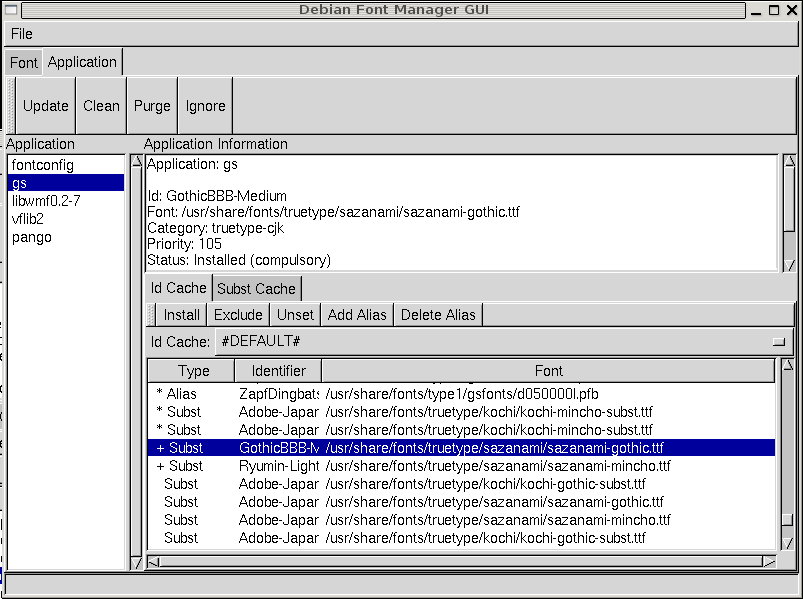
\includegraphics[width=12cm]{image200604/dfontmgr.png}

\end{itemize}

それぞれの方法にハイパーリンクやpstricksの扱いに癖があります。
たとえば、dvipdfmxの場合はhyperrefパッケージを読み込む際に、dvipdfmオプ
ションを指定してあげる必要があります。

\begin{commandline}
 \usepackage[dvipdfmx]{hyperref}
\end{commandline}

\subsection{jlatex}

jlatexは、jtex-binパッケージに入っています。
texファイルからdviファイルを生成することができます。

ただ、platex向けの既存のドキュメントをコンパイルしようとしてもエラーにな
ります。 Debian勉強会資料で利用している jsarticle.cls や ascmac.sty など
がplatex専用だからのようです。 j-articleなどを利用する必要があるようです
\footnote{jarticle は利用できるようになっている。}。また、このドキュメン
トに関してはそれ以外にも問題があり、簡単な変更では処理できませんでした。

\begin{commandline}
 $ jlatex debianmeetingresume200604.tex
! LaTeX Error: File `jsarticle.cls' not found.
(エラーがでてコンパイルできない)
\end{commandline}

\subsection{cjk-latex}

babelのCJKパッケージとして実装されており、通常のlatexを利用して日本語を
処理できるそうです。

そのままでは \texttt{/usr/share/doc/cjk-latex/examples} にあるサンプルファ
イルすらコンパイルできないので、困りものです。

参考:
\url{http://lists.debian.or.jp/debian-devel/200007/msg00150.html}

\subsection{pdfelatex}

Debianには部品が現状足りないようです。

参考:
\url{http://cise.edu.mie-u.ac.jp/~okumura/texfaq/qa/17780.html}

\subsection{multex}

パッケージをインストールしただけでは、サンプルファイルを処理してもフォン
トが一部足りないようで、表示されない文字があります。

参考:
\url{http://lists.debian.or.jp/debian-users/200106/msg00081.htm}

\subsection{lambda (omega)}

\url{http://www.fsci.fuk.kindai.ac.jp/kakuto/soft.html}、
\url{http://cise.edu.mie-u.ac.jp/~okumura/texfaq/japanese/}などを参考に
してみてください。現状、実用的に既存のドキュメントをそのまま処理できるよ
うな形式ではないことがうかがえます。



\dancersection{一年間Debian勉強会をやってみて}{上川}
\label{sec:uekawa}
%% 上川の記事はここから 

この記事の目的は、終ってからだと忘れてしまいそうだし、最中だといそがしく
ていっぱいいっぱいなのでどこにも記録されずに忘れ去られてしまいそうな事項
についてメモをしています。

希望としては、ここに書いてある内容をみて、今後のミーティングの運営の手伝
いを人に頼めるようになればよいなと思っています。

\subsection{月例のDebian勉強会のワークフロー}

2005年、Debian勉強会を毎回実施する際に利用したワークフローを紹介します。今後の勉
強会などの参考にできるかと思い、記録します。

参加者規模、10名から20名程度でした。
予算規模は、宴会を含むと一回5万円から10万円程度です。
宴会を含まないのであれば、多くて1万円くらいでした。(\tbref{tab:yosan})

\begin{table}[ht]
 \caption{予算概算}\label{tab:yosan}
 \begin{center}
  \begin{tabular}{|c|c|}
  項目 & 予算 \\
 \hline
  部屋代 & 1500 \\
  コピー代 & $ 300 \times \texttt{人数} $ \\
  宴会代 &  $ 5000 \times \texttt{人数}$ \\
  \end{tabular}
 \end{center}
\end{table}


\subsubsection{1年前}

開催者側のスケジュールの確保。
上川は一年前にだいたいその年のスケジュールを決めています。

\subsubsection{2ヵ月前}

会場の予約確保、開催を決断。

\subsubsection{1ヵ月前}

この時期にすくなくともテーマの設定をします。
講師の確保をしておきます。資料の作成開始をしておかないと間に合わないで
しょう。目処がつきそうだったら、開催のスケジュールを対外的に公表します。
参加者にスケジュールの調整をお願いします。

\subsubsection{1週間前}

宴会の会場選定などを実施します。
大体、資料作成のデッドラインです。
リマインダーの送付をします。

\subsubsection{2日前}

事前課題の文書を事前資料に転記したり、最終的な文書の校正。
この時点で資料の印刷用の最終版が作成。

宴会の人数確定。
宴会予約。

ただ、二日前に選定するとなると場所が限られる場合が多いので、本当はもっと早い時期がよ
いです。一般には、確定が早ければ早いほど予約は安くすみます。
二日前になっても参加できるかどうかわからないという人がいますが、
そういう人の対応は難しいです。
店の柔軟な対応に期待するか、コストをかけるしかないです。
しかし、12月10日の宴会も前日で予約できたのであれば、実は当日に急に開催決
定するとかいうのでさえなければ何とかなる物なのかもしれないです。

\subsubsection{1日前}

資料の印刷をします。
Kinko'sにすべてを依頼する場合は場合にもよりますが、半日くらいは見込む必要があります。
自分で全部するとしても量によりますが、一時間は見込む必要があります。

Kinko's にすべてを依頼する場合、部数が少ないとかなり割高になります。
\footnote{A3の紙にA4を面付けしてもらい、なかとじホッチキス製本にすると
ホッチキスだけで150円/冊になります。コピーが一面14円程度になります。
結果として、一冊450円程度になる。会費を500円しか徴収しないことを考えると、会場費用を
考えると確実に赤字になってしまうので注意。}

\subsubsection{当日}

資料をもっていきます。
司会をします。
適当にもりあがります。

宴会も実施します。
2005年は、講師は無料で宴会、ということで運営しました。
ただ、ときどきそれでは予算が苦しい場合も多々ありました。
なぜか宴会に来ているのに現金をもっていない人とかの扱いには苦慮します。

予算は、ほぼ確実になんらかの理由でのキャンセルが発生するため、
余裕を20%くらい確保できていないと赤字になります。
\footnote{
回避策としては、来ない人から徴収するとかいう案も可能性としてはありますが、
来ない人から徴収するということは暗黙に開催者が次回その来ない人から徴収す
る分について肩代りする、ということを意味するため、オーバヘッドが発生する
ことを忘れてはならない。
}


\subsection{JDMCのような大きなイベントのワークフロー}

Japan Debian Miniconfはまだまだこれから育って行くようなイベントです。
今回蓄積できたノウハウだけで今後もうまく開催できるとは思っていません。
ただ、今回イベントを開催する上で重要でたりなかった点を列記していきます。

\begin{itemize}
 \item 連絡先を明確にする。
 \item 緊急時に判断をできる人を明確にする。
 \item 連絡網を整備する。
 \item ディスカッションができて、そこで決定した事項が合意したとみなせる
       環境をきめてしまう。たとえばIRC。
\end{itemize}

一人ではかぶりきれない責任もあるため、
大きなイベントでは、本気で責任をもって開催したい、と思っている人が複数
いる必要があります。

会議の内容をログに残して全員に周知させる係の人が必要です。
理想としては、実働部隊と分けられればわけたほうがよいです。
JDMCでは、ほとんど矢吹さんだけに情報が集中していたはずで、
メーリングリスト上ではながれていない情報が多数ありました。
もしかすると検討する余裕がなかった項目も多数あったかもしれません。

また、メーリングリストで流れる情報は時系列なので、
現在のステータスを一覧で把握できないです。
タスクトラッキングが重要になります。

また、全員がどういう方法で情報交換をするのかという点について同意が必要で
す。メールで主要な情報交換はなされたのだが、一部の主要メンバーの人達がメー
ルをほぼ全く読んでいなかったという問題がありました。


\subsubsection{2年前}
参加者が稼動できるように日程を確保します。
スポンサーにあたりをつけはじめる。
マネージメント層に交渉します。
それとなく開催できそうな雰囲気がただよっていることを確認します。

\subsubsection{1年前}

一年前か、半年前くらいの時期にスポンサーの予算が大体確定するはずです。
講師に関しての予定、参加者の人数、プログラムの大体のイメージが決まってい
る必要があります。

初の企画でないのなら、前年度のイベントに参加して運営側で何がおきるかを明確にして、
会場のサイジングなどをする必要があります。

スポンサーに関しては、通常スポンサーから資金が提供されるのはイベントが終
了した後です。そのため、事前に当面必要な運転資金をどう確保するのかとい
うのも検討しておく必要があります。

また、赤字になることが見込まれるのであれば、計画を中止するという選択も必
要です。

\subsubsection{6月前}

会場を確保します。
宴会場を確保します。

予約システムを整備し、広報します。
広報は下記を想定しています。

\begin{itemize}
 \item マスメディアへの広報
 \item IRCなどのくちこみ。
       \verb!#debian-devel@opn!など
 \item Blog
 \item DWNへの投稿
 \item メーリングリスト, debian-devel@debian.or.jp,
       debian-users@debian.or.jp, debian-devel@lists.debian.org
 \item Mixiなどのソーシャルネットワーク
 \item Slashdotへ たれこむ
\end{itemize}

また、GPGサイン会などを実施するのなら事前に充分に準備、広報する必要があ
ります。

\subsubsection{1月前}

宴会場の確保、決定が必要です。

参加者の登録が確定しているくらいが本当は好ましいです。
人数が足りないのであればがんばってかきあつめるなどのアクションをとります。

ロジスティックの計画があるので、この時点での人数の把握は重要。

\subsubsection{7日前}

宴会場に連絡して、大体の人数を調整。

\subsubsection{2日前}

宴会場との調整、当日の人数のより確度の高い情報を提供。

\subsubsection{当日}

参加者の出欠確認

参加費用の集金を実施します。

スポンサー企業からの提供物を提供します。スポンサーのグッズとかです。

\subsubsection{事後}

スポンサー企業への報告を作成します。
結果報告書を書き上げます。

参加者の報告をまとめてもらいます。来年のイベントに繋げるために重要です。

次回への検討をはじめます。

\subsubsection{参考文献}

いろいろと他のイベントの報告などもあります。参考になりそうなものを列挙し
ます。

\begin{itemize}
 \item
      Joey の LinuxTagレポート
      \url{http://www.infodrom.org/~joey/Vortraege/2005-06-24/index.html}
 \item
      Joey の LinuxTag感謝状
      \url{http://www.infodrom.org/~joey/log/?200512020951}
 \item
      Debconf5 Final Report
      \url{http://lists.debian.org/debian-devel-announce/2005/12/msg00001.html}
      
\end{itemize}

\subsection{やった内容}

やった内容はけっこういろいろありました。
最初は一般的なうけをねらったものもありましたが、
全体的には技術的な内容を主としています。

\begin{itemize}
 \item 毎月のクイズ
 \item 最初の数回はグループワーク
 \item バックアップリストアについて
 \item ネットワーク監視
 \item reportbugの使い方
 \item debhelper
 \item Social Contract
 \item po-debconf
 \item lintian/linda
 \item dpkg-cross
 \item dsys/update-alternatives
 \item debian-installer
 \item dpatch
 \item toolchain
 \item ITPからアップロードまでの流れ
 \item debconf 2005 参加報告
 \item Debian JP webの改革
 \item debconf の使い方
 \item apt-listbugs
 \item debbugs
 \item dpkg-statoverride
 \item Debian Weekly News 日本語翻訳のフロー
\end{itemize}

来た人数は\tbref{tab:count}にあるような数字です。正確な記録は実は残っていないような気が
しています。議事録をあさればわかるのかもしれません。

\begin{table}[ht]
 \caption{参加人数(概算)}\label{tab:count}
 \begin{center}
  \begin{tabular}{|l|c|}
   & 人数 \\
 \hline
   2005年1月 & 21 \\
   2005年2月 & 10 \\
   2005年3月 (早朝)& 8\\
   2005年4月 & 6\\
   2005年5月 & 8\\
   2005年6月 & 12\\
   2005年7月 & 12\\
   2005年8月 & 7\\
   2005年9月 & 14\\
   2005年10月 & 9\\
   2005年11月 & 8\\
   2005年12月 & 8 \\
  \end{tabular}
 \end{center}
\end{table}


\subsection{おきたトラブル}

勉強会を毎月開催する上で発生したトラブルを紹介します。
\tbref{tab:trouble}です。数字はどれくらいの確率でおきたような気がしてい
るかというのをなんとなく気分的に定量的に書いてみました。

\begin{table}[ht]
 \caption{発生トラブル}\label{tab:trouble}
 \begin{center}
  \begin{tabular}{|l|c|}
   イベント & 発生率 \\
   \hline
   パソコンが盗まれる &  10\%\\
   家が水没する &  10\%\\
   病気で倒れる &  20\%\\
   〆切におくれる &  20\%\\
   なぜか講師のひとと前日まで音信不通 &  10\%\\
   20分くらいまえに連絡してきて、来れないという参加予定者がいる。&  100\%\\
   何も連絡なく来ない人がいる &  100\%\\
   なぜか赤字 &  40\%\\
  \end{tabular}
 \end{center}
\end{table}


\subsection{できた内容}

事前課題により事前にawarenessを向上しました。
いろいろと知らないことを積極的に調べることにより講師がその分野に詳しくな
るという副作用があります。
調査して文章を書いている過程でバグが気に入らないので、バグが直る、という
ことを若干期待しています。

勉強会をクイズではじめてみんなで発言することにより場を和ませることができ
たか?と思っています。クイズは、全員に紙で配布して解いてもらわないと、順
番にあてる形でやると、一部の回答している人だけが集中して、その他の人が当
事者意識をもたないという問題があります(JDMCでの失敗)。
紙を毎回印刷するコストは大きいですが、それなりに効果もあります。

終ってからの blog へのリンク、議事録の掲載についてはあまり反響が無いです。
事前資料のPDFについてはいろいろとblogとかをみているとコメントがあったこ
ともありますが、そちらも反応はあまりないようです。
見られているのかどうか不明です。PDFファイルだからでしょうか?

勉強会の資料を半年分まとめて書籍のような形式にして、
Debian 勉強会資料ということで、コミックマーケットにて販売してもらう、とい
う試みをしています。これは、以前Debian関係の話題が豊富にはいっていた
「Debuan BNU/Linux 不徹底入門」という同人誌があったのですが、それが廃刊
になったため、その代替となれることをめざしているためです。

\subsection{今後やりたいこと}

今後は事前の打合せをもっと密にしたいと考えています。

IRCの debianjp チャンネルで偶然いたメンバーで、なんとなく打合せをする、
ということはできていました。
しかし、最初のころは事実上打合せは上川が電話で呼び出してどっかの飲み屋で
する、という手法をとっていました。
後半は時間の都合で、ほとんど打合せができていなくて、前回の勉強会の後の飲
み会で決定した内容そのままで次の勉強会にのりこむ感じでした。

事後の処理をなんとかしたい、と考えています。
開催した結果をもっと参加していない人にもわかるように効率よくアウトプット
できないだろうか、と思っています。

他の人が参加したいと思えるようなアウトプットが出せないだろうか、と考えて
います。
勉強会自体にDebian関係者が参加したい、と思えるようになることと、
Debianにこれから入る人達が参加したい、と思えるようになることが必要だと思
います。

来年の提案として
システムの構築報告、動作検証、というのはどうだろうか。
「この組合せはできるだろう」、という組合せに関して、
連係はこうやってできる、ということを報告していけば、
多くの人がその動作を確認できるようになり、
問題も解決していけるでしょう。
Debianユーザの勉強会というのはそういう形になるのではないでしょうか。

Debian勉強会以外では、おそらく開発に必要な情報についてまとめて情報収集できる場というのが存在しないため、
開発に必要な情報については継続してやりたいと考えています。
ただ、2回に一回くらいはそういうユーザよりの情報の検証にあててもよいだろ
うと考えています。

また、勉強会でいいっぱなしではなく、勉強会の結果何かが起きる、というようにした
い。
メンテナがバグトラッキングシステムにバグをファイルします、というように宣
言して、毎月その進捗を報告する、という内容にしてみてもよいかな、と思って
います。



\dancersection{Debian勉強会の事前資料の作成はどうやってやったか}{上川}

\subsection{作成ツール}

作成のデータ共有にはaliothのcvsを利用しました。

データの編集は上川はemacs+yatex+whizzytexで実施しました。
\LaTeX 処理系としてplatexを利用しました。
PDFの作成は、dvipdfmxを利用しました。

プリビューはdviファイルはadvi、PDFファイルに関しては、xpdfを利用しました。 

上川の編集環境はDebian sidで、常に開発中の環境だったので、
その時期において動かないツールというのもたまにあり、それなりに大変でした。
原稿の編集中には \texttt{apt-get dist-upgrade}しないように自制していまし
た。

\subsection{\LaTeX ソース}

事前資料は\LaTeX で作成しました。
作業は大きく3種類ありました。

\begin{itemize}
 \item クイズの作成
 \item 参加事前課題の作成
 \item 勉強会のネタの作成
\end{itemize}

\subsubsection{クイズ}
クイズについては、 \LaTeX のマクロでクイズを作成できるようにして、それを利
用して本文を作成しました。

\LaTeX のソースに下記のように記述すると、

\begin{commandline}
 \santaku{問題文}{回答A}{回答B}{回答C}{回答}
\end{commandline}

下記のような出力がでるようになりました。

%\begin{screen}
 \santaku{問題文}{回答A}{回答B}{回答C}{解答例}
%\end{screen}

また、その出力を latex-beamer\footnote{\LaTeX でプレゼンテーションを作成す
 るためのスタイル}
 で処理をして、プレゼンテーション形式になるようにしました。
2005年10月以降、勉強会当日は、それを利用して回答を提示するようにしました。

\subsubsection{参加事前課題}

メールにて参加者からplain textできたものを気合いで\LaTeX になおしました。
\LaTeX で使えない文字というのがあるので、それをエスケープすることと、
構造文書については、構造を\LaTeX 用に書き直すという手順が必要です。

例えば、下記のような文章は

\begin{commandline}
□ これについて

こんなことをしてみた

□ あれについて

あんなことをしてみた

□ それについて

いっぱいしてみた

\end{commandline}

itemize環境を利用して下記のような文書になります。

\begin{commandline}
\begin{itemize}
 \item{これについて} こんなことをしてみた
 \item{あれについて} あんなことをしてみた
 \item{それについて} いっぱいしてみた
\end{itemize}
\end{commandline}

\begin{itemize}
 \item{これについて} こんなことをしてみた
 \item{あれについて} あんなことをしてみた
 \item{それについて} いっぱいしてみた
\end{itemize}


\subsubsection{勉強会のネタ}

講師の方に直接 \LaTeX で文書を書いてもらいました。
CVSレポジトリはalioth.debian.orgでホスティングしてもらったので、
そこに共同開発者という形で参加してもらいました。

\LaTeX のスタイルはほぼそのまま jsarticle を採用しています。
ただ、セクションのはじめの部分だけはみかけを派手にしようとして
dancersection というマクロを作って独自に定義しています。
各筆者は dancersection 以下に適当に subsection を作って
文書を作成する、というルールになっています。

\begin{commandline}
\dancersection{一年間Debian勉強会をやってみて}{上川}
\label{sec:uekawa}
%% 上川の記事はここから 
\subsection{セクションの名前 }

文章がだらだらと続く

\subsubsection{セクションの名前 }

.
.
.

\subsection{セクションの名前 }
.
.
.

\end{commandline}

\subsubsection{URLやメールアドレスの処理}

\verb!\url{http://url...}! というように表記しています。
また、メールアドレスも環境を定義するのが面倒なので、そのまま
\verb!\url{メール@アドレス}!という形式にしています。

\subsubsection{特殊文字の処理}

\LaTeX でエスケープが必要な文字については\tbref{tab:tokushu}のように対処しています。
\begin{table}[ht]
 \caption{特殊文字}\label{tab:tokushu}
 \begin{center}
  \begin{tabular}{|c|c|l|}
  文字 & 名称 & 表記 \\
 \hline
 \~{ } & チルダ & \verb!\~{ }! \\
 \underline{ } & アンダーライン & \verb!\underline{ }!\\
 \# &ハッシュ& \verb!\#!\\
 \% &パーセント& \verb!\%!\\
  \end{tabular}
 \end{center}
\end{table}


\dancersection{Debconfで開催された会議概要}{岩松、矢吹、上川}
\label{sec:debconf6}

2006年の Debian Conference はメキシコで開催されました。
日本からは、武藤さん、上川さん、g新部さん、矢吹さん、岩松が参加しました。
\subsection{Debian Conference の過去の経緯}

\begin{minipage}{0.5\hsize}
Debian Conference\footnote{\url{http://debconf6.debconf.org/}} は Debian 
の開発者たちが一同に介するイベントです。通常顔をあわせることのないメンバー
たちが一同に介し友好を深め、技術的な議論を戦わせます。過去の開催履歴を見
てみると右のようになります。
\end{minipage}
\begin{minipage}{0.5\hsize}
\begin{center}
{\footnotesize
 \begin{tabular}{|c|c|c|r|}
 \hline
 年 & 名前 & 場所 & 参加人数 \\
 \hline
 2000 & debconf 0 &フランス ボルドー & \\
 2001 & debconf 1 &フランス ボルドー & \\
 2002 & debconf 2 &カナダ トロント & 90名 \\
 2003 & debconf 3 &ノルウェー オスロ & 140名 \\
 2004 & debconf 4 &ブラジル ポルトアレグレ &  150名 \\
 2005 & debconf 5 &フィンランド ヘルシンキ & 200名 \\
 2006 & debconf 6 &メキシコ オアスタペック & 300名 \\
 \hline
 \end{tabular}
}
\end{center}
\end{minipage}


\subsection{会場}

\begin{minipage}{0.5\hsize}
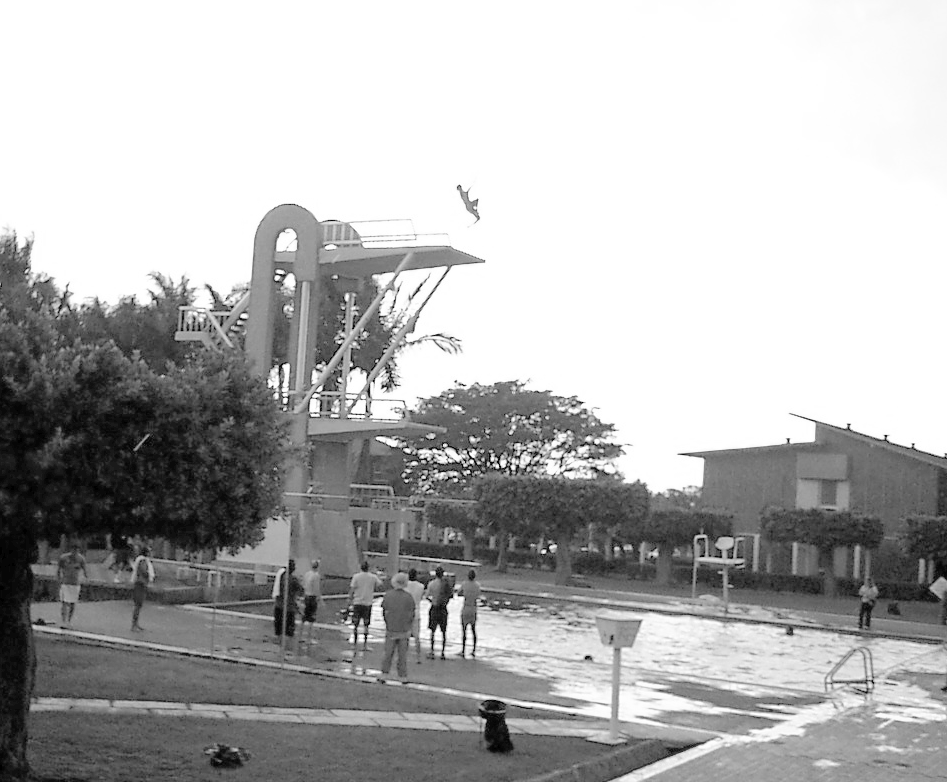
\includegraphics[width=0.9\hsize]{image200606/jumping.png}
\end{minipage}
\begin{minipage}{0.5\hsize}
今回の Debian Conference の会場は Mexico City から車で2時間ほど走ったと
ころにある Oaxtepec というリゾート地です。オリンピックに使われた会場をそ
のままリゾートホテルにしているような雰囲気です。Centro Vacacional IMSS
Oaxtepec という会場でした。プールと10mのとびこみ台などが完備されており、
ハック以外にもいろいろとできる感じがしていました。

\end{minipage}

\subsection{会の規模}

会議室は150人程度入れる会議室が準備されていました。 Hacklab として、二つの部屋
があり、それぞれには50人づつくらいが入れるようになっていたようです。

今回の参加者は登録記録によると 300 人だそうです。国別の表を次にまとめま
した
\footnote{\url{http://lists.debconf.org/lurker/message/20060518.203936.b6df5950.en.html}} 
。

今回のネットワークは 192.168.x.x で、23ビットでした。大体500台位接続でき
る計算になりますが、全員接続していた時間帯において DHCP サーバから IP が
とれなくなっていました。これは DHCP のプールを使い切っていたのではないでしょ
うか?ネットワーク自体は近くのネットカフェから無線 LAN で引っ張っていま
した。さらにこの無線 LAN をハックラボとセッションをするための会議室(通
称:タワー)を LAN でつなぐために屋根づたいで有線を引っ張っていました。

セッションも多数ありました。全体として、
参加した人数の概要も表にまとめました。

\begin{minipage}[t]{0.3\hsize}
 {\scriptsize
\begin{center}
 \begin{tabular}[t]{@{\vrule width 1pt}c|r@{\ \vrule width 1pt}}
\hline
国 & 人数 \\
\hline
 MEXICO & 144 \\
 UNITED STATES & 48 \\
 VENEZUELA & 31 \\
 GERMANY & 29 \\
 UNITED KINGDOM & 17 \\
 ITALY & 17 \\
 SPAIN & 16 \\
 EL SALVADOR & 16 \\
 BRAZIL & 16 \\
 FINLAND & 15 \\
 FRANCE & 9 \\
 COLOMBIA & 8 \\
 ARGENTINA & 8 \\
 NORWAY & 6 \\
 JAPAN & 5 \\
 CANADA & 5 \\
 BELGIUM & 5 \\
 PERU & 4 \\
 BELIZE & 4 \\
 SWITZERLAND & 3 \\
 SWEDEN & 3 \\
 NETHERLANDS & 3 \\
 INDIA & 3 \\
 GREECE & 3 \\
 CAMEROON & 3 \\
 AUSTRIA & 3 \\
 AUSTRALIA & 3 \\
 RUSSIAN FEDERATION & 2 \\
 ROMANIA & 2 \\
 NIGERIA & 2 \\
 BOSNIA AND HERZEGOVINA & 2 \\
 BOLIVIA & 2 \\
 UKRAINE & 1 \\
 NEW ZEALAND & 1 \\
 LATVIA & 1 \\
 KENYA & 1 \\
 ISRAEL & 1 \\
 IRELAND & 1 \\
 INDONESIA & 1 \\
 GUINEA & 1 \\
 GUATEMALA & 1 \\
 GAMBIA & 1 \\
 EGYPT & 1 \\
 CZECH REPUBLIC & 1 \\
 CUBA & 1 \\
 CROATIA & 1 \\
 CHINA & 1 \\
 CHILE & 1 \\
 CAMBODIA & 1 \\
 BANGLADESH & 1 \\
\hline
 \end{tabular}
\end{center} 
}
\end{minipage}
\begin{minipage}[t]{0.7\hsize}
 \begin{center}
 {\scriptsize
 \begin{tabular}{|l|l|p{20em}|r|}
\hline
日 & 時間 & タイトル & 参加人数 \\
\hline
 2006-05-14 Sunday & 11:00-11:45 & Welcome by DebConf Organizers &  50 \\
 2006-05-14 Sunday & 12:50-13:35 & wiki.debian.org BoF by Joey Hess &  29 \\
 2006-05-14 Sunday & 12:50-13:35 & OpenSolaris, Java dn Debian:  can we be friends? Simon Phipps, Alvaro Lopez Ortega &  92 \\
 2006-05-14 Sunday & 15:20-16:05 & Advanced tools for wasting time by Enrico Zini &  90 \\
 2006-05-14 Sunday & 18:00-19:00 & Multithreading:  Why and how we should use it by Ben Huthcings &  30 \\
 2006-05-15 Monday & 10:05-11:45 & Python BoF by Andreas Barth et al &  28 \\
 2006-05-15 Monday & 10:05-10:50 & Embedding Debian by Wookey &  31 \\
 2006-05-15 Monday & 11:00-11:45 & Topper: An Open Source Driver Framework by Maxim Alt and Dario Rapisardi &  59 \\
 2006-05-15 Monday & 11:55-12:40 & Ubuntu annual report by Mark Shuttleworth &  122 \\
 2006-05-15 Monday & 12:50-13:35 & i18n Infrastructure AdHoc Session I by Christian Perrier &  ~35 \\
 2006-05-15 Monday & 15:20-16:05 & Representing Debian - Doing the best for the best? by Alexander Schmehl &  ~35 \\
 2006-05-15 Monday & 16:15-17:55 & Security Enhanced Linux UML instances - an Introcution and recipe by Manoj Srivastava &  ~100 \\
 2006-05-15 Monday & 18:00-19:00 & Resurecting Computers with Free Software by Vagrant Cascadian and Hector Colina &  30 \\
 2006-05-15 Monday & 19:00-20:00 & debian-installer and SELinux by Manoj Srivastava &  ~25 \\
 2006-05-15 Monday & 21:30-22:30 & debian-installer BoF by Joey Hess &  38 \\
 2006-05-16 Tuesday & 10:05-10:50 & stable release BoF by Andreas Barth &  21 \\
 2006-05-16 Tuesday & 10:05-10:50 & ideas for repository of meta-information (watchfiles et al) by Filippo Giunchedi &  35 \\
 2006-05-16 Tuesday & 11:00-11:45 & Common Lisp development in Debian by Peter van Eynde &  8 \\
 2006-05-16 Tuesday & 11:00-11:45 & Optimizing boot time by Margarita Manterola &  100 \\
 2006-05-16 Tuesday & 11:55-13:35 & GPLv3 by Don Armstrong &  120 \\
 2006-05-16 Tuesday & 15:20-16:05 & Debian Community Guidelines by Enrico Zini &  120 \\
 2006-05-16 Tuesday & 16:15-17:55 & Let's port together. Debian fun for everyone by Peter de Schrijver and Steve Langasek &  110 \\
 2006-05-16 Tuesday & 18:00-19:00 & BoF Debian en Latinoamerica by Anibal Monsalve Salazar and David Moreno Garza &  37 \\
 2006-05-16 Tuesday & 19:00-20:00 & Scratchbox 2, bringing crosscompiling to Debian by Riku Voipio &  12 \\
 2006-05-16 Tuesday & 21:30-22:30 & Webapps Common: Tthe central point in developing a next-generation web server and web application policy by Neil McGovern &  21 \\
 2006-05-18 Thursday & 10:05-10:50 & Debian and the \$ 100 Laptop by Jim Gettys &  28 \\
 2006-05-18 Thursday & 10:05-10:50 & Governance of the Debian Project by Bdale Garbee &  57 \\
 2006-05-18 Thursday & 11:00-11:45 & X.org status and plans by Keith packard &  95 \\
 2006-05-18 Thursday & 11:55-13:35 & releasing in time - etch in December 06 by Andreas Barth and Steve Langasek &  98 \\
 2006-05-18 Thursday & 15:20-17:00 & Debian installer internals by Frans Pop &  ~~60?? \\
 2006-05-18 Thursday & 17:10-18:50 & Weeding out security bugs by Javier Fernandez-Sanguino &  47 \\
 2006-05-19 Friday & 10:05-10:50 & i18n Infrastructure AdHoc Session II by Christian Perrier &  ~30 \\
 2006-05-19 Friday & 10:05-10:50 & AM BoF &  30 \\
 2006-05-19 Friday & 11:00-11:45 & The X Community - History and Directions by Keith Packard &  70 \\
 2006-05-19 Friday & 11:55-12:40 & Experiences with large CDD-installations by Knut Yrvin &  ~100 \\
 2006-05-19 Friday & 12:50-13:35 & LTSP Muekow Next Generation by Vagrant Cascadian and Octavio H. Ruiz Cervera &  ? \\
 2006-05-19 Friday & 12:50-13:35 & the future of the NM process by Christoph Berg &  ~75 \\
 2006-05-19 Friday & 15:20-16:05 & Packaging shared libraries by Josselin Mouette &  ~50 \\
 2006-05-19 Friday & 16:15-17:55 & Cheap Thrills - Instant inspiration for the masses by Meike Reichle &  55 \\
 2006-05-19 Friday & 21:30-22:30 & What's new and cool with MySQL by Jorge del Conde &  ? \\
 2006-05-20 Saturday & 10:05-10:50 & Ubuntu Question and Answer Bof by Mark Shuttleworth &  ? \\
 2006-05-20 Saturday & 10:05-10:50 & Alternative developer's interface to APT: libapt-front by Petr Rockai &  ? \\
 2006-05-20 Saturday & 11:00-11:45 & Codes of Value: An Anthropological Analysis of Hacker Values by Gabriella Coleman &  ? \\
 2006-05-20 Saturday & 11:55-12:40 & Lightning Talks by Joey Hess et al &  ? \\
 2006-05-20 Saturday & 12:50-13:35 & www.debian.org redesign by Agnieszka Czajkowska &  ? \\
 2006-05-20 Saturday & 12:50-13:35 & Debian's Debugging Debacle: the Debrief by Erinn Clark and Anthony Towns &  ? \\
 2006-05-20 Saturday & 15:20-16:05 & debconf[67] by Andreas Schuldei &  80 \\
 2006-05-20 Saturday & 16:15-17:55 & state of the art for Debian i18n/l10n by Christian Perrier and Javier Fernandez-Sanguino &  50 \\
 2006-05-20 Saturday & 19:00-20:00 & Devotee and the temple of Doom by Manoj Srivastava &  ? \\
 2006-05-20 Saturday & 21:30-22:30 & zeroconf BoF by Joey Hess &  ? \\
\hline
 \end{tabular}
 }
 \end{center}
\end{minipage}

\clearpage

\subsection{セッション}

Debconf においてのセッションは二種類ありました。 'Talk' セッションは 90
分あり、 'BOF' セッションは45分でした。会場は Tower と Hacklab にわかれ
ていました。今回の会場は不便で、 Hacklab からTower まで歩いて20分くらい
かかりました。

\subsubsection{Topper - The Expert System ; Device Readiness Framework in Tower}

この企画は、ユーザが条件(機器データ、カーネル、ソフトウェア)データを
wikipedia のように持ちよって共有するというものです。ハードウェア互換性情
報(HCL:Hardware Compatbility List)などからアイディアをもらうというか、利
用していくのがよさそうです。

\subsubsection{Ubuntu Annual Report}

Mark Shuttleworth が Ubuntu, Kubuntu, Edu-ubuntuのこと、これからの計画の
 ことなどを Debian コミュニティ向けに説明していました。

\subsubsection{Governance of the Debian Project BOF by Bdale Garbee }

Debian Projectの歴史を振り返りつつ、DFSGやBTS, Policy Manualについて言及
し、Debian Projectの構成について説明しました。その後、問題点についてディスカッショ
ンしました。

\subsubsection{X.org status and plans BOF by  Keith Packard}

Keith Packardによる、X.orgの現状と予定についての説明です。Keith Packard 
はXにすごく入れ込んでいる人で、彼のページをみると、Xに対してすごく貢献し
ていることがわかります。内容は Xの開発方法でした。 コミュニケーションに
はemail と IRCも活用をしているようです。鍵となるプロジェクトは X Server、 
AIGLX、 Xgl、 Xlib/XCB など Desktop 関係でXに興味があるなら気になるキー
ワードがいっぱいありました。

Xは、モノリシックな構造からモジュール化の構造へ移行するべく作業中である
とのことです。Debian は、X.org 7.x系に移行しました。 Keith Packard が、
X.orgのi810 driverをハックしたときの事を話してくれました。

X.org のソース管理リポジトリーは、これまで cvs だったけど、 Keith
Packard がgitに変えたとのことです。

\subsubsection{The X Community - History and Directions by Keith Packard}

Keith Packard による X のセッション。彼曰く、X Consortium はひどかった。
The Open Groupに移管された後、XFree86 が実質的な権限をもっていたそうです。
XFree86 は X Consortium に参加するため企業として登録されていたのですが、
登録を簡単にするために必要最低限の会則だけを最初につくったそうです。この
時点では実際は一人で運営されており、最終的に開発者が追放されたり、ライセ
ンスが変更になったりしました。

Xorgになってよかったね、という結論でした。

このプロジェクトの教訓としては

\begin{itemize}
 \item ガバナンス重要
 \item いそいでつくりあげてしまったものは長い間残ってしまう
 \item いろいろと参加して、オープンで居続けるべき
\end{itemize}

ということだそうです。

\subsubsection{releasing in time - etch in December 06 by Andi Barth and Steve Langasek }


Etchのリリースについて、testingへパッケージが入る方法を説明して、Etchに
残っている問題を列挙しました。 toolchain、 X.org、 docs-in-main、
firmware-in-main、mirror-split AMD64、 secure aptなどの問題があるも大体
メドはついたとのことです。gcc 4.1, python2.4も問題です。QAは自動的にパッ
ケージをインストールする方法について話しがあった模様です。また brinteyへ
のヒント, 疑似パッケージをリリースノートへ, リリースをするときには、コー
ドネームを使う, ベースのフリーズを短く、細かく, binNMUをもっと活用する、
などの提案がありました。
Andreas Barth(aba)の英語は聞きづらくて、よくわかりませんでした。

各アーキテクチャの状態は architecture re-qualification status for etch
\footnote{\url{http://release.debian.org/etch_arch_qualify.html}}, 自分
のメンテナンスしているパッケージ状態は Package status
\footnote{\url{http://people.debian.org/~igloo/status.php}}で確認するこ
とができます。

\subsubsection{Debian Installer internals by Frans Pop }

GUIベースの新しいインストーラをみせて、参加者から拍手があがりました。VMwareをつかっ
てD-Iの説明。D-IのDebug方法。CDD(Custom Debian Distributions)の話題が出
ました。

udebのことと、D-I(Debian Installer)のことについて説明していました。
Debian installer に足りない機能とはなにか?という話しで、ライセンスキー
の入力!というジョークを飛ばして会場の笑いを取っていました。実際にライセ
ンスキー入力モジュールを作成し、udebの作成方法、Debian InstallerのCD
image作成について例をみせながらやってくれました。

\subsubsection{AM(Application Manager) Meeting}

AMは、担当者によって対応が異なるという点などをディスカッションしました。
議論が白熱して別のセッションが行われる事になりました。矢吹はこのセッショ
ンには、自分のAMに会いにいくためだけに参加しました。

\subsubsection{The Future of the NM Process}

新しいDebian Developerになるための要件やプロセスについてディスカッション
しました。

Proposal, Credit: Anthony Towns, Mike Brockschmidt, Get input
feedback ということで、まず現在の状況をまとめていました。そして現在の問
題点の整理をしました。新しいプロセスは、
ITP、Package作成、スポンサードアップロードをしたことがあるかどうかという
ことを確認することになるようです。
Debianへの貢献(バグ修正やnew upstreamパッケージ作成など)をどれくらいして
いるのか、も尺度になるようです。

\subsubsection{Debian's Debugging Debacle by Erinn Clark and Anthony Towns }

 一般的なデバッグ手法についてから、Debian固有のデバッグ方法についてのトー
 クでした。

まず、printfデバッグの良い点は簡単、まずいところはプログラムの実行が遅く
なるということを説明していました。その後、 straceデバッグの良い点として
OSとプログラムのやりとりがよくわかるという点をあげていました。また、ソー
スコードなどにアクセスしなくてもよいということをあげました。Symbolic デ
バッグについてのDebianでのアプローチは、デバッグを簡単にするよりもバイナ
リーのサイズを小さくするためにデバッグシンボルをつける付けないは環境変数
を設定して再ビルドするという現状を紹介しました。ELF の DWARF 構造をなん
とかして処理したいという話しで、elfutils のdebugedit が便利なのだが、フ
リーではない、どうしたらよいんだ!という話しの展開でした。デバッグにはバ
イナリパッケージとソースパッケージが両方必要で、デバッグ情報からソースコー
ドへのリンクをどうするべきなのか、ということを検討していました。

会場からelfutilsがフリーになってリリースされたとの情報がでて、場内から拍
手が起きていました。

\subsubsection{Embedded Debian BOF by wookey}

PowerPC/ARM/SuperHについて語っていました。 dpkg-cross / cross compile に
ついて、どのようにしているのかを話しました。SHも対象ターゲットに入ってい
るということ。SH4はやってないようですが、SH3を使って行っているようです

\subsubsection{100 dollar PC by Jim Gettys}

ハードウェアを開発しており、もうすこしで、サンプルボードが出荷されるそう
です。ただ、消費電力を少なくするために、白黒の液晶を反射型ではなく透過型
を利用するらしく、まだ生産できていないようです。子どもは5W-10W程度の電力
を発電できるそうで、それで駆動させるために、1W程度の消費電力におさえてい
るそうです。

ソフトウェアの革命的な変更が必要だ、と主張していました。

CPUはGeodeだそうです。

本来はキーを押すたびにスリープから復活するような設計にするつもりだったの
ですが、そうすると100ms程度かかってしまうので、反応が悪すぎてあきらめたそうです。


\subsubsection{GPL v3}

GPL v3 についての議論をしました。

DebianとしてGPL v3 の策定に参加しているので、意見があるのなら、コーディ
ネータにメールするようにという事です。

次のドラフトがもうすぐでるので、それに対してまたコメントしましょう、とい
うことでした。

\subsubsection{Debian Community Guidelines}

Enrico Zini によるDebian Community Guidlines。Debian 内のコミュニティに
関するガイドラインのお話。完璧なものや、ポリシーではなく、効率よく活動で
きるためにはどうしたらいいのか、というガイドライン。コードを読みながら、
話し合おうとか、バグを正確に取って、Upstream に還元しましょうなどなどの
話題でした。

\subsubsection{Let's port together. Debian fun for everyone}

Debian を新しいアーキテクチャにポーティングする際の注意点などについて議
論しました。エンディアン、C言語の注意点、アライメントについてや、CPU , 
周辺機器についての話題がありました。いっしょにポーティングしましょう、と
いうことが言いたかったようです。

\subsubsection{Packaging shared libraries by Josselin Mouette}

Josselin Mouette(joss) が shared libraryのパッケージングについて話しまし
た。みんなは本当に、ちゃんとshared libraryのパッケージ方法、メンテナンス
方法知っているのか?こうやってやるんですよ、と話してくれました。

例えば、ライブラリでABI の変更があった場合、そのパッケージに依存するパッ
ケージは再ビルドが必要で、shlibs ファイルを適正に生成するために 
\verb!dh_makeshlibs -V'hogehoge (>=0.0.1)'! 等を行う必要があります。ま
た、リリースするタイミングはライブラリのメンテナ次第なので、手助けしましょ
うと言ってました。

彼はアニメ好きのようで、壁紙が舞-乙HiMEでした。Joss と話すと、舞-乙HiMEがお気に入りという
ことがわかりました。

\subsubsection{Codes of Value: An Anthropological Analysis of Hacker Values by Gabriella Coleman}

Biella Colemanが自分の社会学の研究成果について説明していました。Debian 
を研究してドクターをとったそうです。

\subsubsection{translation/i18n BOF}

3回に及ぶBOFでした。
翻訳についての現状とこれからについて議論していました。

初回は、ロゼッタのことで盛り上がりました。Rosetta などの既存の新しいツー
ルでは解決できない問題、これからどうしていきたいのか、と言う事について話
し合われました。

\subsubsection{Lightning Talk}
\begin{itemize}
	\item Actively Discovering bugs/issues with packages
	\item Walkthrough : Make your Country love Debian
	\item Debian in the greater Linux ecosystem
	\item WNPP: Automatizing the unautomatizable
	\item How far can we go with a collaborative maintenance infrastructure
	\item How to get debian-admin to help you
	\item Learning from Gentoo
	\item Datamining on Debian packages metadata
	\item Tracking MIA developers
	\item How to pronounce Jeroen van Wolffelaar, and other names
\end{itemize}

	ライトニングトーク。Gentooを見習って、ドキュメントとか整備しろ!
	とか、上川 純一という名前は言いにくいなどの話題が出ました。

\subsubsection{debconf67 BOF}

結論が出ませんでした。

各サイトの担当者が発表し、情報を比較しました。イギリスとボズニアが候補の
ようです。

\subsection{キーサインパーティ}
 Debconf の醍醐味のひとつである、Key Sign party を行いました。
今回は140人ほど集まり、2時間かけてせっせとKey Sign しました。

矢吹さんがチェックサムを間違えて\footnote{最新のキー一覧を取得
して計算してなかったのが敗因です。コーディネータが数字を読み上げた時に、
かなり焦りましたが、もう一度取得しなおして再計算したら合ったので入れても
らいました by yabuki}、半分ぐらいの人しか Key Sign できなかったのはここだけの秘密
です。

\subsection{参考文献}

参考になる過去の文献を列挙します。

\begin{itemize}
 \item 後藤さん、2005年の報告: \url{http://gotom.jp/~gotom/pub/Debconf5/}
 \item 後藤さん、2004年の報告: \url{http://www.gotom.jp/~gotom/linux/Debconf4/}
 \item 鵜飼さん、2003年の報告: \url{http://ukai.jp/Slides/2003/0725-fsij/}
 \item 上川等、2006年に検討しているDebconf日本開催Wikiページ \url{http://wiki.debian.org/DebConfInJapan}
 \item 武藤さん等、2005年に検討したDebconf日本開催Wikiページ \url{http://kmuto.jp/open.cgi?debconf-in-japan}
\end{itemize}

\dancersection{pbuilder cowdancer cowbuilder}{上川}

\texttt{cowbuilder} は Debian の QA のためのツールです。今回Debconfの会
場で開発しました。基本となるメカニズムである \texttt{cowdancer} 自体は 
Finland での Debconf (2005年) で開発を開始しましたが、当時から構想をねっ
ていた \texttt{cowbuilder} に着手し完了したのは、 Mexico での Debconf
(2006年) でした。

本論文では Debian の QA 用のツールである \texttt{pbuilder} とファイルシ
ステムをcopy-on-write 的に利用するためのツールである \texttt{cowdancer} 
の説明をして、その後その二つを組み合わせたアプリケーションである 
\texttt{cowbuilder} の説明をします。

\subsection{pbuilderとは}

まず、\texttt{cowbuilder} のベースになっている \texttt{pbuilder} につい
て紹介します。

\texttt{pbuilder}\footnote{\url{http://pbuilder.alioth.debian.org/},
\url{http://www.netfort.gr.jp/~dancer/software/pbuilder.html.ja}} は 
Debian パッケージのビルドテストをクリーンルーム環境({\tt chroot})で実施
することが簡単になるようにつくられたツールです。{\tt chroot}環境を利用す
ると、いろいろな試験を実施することができますが、実はバージョンを最新にす
る手間とか、最小のパッケージをインストールするための手間などが結構かかり
ます。特に、いつでも最新版の \texttt{Debian} をインストールできる必要が
あるため、ときおりトラブルが起き、その問題を解決する必要があります。そこ
で、 \texttt{chroot} 管理に関連した QA 作業を集中してスクリプト化してお
き、このスクリプトさえ使えばいつでも動くようにしてしまおう、という目論見
ではじめたのが \texttt{pbuilder} です。

ここで解説している対象はバージョン 0.155 です。

{\tt pbuilder build {\it パッケージ.dscファイル} }コマンドを利用すると、
tar.gz から \texttt{chroot} を展開して、その中でDebian パッケージをビル
ドしてくれます。ビルドに必要な依存関係は \texttt{debian/control} ファイ
ルの \texttt{Build-Depends} フィールドと \texttt{Build-Depends-Indep} 
フィールドを参考に \texttt{apt-get install} でインストールしてくれます。

{\tt pbuilder create} は Debian の初期インストールイメージを作成し、 
tar.gz として管理します。\texttt{--basetgz} オプションを利用すれば、
tar.gzファイルを指定できます\footnote{デフォルトは 
\texttt{/var/cache/pbuilder/base.tgz}}。\texttt{--distribution}オプショ
ンでディストリビューション(etch/sarge/sid) を指定することができるので、
各バージョン用の\texttt{chroot} 環境を作成することができます。通常は
unstable 対象に開発作業を実施するので、 sid がデフォルトです。

{\tt pbuilder update} は Debian の初期インストールイメージを最新版の状態
に更新します。Debian unstableは一日一回新しいバージョンがリリースされて
しまうので、一日に一回実行する必要があります。

{\tt pdebuild} は、一般ユーザ権限で、カレントディレクトリが Debian パッ
ケージのソースディレクトリの中\footnote{debian/ ディレクトリがある場所}
の場合に、 sudo コマンドを利用して root 権限に昇格し、Debianのソースパッ
ケージの作成から \texttt{chroot} 環境でのパッケージビルドまでの一連の動
作を自動化してくれます。

ここから、\texttt{pbuilder create}, \texttt{pbuilder update},
\texttt{pbuilder build}, \texttt{pdebuild} のそれぞれの実行時のログの例
を紹介します。

\begin{commandline}
# pbuilder update --mirror http://ftp.jp.debian.org/debian --override-config --distribution sid 
W: /home/dancer/.pbuilderrc does not exist
Upgrading for distribution sid
Building the build Environment
 -> extracting base tarball [/var/cache/pbuilder/base.tgz]
 -> creating local configuration
 -> copying local configuration
 -> mounting /proc filesystem
 -> mounting /dev/pts filesystem
 -> policy-rc.d already exists
  -> Installing apt-lines
Refreshing the base.tgz 
 -> upgrading packages
Get:1 http://ftp.jp.debian.org sid Release.gpg [189B]
Get:2 http://ftp.jp.debian.org sid Release [38.3kB]
Ign http://ftp.jp.debian.org sid Release
Get:3 http://ftp.jp.debian.org sid/main Packages [4030kB]
Fetched 4069kB in 4s (904kB/s)
Reading package lists... Done
W: GPG error: http://ftp.jp.debian.org sid Release: Could not execute '/usr/bin/gpgv' to verify signature 
 (is gnupg installed?)
W: You may want to run apt-get update to correct these problems
dpkg - warning: ignoring request to remove lilo which isn't installed.
Obtaining the cached apt archive contents
Reading package lists... Done
Building dependency tree... Done
Calculating upgrade... Done
The following NEW packages will be installed:
  cpp-4.1 g++-4.1 gcc-4.1 libstdc++6-4.1-dev tasksel-data
The following packages will be upgraded:
  apt apt-utils aptitude bsdutils coreutils cpio cpp cpp-4.0 debconf
[中略]
  wget
77 upgraded, 5 newly installed, 0 to remove and 0 not upgraded.
Need to get 25.4MB/49.3MB of archives.
After unpacking 25.4MB of additional disk space will be used.
WARNING: The following packages cannot be authenticated!
  bsdutils dpkg coreutils debianutils diff libc6-dev tzdata libc6 e2fslibs
[中略]
  libgnutls12 telnet dhcp3-client dhcp3-common
Get:1 http://ftp.jp.debian.org sid/main dpkg 1.13.21 [1569kB]
[中略]
Get:41 http://ftp.jp.debian.org sid/main telnet 0.17-32 [72.1kB]
Fetched 25.4MB in 17s (1423kB/s)
Extracting templates from packages: 100%
Preconfiguring packages ...
(Reading database ... 12009 files and directories currently installed.)
Preparing to replace bsdutils 1:2.12r-9 (using .../bsdutils_1%3a2.12r-10_amd64.deb) ...
Unpacking replacement bsdutils ...
Setting up bsdutils (2.12r-10) ...

[中略]

Preparing to replace libgpg-error0 1.2-1 (using .../libgpg-error0_1.2-1_amd64.deb) ...
Unpacking replacement libgpg-error0 ...

[中略]

Setting up libc6-dev (2.3.6-15) ...

[中略]

Setting up dpkg-dev (1.13.21) ...
Reading package lists... Done
Building dependency tree... Done
build-essential is already the newest version.
dpkg-dev is already the newest version.
apt is already the newest version.
0 upgraded, 0 newly installed, 0 to remove and 1 not upgraded.
Copying back the cached apt archive contents

[中略]

 -> new cache content libgnutls12_1.2.11-1_amd64.deb added
 -> unmounting dev/pts filesystem
 -> unmounting proc filesystem
 -> creating base tarball [/var/cache/pbuilder/base.tgz]
 -> cleaning the build env 
    -> removing directory /var/cache/pbuilder/build//2252 and its subdirectories
\end{commandline}

\begin{commandline}
$ sudo pbuilder build ~/pending/20060531/pbuilder_0.154.dsc 
W: /home/dancer/.pbuilderrc does not exist
I: using fakeroot in build.
pbuilder-buildpackage/amd64 Id: xxxx
Id: xxxx

Current time: Sat Jun 10 23:42:44 JST 2006
pbuilder-time-stamp: 1149950564
Building the build Environment
 -> extracting base tarball [/var/cache/pbuilder/base.tgz]
 -> creating local configuration
 -> copying local configuration
 -> mounting /proc filesystem
 -> mounting /dev/pts filesystem
 -> policy-rc.d already exists
 -> created buildresult dir :/var/cache/pbuilder/result/
Obtaining the cached apt archive contents
Installing the build-deps
 -> Attempting to parse the build-deps : pbuilder-satisfydepends,v 1.28 2006/05/30 23:45:45 dancer Exp $
 -> Considering  debhelper (>= 4.1.0)
   -> Trying debhelper

[中略]

 -> Installing  debhelper docbook-xsl ldp-docbook-xsl xsltproc
Reading package lists... Done
Building dependency tree... Done
The following extra packages will be installed:

[中略]

0 upgraded, 14 newly installed, 0 to remove and 1 not upgraded.
Need to get 2643kB/5118kB of archives.
After unpacking 23.1MB of additional disk space will be used.
WARNING: The following packages cannot be authenticated!
  libmagic1 file html2text gettext intltool-debian po-debconf debhelper
  sgml-base xml-core docbook-xsl ldp-docbook-xsl libxml2 libxslt1.1 xsltproc
Get:1 http://ftp.jp.debian.org sid/main libmagic1 4.17-1 [277kB]

[中略]

Get:10 http://ftp.jp.debian.org sid/main xsltproc 1.1.17-1 [100kB]
Fetched 2643kB in 2s (953kB/s)
Selecting previously deselected package libmagic1.
(Reading database ... 12605 files and directories currently installed.)
Unpacking libmagic1 (from .../libmagic1_4.17-1_amd64.deb) ...
Selecting previously deselected package file.

[中略]

Setting up xsltproc (1.1.17-1) ...
 -> Finished parsing the build-deps
Reading package lists... Done
Building dependency tree... Done
The following NEW packages will be installed:
  fakeroot

[中略]

Copying source file
    -> copying [/home/dancer/pending/20060531/pbuilder_0.154.dsc]
    -> copying [/home/dancer/pending/20060531/pbuilder_0.154.tar.gz]
Extracting source
su: Authentication service cannot retrieve authentication info.
(Ignored)
dpkg-source: warning: no utmp entry available and LOGNAME not defined; using uid of process (1234)
dpkg-source: warning: could not verify signature on ./pbuilder_0.154.dsc since gpg isn't installed
dpkg-source: extracting pbuilder in pbuilder-0.154
dpkg-source: unpacking pbuilder_0.154.tar.gz
 -> Building the package
su: Authentication service cannot retrieve authentication info.
(Ignored)
dpkg-parsechangelog: warning: no utmp entry available and LOGNAME not defined; using uid of process (1234)
debian: warning: no utmp entry available and LOGNAME not defined; using uid of process (1234)

[中略]

 fakeroot debian/rules clean

[中略]

 debian/rules build

[中略]

 -> unmounting dev/pts filesystem
 -> unmounting proc filesystem
Current time: Sat Jun 10 23:43:47 JST 2006
pbuilder-time-stamp: 1149950627
 -> cleaning the build env 
    -> removing directory /var/cache/pbuilder/build//10498 and its subdirectories

\end{commandline}

\begin{commandline}
$ pdebuild 
W: /home/dancer/.pbuilderrc does not exist
dpkg-buildpackage: source package is pbuilder
dpkg-buildpackage: source version is 0.155
dpkg-buildpackage: source changed by Junichi Uekawa <dancer@debian.org>
dpkg-buildpackage: source version without epoch 0.155
 fakeroot debian/rules clean
dh_testdir
dh_testroot
rm -f build-stamp configure-stamp
# Add here commands to clean up after the build process.
/usr/bin/make clean
make[1]: Entering directory `/home/dancer/cvscheckout/external/pbuilder/pbuilder'
rm -f *.bak *~ TAGS
rm -f testsuite/testimage
rm -rf testsuite/testbuild testsuite/testbuild2
make[1]: Leaving directory `/home/dancer/cvscheckout/external/pbuilder/pbuilder'
rm -rf debian/pbuilder-uml/
dh_clean
 dpkg-source -b pbuilder
dpkg-source: warning: source directory `./pbuilder' is not <sourcepackage>-<upstreamversion> `pbuilder-0.155'
dpkg-source: building pbuilder in pbuilder_0.155.tar.gz
dpkg-source: building pbuilder in pbuilder_0.155.dsc
 dpkg-genchanges -S
dpkg-genchanges: including full source code in upload
dpkg-buildpackage: source only upload: Debian-native package
W: /home/dancer/.pbuilderrc does not exist
I: using fakeroot in build.
pbuilder-buildpackage/amd64 Id: xxxx
Id: xxxx

Current time: Sat Jun 10 23:49:35 JST 2006
pbuilder-time-stamp: 1149950975
Building the build Environment
 -> extracting base tarball [/var/cache/pbuilder/base.tgz]
 -> creating local configuration
 -> copying local configuration
 -> mounting /proc filesystem
 -> mounting /dev/pts filesystem
 -> policy-rc.d already exists
 -> created buildresult dir :/var/cache/pbuilder/result
Obtaining the cached apt archive contents
Installing the build-deps

[中略]

dpkg-buildpackage: full upload; Debian-native package (full source is included)
Copying back the cached apt archive contents
 -> unmounting dev/pts filesystem
 -> unmounting proc filesystem
Current time: Sat Jun 10 23:50:38 JST 2006
pbuilder-time-stamp: 1149951038
 -> cleaning the build env 
    -> removing directory /var/cache/pbuilder/build//13247 and its subdirectories
\end{commandline}


\subsection{cowdancerとは}

\texttt{cowdancer}\footnote{\url{http://www.netfort.gr.jp/~dancer/software/cowdancer.html.ja}} 
はディレクトリをハードリンクでコピーしておけば、ファイルに書き込みが発生
する段階でハードリンクの関係を破壊してくれる、というツールです。大きなディ
レクトリツリーを作業用にコピーして、作業したあとは捨てる、と言うような利
用方法の場合、実際にコピーすると書き込み量が大きく、待たされます。また全
てのファイルを変更するわけではなく、一部のファイルしか書き換えないので、
書き換える段階になってから実物をコピーしたほうが効率良い場合があります。
そのような用途に利用します。

GNU の \texttt{cp} コマンドであれば、 \texttt{cp -al} でコピーをすると、
ファイルを全部コピーするかわりに全てのファイルをハードリンクでコピーして
くれます。\texttt{cp -al} でコピーしたツリーに対して、 
\texttt{cow-shell} コマンドで起動したシェルの中で作業すればよいです。

例えば、下記のような作業をしても、\texttt{linux-2.6} ディレクトリの中身
には影響を与えません。また、\texttt{cp -a} コマンドでコピーするのに比べ
ると格段に速いです。

\begin{commandline}
$ cp -al linux-2.6 linux-2.6-work
$ cd linux-2.6-work
$ cow-shell 
Invoking /bin/bash
$ vi .config
[作業]
$ exit 
exit
$ cd ../
$ rm -rf linux-2.6-work
\end{commandline}

\subsection{cowbuilderとは}

\texttt{cowbuilder} は \texttt{cowdancer} を利用して \texttt{pbuilder} 
を高速化したツールです。\texttt{pbuilder} は便利ですが、Debian のインス
トールイメージの .tar.gz を毎回展開しているため、遅いという重大な欠点が
ありました。.tar.gz のかわりに作業用のツリーを展開した状態で保持しておき、
\texttt{cowdancer} を利用して、ハードリンクを毎回利用するようにしたとこ
ろ、.  .tar.gz の展開の部分が省略されたため、高速になりました。

\subsection{cowbuilderの使い方}

ここで解説している対象はバージョン 0.17 です。

{\tt cowbuilder --build {\it パッケージ.dscファイル} }コマンドを利用する
と、Debian パッケージを \texttt{cowbuilder} 環境の \texttt{chroot} 内部
でビルドしてくれます。ビルドに必要な依存関係は \texttt{debian/control} 
ファイルの \texttt{Build-Depends} フィールドと 
\texttt{Build-Depends-Indep} フィールドを参考に \texttt{apt-get install} 
でインストールしてくれます。

{\tt cowbuilder --create} は Debian の初期インストールディレクトリを作成
します。今後はそのディレクトリを \texttt{chroot} で活用することにな
ります。\texttt{--basepath} オプションを利用すれば、ディレクトリを配置す
る場所を指定できます。\footnote{デフォルトは
\texttt{/var/cache/pbuilder/base.cow}}。\texttt{--distribution}オプショ
ンでディストリビューション(etch/sarge/sid) を指定することができ、各バー
ジョン用の\texttt{chroot} 環境を作成することができます。通常はunstable 
対象に開発作業を実施するので、 sid がデフォルトです。

{\tt cowbuilder --update} は Debian の初期インストールイメージを最新版の
状態に更新します。 Debian unstable は一日一回新しいバージョンがリリース
されてしまうので、一日に一回実行する必要があります。

{\tt pdebuild --pbuilder cowbuilder} は、一般ユーザ権限で、カレントディ
レクトリが Debian パッケージのソースディレクトリの中\footnote{debian/ ディ
レクトリがある場所}の場合に、 sudo コマンドを利用して root 権限に
昇格し、Debianのソースパッケージの作成から \texttt{chroot} 環境でのパッ
ケージビルドまでの一連の動作を自動化してくれます。

\subsection{cowbuilder 実行時間計測結果}

計測してみた例(秒)を表にしてみました。計測に利用したマシンは 2006年5月時
点ころの Debian GNU/Linux sid Apple iBook G4 ppc 1GHz です。

\begin{center}
 \begin{tabular}[t]{@{\vrule width 1pt}l|r|r|r@{\ \vrule width 1pt}}
 \hline
 \hline
 オペレーション & pbuilder & cowbuilder & speed \\
 \hline
 update & 150  & 16 & 10x \\
 build (N/W down) & 80 & 18 & 5x \\
 build (pbuilder) & 177 & 86 & 2x\\
 login & 80 & 4 & 20x\\
 \hline
 \hline
 \end{tabular}
\end{center}

update は \texttt{pbuilder update} と \texttt{cowbuilder --update} の比
較です。あきらかに tar.gz を展開して再度作成するコストがなくなるので高速
になります。一日一回は実施するコマンドなので、高速化するメリットはあるで
しょう。

build (N/W down) は \texttt{pbuilder build} と \texttt{cowbuilder
--build }をネットワーク接続がない状態で実行した場合です。これは依存関係
を満たすためのパッケージの取得ができなかった場合の時間を計測しています。 
ビルド環境を作成して削除するまでの純粋な時間を計測しています。

build (pbuilder) は \texttt{pbuilder} パッケージを \texttt{pbuilder
build} と \texttt{cowbuilder --build} でそれぞれビルドした場合の例です。
パッケージのインストール処理自体が動くとその処理に時間がかかるので、差が
縮まっているのがわかります。でも二倍高速化しています。

login は \texttt{pbuilder login} と \texttt{cowbuilder --login} でそれぞ
れログインしてすぐに exit するまでの時間を計測しました。ちょっとしたコマ
ンドを試したりテスト環境を構築するのに login をすることが多いのですが、
その状況で一分待たせるのか、4秒しか待たないのか、というのでは大きな差が
出て来ます。

\subsection{cowbuilderの今後の課題}

\texttt{debuild} を利用してパッケージをビルドする時間と比較してみると、
実はまだまだ高速化できる余地はあります。\texttt{apt-get} でベースインス
トールイメージからBuild-Depends をそろえる部分にて、時間を取られているこ
ともあり、また、ext3 ファイルシステムを利用している場合、ハードリンクし
たツリーの \texttt{rm -rf} が結構遅いこともあります。今後の方策としては
いろいろありますが、たとえば下記が考えられます:

\begin{itemize}
 \item 各パッケージ向けのインストールイメージのキャッシュ。\texttt{Build-Depends} 
       の解析は一パッケージ一日一回ですむようにして、ビルドツリーのキャッ
       シュを保持しておく。
 \item \texttt{apt-get install} を高速化する, \texttt{dpkg -i} を高速化する, \texttt{dpkg} をデーモ
       ン化させ、 \texttt{apt-get} からはデーモンを呼ばせる
 \item \texttt{ext3}ファイルシステムの削除ルーチンの高速化、もしくは高速
       な削除ができるファイルシステムへの移行。
\end{itemize}

\texttt{apt-get install} の高速化は日常的な管理のオペレーションにとって
も利点があるので、そちらを注目して作業してみるとよいでしょう。


\newpage
\dancersection{Debian Weekly News trivia quiz}{上川 純一}

ところで、Debian Weekly News (DWN)は読んでいますか?
Debian 界隈でおきていることについて書いているDebian Weekly News.
毎回読んでいるといろいろと分かって来ますが、一人で読んでいても、解説が少
ないので、
意味がわからないところもあるかも知れません。みんなでDWNを読んでみましょう。

漫然と読むだけではおもしろくないので、DWNの記事から出題した以下の質問にこたえてみてください。
後で内容は解説します。



\subsection{2005年46号}
\url{http://www.debian.org/News/weekly/2005/46/}
にある11月15日版です。

\santaku
{Debian armebの進捗はどうか}
{やっとgcc/glibc/binutilsが移植された}
{ほとんどのパッケージが移植されている}
{まだ起動もしていない}
{B}

\santaku
{DevJamでJavaの現状について議論があった。その際の認識はどうだったか}
{まだフリーなjavaで全てを実装できていないので、動かないものがある}
{フリーなJavaは充分利用できる状況で、それだけで全てが充足できる。}
{フリーなJavaは全く利用出来ない状態}
{A}

\santaku
{Clam Antivirus について Marc Haberが発表したのは}
{15分毎に更新を確認して、あたらしくなっていたら自動で
volatile.debian.net にアップロードする}
{更新は手動で確認して、メンテナが暇なときにアップデートする。新しいデー
タを常に欲しい人は、頑張って自分でアップデートすること。}
{データ量が多いため、更新はしないので、各自がんばって更新してください。}
{A}

\santaku
{debian-installer etch betaが出ました。Joey Hessがこんなに時間がかかったことに
ついて言明したのは}
{めんどくさかったので放置していたので、こんなに時間がかかりました}
{10位の項目についてそれぞれで3日づつ遅延要因になるため、一月くらいは
遅れるはめになる}
{ちゃんとハックできる人が参加していないので、コードの品質が下がったため、
こんなに時間がかかりました。}
{B}

\santaku
{SugarCRMはMPL1.1をベースとしたライセンスで配布されている。そのライセン
スはフリーだろうか}
{MPLはMozillaのライセンスなので、その時点でフリーだ}
{ウェブページにフリーソフトだ、と書いてあるので、フリーだ。}
{改変した場合に名前を利用できないことになっているので、名前を変更すれば
よいだろう}
{C}

\santaku
{Debconfの発表資料をDFSGフリーにしようという提案についてAnthony Townsが
した反論は}
{MLでのスレッドなどDFSGフリーでないコンテンツは多数ある。全てがそうである必要はない。}
{ライセンスなんてつけるだけ無駄なので、つけないほうがよいでしょう。}
{あらゆるものはDFSGフリーどころか、全部GPLであるべきなので、GPL以外のラ
イセンスは考えるのもおこがましい。}
{A}

\santaku
{Gabor Gombas さんが、複数の-devパッケージがconflictすることについて苦情
を出した。その対応は}
{-devパッケージがインストールできないのは問題なので、上流のやっている内
容を改変して共存できるようにするのがよい}
{opensslとgnutlsをまぜるほうがライセンス的に適切なので、両方がリンクされ
たパッケージを作る}
{includeファイルのパスなどは開発用のAPIの一部であり、同じパスを利用する
複数の-devパッケージはconflictして当然だ。}
{C}

\santaku
{ping が Linux 専用である点についての議論で、FreeBSDやHurdでも動作させる
ためにパッチを適用することに対してはどういう意見が出たか}
{今後のDebianの一貫性を維持するためにはするべきだ}
{pingなんてBSD上でははやらないのでなくしてもよい}
{あきらかにforkしているため、メンテナンスが大変になる}
{C}

\subsection{2005年47号}
\url{http://www.debian.org/News/weekly/2005/47/}
にある11月22日版です。

\santaku
{Matthias Klose がg++について発表したのは何か}
{g++は今後D言語用のコンパイラによって置き換えられるので、C++なんて古い言
語をつかうのはもうやめろ}
{g++のメモリアロケータが変わるため、またg++ で生成されたライブラリの
ABIが変更になる}
{g++は最適化するために今後はマクロの展開処理を省略する。そのために文法が
若干変更になる}
{B}

\santaku
{Anthony Towns が -private メーリングリストについて提案したのは}
{3年たったら一般公開する}
{存在自体を抹消する}
{即時公開メーリングリストにする}
{A}

\santaku
{Branden RobinsonがDPLについて何ができるかという説明文を発表した。その条
文はいくつあるか}
{3}
{10}
{120}
{B}

\santaku
{Enrico Ziniが発表した新しい検索エンジンでは何をもってパッケージを検索できるか}
{2chの過去ログ情報を用いて検索}
{debtags情報を使って検索}
{popconの利用頻度情報を使って検索}
{B}

\santaku
{Ian Jacksonが提案したのは何か}
{パッケージの自動テストのためのスクリプトインタフェース}
{パッケージを受け入れるときのための基準}
{パッケージの品質をあげるための魔法}
{A}

\santaku
{Christopher Berg が発表した、メンテナ向けのパッケージ一覧ページの新機能
でないのは}
{パッケージがどれくらい人気あるのかということを確認できる}
{パッケージがどれくらいよい品質なのかが確認できる}
{一覧で確認できるパッケージを任意に追加できる}
{B}

\santaku
{PHPライセンスについてSteve Langasek の考えは}
{PHPを使うこと自体がまず問題だ}
{PHP自体については問題ないが、PHP以外にそのライセンスを適用するのには問
題がある}
{PHPライセンスは本当にDFSGフリーなのかどうかはグレーだ}
{B}

\subsection{2005年48号}
\url{http://www.debian.org/News/weekly/2005/48/}
にある11月29日版です。

\santaku
{Freetype に関して何が起きる、とSteve Langasekは宣言したか}
{誰も使っていないので、パッケージを削除する}
{ABIに変更があったので、5のパッケージが移行する必要がある}
{ABIに変更があったので、600のパッケージが移行する必要がある。}
{C}

\santaku
{sbuildの最新版はバージョンが 1.0-1 のパッケージに対してのbinary NMU番号をどうつけてくれるようになったか}
{1.0-1+b1}
{1.0-1.1}
{1.0-1.0.1}
{A}

\santaku
{Frank K\"uster は、パッケージのconffileへの変更の反映を管理者が拒否し、その結
果 postinst が失敗になることについて、問題ないだろう、と質問した。それに
対しての Petter Reinholdtsen の対応は}
{そういうエラーは管理者が拒否するのが問題なので、管理者を日勤教育するべきだ}
{そのような問題は存在しない}
{そういう場合には、設定ファイルを動作に必須なものとローカルで管理者がオー
バライドする部分とに分離することを提案する}
{C}

\santaku
{vserverは何をするものか}
{chrootなどの技術を応用し、複数の仮想サーバコンテキストを作成してくれて、Linux上で複数のサーバを仮
想的に提供できる}
{サインは}
{サーバの統合管理のためのツール}
{A}

\subsection{2005年49号}
\url{http://www.debian.org/News/weekly/2005/49/}
にある12月6日版です。

\santaku
{Manoj SrivastavaがGRの議論期間を宣言した。今回の議論は何についてか}
{-private メーリングリストの一般公開について}
{-devel メーリングリストの秘密化について}
{-mentors メーリングリストの会員制化について} 
{A}

\santaku
{テンポラリディレクトリについての議論があり、ユーザ毎にテンポラリディレ
クトリを持つことがよいのではないかという結論が出た。
ユーザ毎にテンポラリディレクトリを持つ際にその機能を実装してくれるのは}
{/etc/profile でテンポラリディレクトリの作成}
{initスクリプトでのディレクトリの作成}
{pam-tmpdir というPAMモジュール }
{C}

\santaku
{C++のメモリアロケータの移行でまだ移行できていない、ということでさらしあ
げになった日本の開発者は}
{mhattaさんと土屋さん}
{gniibeさんと鵜飼さん}
{えとーさんと岩松さん}
{A}

\santaku
{パッケージがどのバージョン(unstable, stable, testing)用に作成されたのか
を確認する簡単な方法がないか、という質問に対しての Marc Brockschmidt の
回答は何だったか}
{パッケージのバージョン番号を見ればわかる}
{パッケージのchangelogを見ると、どのバージョン用にビルドしたのか、という
ことは確認できる。}
{Debianのパッケージはほとんど全てが一旦はunstableにあったことがあり、
testingとstableに入るため、パッケージがどれ用につくられるというものでは
ない。}
{C}


\subsection{2005年50号}
\url{http://www.debian.org/News/weekly/2005/50/}
にある2005年12月13日版です。

\santaku
{www.skolelinux.orgについて提案されていないことはどれか}
{バグトラッキングシステムを共有する}
{関係者のblogをplanetでアグリゲートしたりする}
{こっそりと人を誘拐してメンバーを増やす}
{C}

\santaku
{Branden RobinsonがTuxjournalでのインタビューで、Debianの成功に貢献した
ものとしてあげたのは}
{自由なライセンスを強調する人達とソフトウェアの品質を強調する人達がそれ
ぞれ貢献できてきたこと}
{Rubyをがんがんつかってコードを書いた事}% 彼はpythonユーザです。
{お互いに仲のわるい開発者たちが足をひっぱりあいながらお互いを潰しあって
いたこと}
{A}

\santaku
{GPLでリリースされているゲームボーイ用のエミュレータはmainにいれてもよい
のか}
{フリーのゲームを開発しているグループがあるため、mainにいれてもよい}
{ゲームは商用のゲームしか存在しないためcontribにいれる必要がある}
{エミュレーションという不純な動作はnon-freeにあるべきだ}
{A}

\santaku
{パッケージを実行用のパッケージ {\it pkg} と データ用のパッケージ{\it pkg}-data に分割する場合の確認項目についてBill Allombertは投稿し
た。そこで説明していなかったのは}
{パッケージ名は pkg と pkg-data にしてほしい}
{pkg-data は architecture: all にしてほしい}
{pkg-dataのサイズは5MBを越えていることが望ましい}
{C}

\santaku
{tetexの設定ファイルについてFrankの提案したのは?}
{/usr/share/texmfにデフォルトがあり、/etc/texmf にアドミニストレータの設
定があり、HOME/texmf に各ユーザの設定がある構成}
{Debianメンテナが一番偉いのでユーザの設定を無視して、世界統一の設定にすること}
{Debian menu システムの設定システムが優秀なので、それをそのまま採用する
こと}
{A}



\subsection{2005年51号}
\url{http://www.debian.org/News/weekly/2005/50/}
にある2005年12月20日版です。

\santaku
{debianforum.deは開始何年たったか}
{3年}
{4年}
{5年}
{B}

\santaku
{Jaldhar H. Vyas はインドでは通信コストが高いため、雑誌に付録DVDとしてDebianを
付けたいと提案しました。ただ、複数枚はコストがかかるので、DVD1 枚におさめたいと
説明しました。Joerg Jaspertの回答は}
{Cebitなどの展示会で利用するためにすでに作成したことがあるので結構簡単だよ、と回答した}
{そんなものつくることがおこがましい}
{ソースだけだったら1枚でもいけるかも}
{A}

\santaku
{lsb向けの起動スクリプトの利用方法について検討していた際に、エラーが発生した
場合にコマンド自体のエラーが画面に出力されて表示がみだれた。
この問題に対して提案された解決策は}
{エラーは/dev/nullへ}
{エラーなんておきないようにする}
{エラーなどをsyslogに送信してみる}
{C}

\santaku
{dpkg-sig を利用してDebianパッケージに電子署名を追加することができる。
最近dpkg-sig の署名を含むDebianパッケージがDebian archiveにアップロードできなくなってい
た。その理由は}
{dpkgにそんな機能拡張はしてはいけないという主義主張の問題}
{予期しない原因でjennifferのチェックが厳しすぎたため}
{実はdpkg-sigなんてものはなかった}
{B}

\santaku
{TexLiveパッケージのライセンスでJoerg Jaspertがおかしいと指摘したのは}
{Liveという名前がダメだ}
{texは時代遅れです}
{DFSGという謎のライセンスを利用している部分が存在した}
{C}

\subsection{2005年52号}
\url{http://www.debian.org/News/weekly/2005/52/}
にある12月27日版です。

\santaku
{Norbert Tretkovskiは、backports.orgで何がおきたと発表したのか。}
{backports.orgがetchに対応した}
{backports.orgのメンテナンスをあきらめた}
{backports.orgがsargeに対応した}
{C}

\santaku
{http://wiki.debian.org/StatusOfUnstable は何を説明してくれるページか}%\url{http://wiki.debian.org/StatusOfUnstable}
{現状のunstableで何がおきているのかをまとめている wikiページ}
{unstableであるということはどういうのかといういことを熱く語るスレッド}
{今どういうことがunstableになりえるのかということを解説しているページ}
{A}

\santaku
{Kevin Lockeが発表したpowermgmtプロジェクトは何をするものか}
{Debianの中での共通の電源管理用のインフラを提供することを目標とする}
{ハックに必要な栄養の補給方法について検討することを目標とする}
{権力をいかに分配するのかということについて検討することを目標とする}
{A}


\subsection{2006年1号}
\url{http://www.debian.org/News/weekly/2006/01/}
にある1月3日版です。

\santaku
{Debian パッケージを圧縮しなおすことで一番小さくできたのはどの圧縮ソフト
ウェアか}
{gzip}
{bzip2}
{7-zip}
{C}

\santaku
{apt-torrentは何をするものか}
{apt風のインタフェースでbittorrentを利用できるツール}
{aptのパッケージダウンロードをbit-torrent経由で実行するためのツール}
{海流予測用ツール}
{B}

\santaku
{vim-tinyは何をするものか}
{nviのかわりにデフォルトにするためにつくられた}
{ただvimを小さくしてみました}
{vimの機能はむだなものが多いので、普通いらないだろうというものだけにして
みた}
{A}


\santaku
{Lars Wirzeniusの提案したのは何か}
{Debianの品質改善のための提案}
{Debianのパッケージ削減のための提案}
{Debianの利用方法の改善のための提案}
{A}

\subsection{2006年2号}
\url{http://www.debian.org/News/weekly/2006/02/}
にある1月10日版です。

\santaku
{Technical Committeeに参加した新メンバーは誰か}
{Steve Langasek, Anthony Towns, と Andreas Barth }
{Wichert Akkerman, Jason Gunthorpe, と Guy Maor }
{Branden Robinson, Kenshi Muto, と Goto Masanori}
{A}


\santaku
{カーネルに存在していたnon-free firmware blobについては現状どうなってい
るか}
{進展がない}
{ライセンスを変更することで全て対処した}
{request firmware というフレームワークによりユーザ空間に移動した}
{C}

\santaku
{apt-get updateでgpgエラーが発生した、これは何か}
{Debianのアーカイブに侵入されたため}
{Debian アーカイブ署名キーが毎年かわるため、2006年用のものに変更する必要があっ
た}
{gpgはもうサポートされていない}
{B}

\subsection{2006年3号}
\url{http://www.debian.org/News/weekly/2006/03/}
にある1月18日版です。

\santaku
{coldfireとはどういうCPUか}
{ヒートシンクに液体冷却を採用したCPUの総称}
{実はCPUではない}
{組み込み用のCPUで、最近はMMUのあるバージョンもある、m68kと一部バイナリ
互換}
{C}

\santaku
{Anthony Townsが宣言したアーカイブの分割とはどういうものか}
{Debian Projectは今後i386のみを配布することに決定した。}
{メインアーカイブはi386, x86\_64, ppcのみにして、その他はscc.debian.org
で提供する}
{メインアーカイブはi386のみにして、それ以外は別のミラーサーバ名で提供す
るようなインフラを準備する}
{C}

\santaku
{協調メンテナンスをするためのフレームワークとして重要だとRaphael Hertzog
が提案したのは何か}
{SVNで管理している協調管理のソースの進捗状況をトラッキングするためのツール}
{仲よくするための定期的な宴会}
{説明書をしっかり書く事}
{A}



\subsection{2006年4号}
\url{http://www.debian.org/News/weekly/2006/04/}
にある1月24日版です。

\santaku
{Debian のフォーラムをつくろうという提案に関して却下した理由は}
{フォーラムにはフォーラムの主がいついてしまうからダメだ}
{フォーラムは2ch化してしまうから不適切}
{メーリングリストの参加者とフォーラムの参加者は質的に違う}
{C}

\santaku
{1月1日にAnthony Townsが発表したDebianのリリース対象のアーキテクチャは}
{alpha、amd64、hppa、i386、ia64、mips、mipsel、powerpc }
{i386, powerpc, amd64}
{i386, m68k}
{A}

\santaku
{今後の標準でkaffeで利用するjavaコンパイラはどれか}
{jikes}
{gcj}
{ecj}
{C}

\subsection{2006年5号}
\url{http://www.debian.org/News/weekly/2006/05/}
にある1月31日版です。

\santaku
{2006年のDebian Dayが開催されるのはいつか}
{5月13日}
{6月13日}
{7月13日}
{A}


\santaku
{/var/run/ 以下のサブディレクトリをつかう場合はどうするべきか}
{パッケージに含める}
{サブディレクトリは使わない}
{起動時に毎回作成する}
{C}

\santaku
{launchpadをDebianの開発に使おうという提案に対して出た反論は}
{ubuntuの成果なんてつかえない}
{non-freeであるため、それに依存するのはよくない}
{ウェブインタフェースなんて使いたくない}
{B}

\subsection{2006年6号}
\url{http://www.debian.org/News/weekly/2006/06/}
にある2月7日版です。

\santaku
{Extremaduraのハッキングセッションで何ができたか。}
{政治的な思想の熟成}
{D-IのGUI版}
{日焼け}
{B}


\santaku
{2006年のDebian Project Leader選挙に最初に立候補したのは誰か} 
{Branden Robinson}
{Junichi Uekawa}
{Lars Wirzenius}
{C}

\santaku
{FLUGは何か}
{Finland の Linux Users Group}
{Finland の Lost Users Group}
{Finland の Legal Users Group}
{A}

\subsection{2006年7号}
\url{http://www.debian.org/News/weekly/2006/07/}
にある2月14日版です。

\santaku
{iBook G4の無線がどうなったか}
{仕様が公開された}
{あいかわらず動かない}
{動くようになった}
{C}


\santaku
{商標についてDebianはどういう立場をとっているか}
{変更と配布の邪魔にならないようであれば問題ない}
{商標は自由の思想に反するので許せない}
{なにそれ、おいしい?}
{A}

\santaku
{http://lists.debian.org/msgid-search/はどうやって使うのか}
{http://lists.debian.org/msgid-search/メールのメッセージID}
{http://lists.debian.org/msgid-search/送信者の名前}
{http://lists.debian.org/msgid-search/メールのサブジェクト}
{A}


\subsection{2006年8号}
\url{http://www.debian.org/News/weekly/2006/08/}
にある2月22日版です。

\santaku
{Debian etch beta1 インストール用メディアにどういう問題があったか}
{最新じゃないのでつかってられない}
{メディアが水に濡れて使えなくなった}
{Debianアーカイブの変更の影響で動かなくなった}
{C}

\santaku
{Debian Live Initiativeは何をしようとするものか}
{新しい開発をがんがんする}
{DebianのLive CDを統合する}
{リアルタイムハック実況中継のための環境を提供する}
{B}

\subsection{2006年9号}
\url{http://www.debian.org/News/weekly/2006/09/}
にある2月28日版です。

\santaku
{ミラーシステムについてAnthony Townsが発表したのは何か}
{i386とamd64だけに限定して今後は運用する}
{全アーキテクチャを含めた巨大なミラーを継続}
{アーキテクチャ毎にミラーを分割する}
{C}

\santaku
{NMUを実施する際に、注意するべきことは何か}
{BTSを通してメンテナに通知すること}
{NMUなんてしてる暇があったら自分のバグを直す}
{できるだけメンテナにばれないように実施する}
{A}

\subsection{2006年10号}
\url{http://www.debian.org/News/weekly/2006/10/}
にある3月7日版です。

\santaku
{AMD64/kFreeBSDについて何がおきたか}
{はじめてパッケージが動いた}
{glibc/gcc/binutilsがポーティングできた}
{chroot内部で動作するようになり、builddが動いている}
{C}

\santaku
{バックポートのサポートが公式になるのか、という質問についての回答は}
{Utunubu 広報担当によるとDebianはもう時代遅れだ}
{Joseph Smidt によると、Debianはバックポートを主体として今後は活動を続け
る}
{Norbert Tretkowski によると、公式なサポートつきのバックポートを提供することは考えにく
い}
{C}

\subsection{2006年11号}
\url{http://www.debian.org/News/weekly/2006/11/}
にある3月14日版です。

\santaku
{Bastian Blank が発表した、Debian カーネルチームの作業内容は}
{kernel-image-という名前からlinux-image-という名前に変更しました}
{カーネルはFreeBSDのものに入れ換えました}
{今後はSMP版とUniprocessor版というだけでなく、何CPUのSMPかということで
flavorを分けます}
{A}

\santaku
{Martin の後の安定版リリースマネージャは誰にならなかったか}
{Martin Zobel-Helas}
{Andreas Barth}
{Nobuhiro Iwamatsu}
{C}

\subsection{2006年12号}
\url{http://www.debian.org/News/weekly/2006/12/}
にある3月21日版です。

\santaku
{JBoss4のDebianパッケージは存在するか}
{Guido Guentherが作成したものが存在する}
{non-freeなのでそんなものは存在しない}
{ボスって何?}
{A}

\santaku
{パッケージに含めるドキュメントの形式はPDFだけにしたい、というメールに対しての反応は}
{HTMLのほうがgrepしやすいので、HTMLをいれてほしい}
{DVIのほうがファイル構造が安定しているのでDVIにしてほしい}
{プレインテキスト形式のほうが小さいのでプレインテキスト形式にしてほしい}
{A}

\subsection{2006年13号}
\url{http://www.debian.org/News/weekly/2006/13/}
にある3月28日版です。

\santaku
{David Moreno Garzaが作成したのは}
{DWNのmixi風インタフェース}
{DWNのRSSフィード}
{DWNの2ch風インタフェース}
{B}

\santaku
{google groupsを利用してDebianバグを検索するにはどのニュースグループをみ
ればよいか}
{there.is.no.bugs ニュースグループ}
{bugs.debian.org ニュースグループ}
{linux.debian.bugs.dist ニュースグループ}
{C}

\subsection{2006年14号}
\url{http://www.debian.org/News/weekly/2006/14/}
にある4月4日版です。

\santaku
{ndiswrapperがmainに入っているのがただしいのかという議論の原因は何か}
{ndiswrapperのソースコードは実は全部暗号文で構成されているから}
{ndiswrapperは思想的におかしいから}
{ndiswrapperはエミュレーションする対象のドライバが無いと実用できないから}
{C}

\santaku
{Debian Project Leader の投票についてClytieが苦情をいったのは何故か}
{Debian Developer でないと投票権がないことに気づかずに投票した}
{立候補者がどれもえらびようがないような人達ばっかりだった}
{Branden Robinson が立候補していなかった}
{A}


\subsection{2006年15号}
\url{http://www.debian.org/News/weekly/2006/15/}
にある4月11日版です。

\santaku
{XenのDebianパッケージはもともとJulien DanjouたちとBlastian Blankが別個
に作業していた。それが統合されたのはいつか}
{4/5}
{3/1}
{1/1}
{A}

\santaku
{sudoのセキュリティーフィックスでどういう変更がなされたか}
{アプリケーションを実際に実行するのではなく、実行しているっぽくみせかけ
るだけになった}
{ルート権限でプログラムを実行しなくなる}
{実行プログラムに引き渡される環境変数を制限}
{C}

% 以上 4月号まで


\subsection{2006年16号}
\url{http://www.debian.org/News/weekly/2006/16/}
にある4月18日版です。

\santaku
{DPL選挙の結果リーダーとして選出されたのは}
{Branden Robinson}
{Ted Walther}
{Anthony Towns}
{C}


\santaku
{X11R7のリリースで何がおきたか}
{パッケージはまだアップロードされていないのでわからない}
{今までうごいていたビデオカードは原則として全部動かないように改変された}
{X独自のディレクトリツリー構造を廃棄し、/usr/bin 以下などに直接バイナリ
がインストールされるようになった}
{C}

\subsection{2006年17号}
\url{http://www.debian.org/News/weekly/2006/17/}
にある4月25日版です。

\santaku
{単独のパッケージをあたらしく共同でメンテナンスするためにはAliothのどの機能を使うのが有効か?}
{新規プロジェクトの申請}
{collab-maint パッケージ}
{IRCチャンネル}
{B}

\santaku
{mozilla はどうなるか}
{サポートされなくなるので削除され、xulrunnerに移行が必要}
{mozillaは永遠です}
{使いにくいのでIEに置き換える}
{A}

\subsection{2006年18号}
\url{http://www.debian.org/News/weekly/2006/18/}
にある5月2日版です。

\santaku
{debian-wwwでwww.debian.orgのライセンスが議論された理由は}
{現状のライセンスがDFSGフリーではないのだが、DFSGフリーであるライセンス
に合意がとれなかった}
{www.debian.orgのライセンスはnon-freeでそんなものはDebianのウェブページ
として存在して良い分けが無いから}
{www.debian.orgをホスティングしているサーバが障害で停止したから}
{A}


\santaku
{buildd.net で何がおきたか}
{創始者が引退した}
{Debian以外に拡張された}
{ソースが公開された}
{C}

\subsection{2006年19号}
\url{http://www.debian.org/News/weekly/2006/19/}
にある5月9日版です。

\santaku
{Christian Perrier によると stable/unstable/testing は何か}
{suite/branch}
{distribution}
{release}% potato, woody, sarge
{A}

\santaku
{bts-linkは何をしてくれるものか?}
{リンクに失敗したらBTSに報告してくれるリンカー}
{BTSを自分の現在作業している内容とリンク}
{Debian BTS と upstream の BTS の連係}
{C}

\subsection{2006年20号}
\url{http://www.debian.org/News/weekly/2006/20/}
にある5月16日版です。

\santaku
{Canonical が HP のためにまとめた multi-arch についての調査報告書が提案したのは}
{必要なあらゆる機能を dpkg で実現するため、dpkg 2.0 を実装}
{対象アーキテクチャのために chroot を複数メンテナンスする}
{biarchを実装する}
{A}

\santaku
{apt 0.6.44 で実装された機能は何か}
{コマンドラインで実行するとコンソール画面にAAで牛があらわれて去って行くだけの apt-moo 機能}
{最近の用途パターンから今後必要なパッケージを分析して勝手にインストール
してくれるプロビジョニング機能}
{apt-get update の際に差分ファイルを利用してダウンロード量節約する機能}
{C}

\subsection{2006年21号}
\url{http://www.debian.org/News/weekly/2006/21/}
にある5月23日版です。

\santaku
{debian-installer のグラフィカル版が最初に追加されたアーキテクチャは}
{i386}
{amd64}
{hppa}
{A}

\santaku
{Debconf6 は何回目のDebconfか。}
{4}
{6}
{7}
{C}

\subsection{2006年22号}
\url{http://www.debian.org/News/weekly/2006/22/}
にある5月30日版です。

\santaku
{irc.debian.org に接続すると今後どこのIRCネットワークに接続するようになるのか}
{freenode}
{OFTC}
{WIDE}
{B}

\santaku
{solaris/i386 への 移植版について問題になったのは}
{思想的に十分フリーでないOSへの嫌悪}
{あまりにもLinuxと互換性がなさすぎること}
{GPL互換ではないライブラリとリンクする必要があること}
{C}

\subsection{2006年23号}
\url{http://www.debian.org/News/weekly/2006/23/}
にある6月6日版です。

\santaku
{Martin KrafftがDebconfで実施した実験とは何か}
{実は同時にアメリカで Benjamin Mako Hill の結婚式にも出席していた}
{別人のふりをして Keysigning party に参加した}
{偽の身分証明書をもって keysigning party に参加した}
{C}

\santaku
{Debian の広報を改善するために創られたメーリングリストは何か?}
{debian-propaganda}
{debian-publicity}
{debian-daihonneihappyou}
{B}

\subsection{2006年24号}
\url{http://www.debian.org/News/weekly/2006/24/}
にある6月13日版です。

\santaku
{HPのスポンサーでDebianは何の試験に通過したか}
{CGL}
{あれげ検定}
{BSD}
{A}

\santaku
{Joey Hess は Debian のインテグレーションができていないパッケージをなん
と読んだか}
{Superman}
{Supermarket}
{Warmart}
{B}

% 以上6月号まで

\newpage{}

\dancersection{Debian Weekly News 問題回答}{上川}
\twocolumn

Debian Weekly News の問題回答です。
あなたは何問わかりましたか?
%回答はdebianmeetingresume2006-natsu.jqzというファイルに生成されるので、
%それを手動でコピペして使う。
\\
% ここからコピペ
1. 回答例\\
2. B\\
3. A\\
4. A\\
5. B\\
6. C\\
7. A\\
8. C\\
9. C\\
10. B\\
11. A\\
12. B\\
13. B\\
14. A\\
15. B\\
16. B\\
17. C\\
18. A\\
19. C\\
20. A\\
21. A\\
22. C\\
23. A\\
24. C\\
25. C\\
26. A\\
27. A\\
28. C\\
29. A\\
30. B\\
31. A\\
32. C\\
33. B\\
34. C\\
35. C\\
36. A\\
37. A\\
38. C\\
39. B\\
40. A\\
41. A\\
42. A\\
43. C\\
44. B\\
45. C\\
46. C\\
47. A\\
48. C\\
49. A\\
50. C\\
51. A\\
52. C\\
53. B\\
54. B\\
55. C\\
56. A\\
57. C\\
58. A\\
59. A\\
60. C\\
61. B\\
62. C\\
63. A\\
64. C\\
65. C\\
66. A\\
67. C\\
68. A\\
69. A\\
70. B\\
71. C\\
72. C\\
73. A\\
74. A\\
75. C\\
76. C\\
77. C\\
78. B\\
79. A\\
80. A\\
81. C\\
82. A\\
83. C\\
84. A\\
85. C\\
86. A\\
87. C\\
88. B\\
89. C\\
90. C\\
91. B\\
92. A\\
93. B\\

\onecolumn
\newpage

\vspace*{15cm}
\hrule
\vspace{2mm}

\includegraphics[width=2cm]{image200502/openlogo-nd.eps}
\noindent \Large \bf あんどきゅめんてっど でびあん 2006年夏号\\ \\
\noindent \normalfont 2006年8月14日 \hspace{5mm}  初版第1刷発行\\
\noindent \normalfont 東京エリア Debian 勉強会 (編集・印刷・発行)\\
\hrule

\end{document}
